\documentclass[a4paper,11pt]{book}
\usepackage[T1]{fontenc}
\usepackage[utf8]{inputenc}
\usepackage[spanish, es-tabla]{babel}
\usepackage{lmodern}
\usepackage{amsmath}
\usepackage{mathtools}
\usepackage{cancel}
\usepackage{amsfonts}
\usepackage{amssymb}
\usepackage{latexsym}
\usepackage{amsthm}
\usepackage{thmtools}
\usepackage{xcolor}
\usepackage{mdframed}
\usepackage{graphicx}
\usepackage{hyperref}
\usepackage{calrsfs}
\usepackage[Bjornstrup]{fncychap}
\ChNumVar{\fontsize{76}{80}\usefont{OT1}{pzc}{m}{n}\selectfont}
\ChTitleVar{\raggedleft\Large\sffamily\bfseries}


\usepackage[font={small,it}]{caption}
\usepackage{wrapfig}

\DeclareMathAlphabet{\pazocal}{OMS}{zplm}{m}{n}

\usepackage{siunitx}
\DeclareSIUnit\gauss{G}

\usepackage{nicefrac}

\newtheorem{definition}{Definición}
\newtheorem{theorem}{Teorema}
\newtheorem{lemma}{Lema}

\newenvironment{boldproof}[1][\proofname]{%
  \proof[ \textup{\textbf{#1}} ]%
}{\endproof}

\title{Apuntes de estado sólido I}
\author{}

\newcommand{\ppfrac}[3]{ \left( \frac{\partial #1}{\partial #2} \right)_{#3}}
\newcommand{\pfrac}[2]{  \frac{\partial #1}{\partial #2} }
\newcommand{\myiiint}{\int\!\!\!\!\int\!\!\!\!\int}
\newcommand{\kb}{k_{\scriptscriptstyle{B}}}

\begin{document}

%\maketitle


% COVER ----------------------------------------------------------
\begin{titlepage}
	\centering
	{\bfseries\LARGE ESTADO SÓLIDO I\par}
	\vspace{0.7cm}
        \hrule
	\vspace{1cm}
	{\scshape\Large Apuntes \par}
	\vspace{5cm}
	\includegraphics[width=\textwidth]{cover.jpg}
	\vfill
\end{titlepage}

% ---- ----------------------------------------------------------


\tableofcontents
\listoffigures

% NOTES ---------------------------------------------------------


% \begin{itemize}
% \item DONE fix bold greek not showing up
% \item DONE prettier $k_B  \kb$
% \item DONE split instead of align
% \item TOO MUCH WORK properly space differentials
% \item DONE more diferentiation between figures, proofs etc. and normal text.
% \item DONE corrected alternative demo of quasifree electrons and other
%   TODO things
% \item DONE moved thermal propierties to an appendix
% \item DONE beautiful cover and chapter headings
% \item TODO trimmed ending whitespace of the source
% \item DONE use \ll and \gg for <<,>>
% \end{itemize}

\vfill
\vspace{10cm}
{}

% NOTES ----------------------------------------------

\part{Introducción}

\chapter{Hamiltoniano del sólido}
\label{sec:ham}
En el estado sólido la escala de energías ronda (utilizando
$\bar E \sim K_B T$) las decenas de meV, en condiciones
razonables como $T \in (300,1000)K$ .

Para calcular el Hamiltoniano, analizamos las distintas interacciones
existentes: ion-ion, electrón-electrón e ion-electrón. Son todas
principalmente culombianas. Tenemos por tanto
$\mathcal{H} =
\mathcal{H}_{ion}+\mathcal{H}_{el}+\mathcal{H}_{el-ion}$.
\begin{align}
  \mathcal{H}_{ion} &= \sum_j \frac{P_j^2}{2M_j}+ \frac{1}{2} \sum_{j \neq j'} \frac{1}{4\pi\epsilon_0}\frac{Z_j Z_{j'}e^2}{\vert \mathbf{R}_j - \mathbf{R}_{j'} \vert} \\
  \mathcal{H}_{el} &= \sum_i \frac{p_i^2}{2m}+ \frac{1}{2} \sum_{i \neq i'} \frac{1}{4\pi\epsilon_0}\frac{e^2}{\vert \mathbf{r}_i - \mathbf{r}_{i'} \vert} \\
  \mathcal{H}_{ion} &= - \sum_{i,i'} \frac{1}{4\pi\epsilon_0}\frac{Z_je^2}{\vert \mathbf{r}_i - \mathbf{R}_{j} \vert}
\end{align}

El estado ordenado de nuestro sistema permite sustituir las posiciones
$\mathbf{R}_j$ de los iones por posiciones indexadas por enteros.
\begin{equation}
  \mathbf{R}_j \rightarrow \mathbf{R}_n =
  \underbrace{\mathbf{R}_n^0}_{\text{equilibrum}} +
  \underbrace{\mathbf{u}_n}_{\mathrlap{\text{small perturb.}}} 
\end{equation}
Los potenciales quedan como
\begin{equation}
  V(\mathbf{R}_j-\mathbf{R}_j') =   V(\mathbf{R}_n-\mathbf{R}_m') =   V(\mathbf{R}_n^0-\mathbf{R}_m^0) + \delta   V(\mathbf{R}_n-\mathbf{R}_m)
\end{equation}
y con el mismo procedimiento
\begin{equation}
  v(\mathbf{r}_i-\mathbf{R}_n)  =   v(\mathbf{r}_i^0-\mathbf{R}_n^0) + \delta   v(\mathbf{r}_i-\mathbf{R}_n)
\end{equation}
Con los nuevos potenciales, dejamos el Hamiltoniano como 
\begin{align}
  \label{eq:finalH}
  \mathcal{H} &= \sum_n \frac{P_n^2}{2M_n}+\frac{1}{2} \sum_{n \neq m}
                \delta   V(\mathbf{R}_n-\mathbf{R}_m) +  \tag{Lattice dinamics}  \\
              &+ \sum_i \frac{p_i^2}{2m}+\frac{1}{2} \sum_{i \neq i'} \frac{1}{4\pi\epsilon_0}\frac{e^2}{\vert \mathbf{r}_i - \mathbf{r}_{i'} \vert} + \sum_{i,n} v(\mathbf{r}_i-\mathbf{R}_n^0) + \tag{$e^-,V_{red};\ e^-,e^-$ } \\
              &+ \frac{1}{2} \sum_{n \neq m} V (\mathbf{R}_n^0 - \mathbf{R}_m^0) + \tag{$E_{cohesion}$}  \\
              &+ \sum_{i,n} \delta v (\mathbf{r}_i-\mathbf{R}_n) \tag{$e^-,\text{fonon}$}
\end{align}

Respectivamente, los términos corresponden a: 
\begin{itemize}
\item Dinámica de los iones
\item Electrones en un potencial periódico en la red, junto con la
  interacción electrón-electrón.
\item Cohesión del sólido
\item Interacción de los electrones con la red dinámica, también
  denotada interacción electrón-fonón
\end{itemize}

\chapter{Aproximación de Born-Oppenheimer}
\label{sec:bornopp}
Tratamos de resolver el sistema:
\begin{equation}
\label{eq:htot} 
 \begin{cases}
    &\mathcal{H} = \mathcal{H}_{ion} + \mathcal{H}_{el} + \mathcal{H}_{ion-el} \\
    &\mathcal{H}\Psi = E \Psi
  \end{cases}
\end{equation}
Hay muchísimas coordenadas, ya que
$\Psi = \Psi(\{\mathbf{r_i}\},\{\mathbf{R}_n\})$. Pero conocemos que
la masa del electrón es mucho menor que la del protón (por un factor
$10^4$), lo cual me permite suponer que la dinámica de los electrones
responde inmediatamente a la dinámica de los protones. En vista de
ello, realizamos un \emph{educated guess}:

\begin{equation}
  \begin{split}
    &\Psi \sim \psi(\{ \mathbf{r}_i \}, \{ \mathbf{R}_n\})\phi( \{ \mathbf{R}_n\}) \stackrel{\text{not.}}{\equiv} \psi(\{ \mathbf{r} \}, \{ \mathbf{R}\})\phi( \{ \mathbf{R}\})\\
    & (\mathcal{H}_{el}+\mathcal{H}_{el-ion})\psi(\mathbf{r},\mathbf{R})=\varepsilon _{el}(\mathbf{R})\psi(\mathbf{r},\mathbf{R})  
  \end{split}
\end{equation}

Volvemos al Hamiltoniano total de la ec. \ref{eq:htot}, y con la
hipótesis propuesta tratamos de simplificarlo:

\begin{equation}
  (\mathcal{H}_{ion}+\mathcal{H}_{el}+\mathcal{H}_{ion-el})\psi\phi = \mathcal{H}_{ion}[\psi\phi]+ 
  \underbrace{\varepsilon _{el} \psi}_{\mathclap{(\mathcal{H_{\text{el}} + \mathcal{H}_{\text{el-ion}}})\psi}}\cdot \phi=\cdots
\end{equation}
La ecuación sería muy simple si pudiese realizar lo siguiente:

\begin{equation}
\label{eq:ansatz}
  \cdots=\psi \underbrace{\mathcal{H}_{ion} \phi}_{E_{\text{ion}}\phi} + \varepsilon _{el} \psi \phi = \text E \psi \phi
\end{equation}
Lo que me daría la otra ecuación que necesito (autovalores de $\mathcal{H}_{ion})$:

\begin{equation}
  [\mathcal{H}_{ion}+\varepsilon _{el}(\mathbf{R})]\phi(\mathbf{R}) = \text E \phi(\mathbf{R})
\end{equation}
¿Es el ansatz de la ecuación \ref{eq:ansatz} razonable? La respuesta
es sí, en primer orden de perturbaciones. Comencemos por expandir la
parte problemat.ca:
\begin{equation}
  \begin{split}
    \mathcal{H}_{ion} \psi(\mathbf{r},\mathbf{R})\phi(\mathbf{R}) &= \left( \frac{-\hbar^2}{2M} \nabla^2_R + V _{ion} \right) \psi \phi = \\
    &= \frac{-\hbar^2}{2M}\nabla_R^2 (\psi\phi) + V _{ion} \psi \phi = \\
    &= \underbrace{\frac{-\hbar^2}{2M} \left( \nabla_R^2 \psi \right)
      \phi}_{\beta \Psi} +\frac{-\hbar^2}{2M} \psi \left( \nabla_R^2
      \phi \right)  + \\ & +
    \underbrace{\frac{-\hbar^2}{2M}2(\nabla_R  \psi)(\nabla_R
      \phi)}_{\alpha \Psi}+\psi V _{ion}\phi = \\
    &=\psi (\mathcal{H}_{ion}\phi) + \alpha \Psi + \beta \Psi
  \end{split}
\end{equation}

donde se ha usado
$\nabla^2 (XY) = (\nabla^2X)Y+Y(\nabla^2X)+2\cdot \nabla (X)\nabla
(Y)$.
La aproximación de Born-Oppenheimer será valida si $\alpha, \beta$ son
despreciables. Veamos su influencia en la energía en primer orden de
perturbaciones.

Para $\alpha$:
\begin{equation}
  \begin{split}
    \text E ^{(1)}_{\alpha} &= \iint \text{d}\mathbf{r} \ \text{d}\mathbf{R} \psi^* \phi^* \alpha =  \iint \text{d}\mathbf{r}\ \text{d}\mathbf{R}\psi^* \phi^* \left[\frac{-\hbar^2}{2M}2 (\nabla_R\psi)(\nabla_R\phi)\right] = \\
    &= \frac{-2\hbar^2}{2M} \int \text{d}\mathbf{R}\phi^* \nabla_R \phi  \frac{-2\hbar^2}{2M} \int \text{d}\mathbf{r} \psi^* \underbrace{\nabla_R}_{\neq f(\mathbf{r})} \psi \\
    &= -\frac{\hbar^2}{M} \int \text{d}\mathbf{R}\phi^* \nabla_R\phi
    \frac{1}{2}\nabla_R\underbrace{\int
      \text{d}\mathbf{r}\psi^*\psi}_{\mathclap{\text{electron number = cte.}}} \\ 
    &= -\frac{\hbar^2}{M} \int \text{d}\mathbf{R}\phi^* \nabla_R\phi \frac{1}{2} \ \cdot \  \cancelto{0}{\nabla_R \text{N}_{e^-}} \ \ \ = \\ &= 0
  \end{split}
\end{equation}

Para $\beta$:
\begin{equation}
  \begin{split}
    \text E ^{(1)}_{\beta} =\iint \text{d}\mathbf{r} \text{d}\mathbf{R} \psi^* \phi^* \beta &=
    \iint \text{d}\mathbf{r} \text{d}\mathbf{R} \psi^* \phi^* \left[
      \frac{-\hbar^2}{2M}(\nabla^2_R \psi)\phi \right] = \\
    =& \frac{-\hbar^2}{2M} \int \text{d}\mathbf{R}\phi^* \phi
    \underbrace{\int \text{d}\mathbf{r}\psi^* \nabla_R^2 \psi}_{1 ^{\dagger}} = \cdots
  \end{split}
\end{equation}
El término $1 ^{\dagger}$ es similar a la energía cinética de los
electrones, pero está en las coordenadas de los iones
($\mathbf{R}$). Sabemos que
$\psi =\psi(\{\mathbf{R}\},\{\mathbf{r}\})$, y que los electrones
están ligados a sus núcleos.
\begin{itemize}
\item En el caso de mínima dependencia, $\psi \sim \psi(\mathbf{r})$ y
  la derivada con las coordenadas iónicas anula la integral.
\item En el peor de los casos, la dependencia es máxima y los
  electrones están fuertemente ligados a sus núcleos. Tenemos por
  tanto $\psi \sim \psi(\mathbf{r}-\mathbf{R})$ y podemos sustituir
  $\nabla_R \psi$ por $\nabla_r \psi$.
\end{itemize}
Situémonos en el peor caso, $\psi \sim
\psi(\mathbf{r}-\mathbf{R})$. Multiplicando y dividiendo por $m$ :

\begin{equation}
  \cdots = \frac{m}{M} \int \text{d}\mathbf{R} \phi^* \phi \int  
  \frac{-\hbar^2}{2M} \text{d}\mathbf{r} \psi^* \nabla_r^2 \psi =
  \frac{m}{M} \langle T_e \rangle
 \end{equation}
 Como
 $\frac{m}{M} \langle T_e \rangle \sim 10 ^{-4} \langle T_e \rangle$,
 vemos que la corrección de este término es negligible.


%%% Local Variables:
%%% mode: latex
%%% TeX-master: "../fesi"
%%% End:

\part{Estructura cristalina}

\chapter{Redes de Bravais}
Una red se denota \emph{de Bravais} si se ve igual desde todos los
puntos. Una red hexagonal no lo es, por ejemplo, ya que en ciertos
puntos la red se ve invertida verticalmente respecto a otros (fig. \ref{fig:hexa}).
\begin{figure}
  \centering
  \includegraphics[width=0.5\textwidth]{figures/hexa.png}
  \caption{Las redes hexagonales no son redes de Bravais, ya que en
    distintos puntos (R,Q) se ve un entorno distinto (en este caso,
    invertido verticalmente).}
  \label{fig:hexa}
\end{figure}

De manera rigurosa, una red de Bravais es el conjunto de todos los
infinitos puntos con vectores de posición
\begin{equation}
  \mathbf{R} = n_1 \mathbf{a}_1 + n_2 \mathbf{a}_2  + n_3 \mathbf{a}_3
\end{equation}
con $\mathbf{a}_i$ vectores no coplanares, cuya elección no es
única. Se definen algunos conceptos relacionados:
\begin{description}
\item[Vectores (base) primitivos] El triplete $\mathbf{a}_i$.
\item [Celda] Volumen del espacio que al trasladarlo por toda la red
  llena el espacio sin solaparse ni dejar agujeros. Un ejemplo es el
  paralelepípedo definido por
  $\mathbf{a}_1,\mathbf{a}_2,\mathbf{a}_3$, de volumen
  $\Omega = \mathbf{a}_1 \cdot (\mathbf{a}_2 \times \mathbf{a}_3)$. 
  \begin{description}
  \item[Celda primitiva] Si una celda es primitiva, sólo contiene un
    punto de la red\footnote{Recordar que hay que pintar los puntos
      ``gordos'': en un cuadrado con un punto en cada arista, por
      ejemplo, cada punto sólo vale $1/4$ (si fueran círculos, sólo
      habría $1/4$ dentro del área del cuadrado) y por tanto hay un
      solo punto.}. 

    Un tipo especial de celda primitiva es la \emph{celda de
      Wigner-Seitz}. Dado un punto (que contiene la celda), es el
    espacio geométrico de los puntos que están más cerca de dicho
    punto que de cualquier otro. Si el sistema no es una red de
    Bravais, el concepto homólogo es un diagrama de Voronoi.
    
    Las distintas celdas primitivas siempre tienen el mismo volumen.
  \item[Celda convencional] Celda no primitiva.  Las celdas
    convencionales siempre tienen más puntos y más volumen que las
    primitivas.
  \end{description}
  Pueden verse ejemplos de las tres celdas en la figura \ref{fig:celdas}.
\item[Base (atómica)] Motivo (por ejemplo, un conjunto de átomos) que
  se asocia a \emph{todos} los puntos de la red. Notar que la red en
  sí no tiene ningún elemento, es sólo una descripción geométrica
  hasta que se ``rellena'' con una base.
\item[Estructura cristalina (Cristal)] Unión de una base y una red.
\end{description}
\begin{figure}
  \centering
  \includegraphics[width=0.7\textwidth]{figures/celdas.png}
  \caption{Distintos tipos de celdas en una red triangular. Excepto la
    convencional (que contiene dos), las otras dos contienen un único
    punto.}
  \label{fig:celdas}
\end{figure}

\section{Redes cúbicas}
Sólo existen tres redes cúbicas de Bravais (fig. \ref{fig:cubes}).

\subsection{Simple Cubic} 
La más simple es la red \emph{Simple Cubic}, SC. Los vectores
  base más obvios son tres aristas, con origen en alguna esquina. El
  paralelepípedo que definen es una celda primitiva, con $\Omega = a^3$.

  Su número de vecinos (o de \emph{coordinación}) es 6.
\subsection{Body-Centered Cubic} 
La red \emph{Body-Centered Cubic} (BCC o Cubic-I) es similar a la SC pero
  con un punto extra dentro de la celda anterior. Ahora la celda no es
  convencional (tiene dos puntos).

  Un cristal BCC puede expresarse como una SC con una base de dos
  átomos\footnote{Recordar que una base de átomos se repite tantas
    veces como puntos de la red (una vez en cada origen de
    coordenadas). Esto implica que para un cubo (8 nodos, 8 orígenes,
    8 aristas) la base se repite 8 veces. En las imágenes se muestra
    sólo el átomo de dentro de la celda, pero una representación de la
    BCC como SC con base de dos átomos debería mostrar las 8 aristas
    en azul y 8 átomos en morado; el de dentro del cubo
    (correspondiente al nodo inferior izquierdo, en la cara que no
    está oculta) y los 7 restantes en las posiciones
    $x _{\text{arista}} + (0.5,0.5,0.5)$.}:
\begin{equation}
  \text{BCC} = \text{SC} + \text{Base},\ \ \ \text{Base} =
  \begin{cases}
    (0,0,0)_{\text{at. tipo 1}} \\
    (\frac{1}{2},\frac{1}{2},\frac{1}{2})_{\text{at. tipo 2}}
  \end{cases}
\end{equation}
Hay elecciones de ejes más interesantes si no se quiere recurrir a
descomponerla en una base. En la figura \ref{fig:cubeaxis} se muestran
dos conjuntos:
\begin{itemize}
\item Los ejes negros ($\mathbf{a}_i$) corresponden a unir la
arista con los puntos centrales de las celdas adyacentes.
\begin{equation}
    \{\mathbf{a}_i\}  =
    \begin{cases}
      \mathbf{a}_1 =  \frac{a}{2} (-\hat{\mathbf{x}} + \hat{\mathbf{y}} +
      \hat{ \mathbf{z}} ) \\
      \mathbf{a}_2 =  \frac{a}{2} (\hat{\mathbf{x}} + -\hat{\mathbf{y}} +
      \hat{ \mathbf{z}} ) \\
      \mathbf{a}_3 = \frac{a}{2} (\hat{\mathbf{x}} + \hat{\mathbf{y}} +
      -\hat{ \mathbf{z}} )
    \end{cases}
\end{equation}
\item Los ejes rojos ($\mathbf{b}_i$) corresponden a la unión de la arista con
  las dos aristas adyacentes de la base y con el punto del centro de
  la celda.

\begin{equation}
    \{\mathbf{b}_{i}\} =
    \begin{cases}
      \mathbf{b}_1 = a \hat{\mathbf{x}} \\
      \mathbf{b}_2 = a \hat{\mathbf{y}} \\
      \mathbf{b}_3 = \frac{a}{2} (\hat{\mathbf{x}} + \hat{\mathbf{y}}
      + \hat{ \mathbf{z}} )
    \end{cases}
  \end{equation}
\end{itemize}
En ambos casos, las celdas primitivas correspondientes tienen
 $\Omega = a^3/2$.

Su número de coordinación es 8.
\begin{figure}
  \centering
  \includegraphics[width=\textwidth]{figures/cubeaxis.png}
  \caption{Ejes para redes FCC y BCC. Se muestran también sus celdas
    de Wigner-Seitz.}
  \label{fig:cubeaxis}
\end{figure}

\subsection{Face-Centered Cubic}
La red \emph{Face-Centered Cubic}, FCC o Cubic-F contiene un
  punto extra en cada cara del cubo. La celda cúbica contiene 4
  puntos. Si se expresa como una SC con una base, queda como
\begin{equation}
  \text{FCC} = \text{SC} + \text{Base},\ \ \ \text{Base} =
  \begin{cases}
    (0,0,0)_{\text{at. of kind 1}} \\
    (\frac{1}{2},\frac{1}{2},0)_{\text{at. of kind 2}} \\
    (\frac{1}{2},0,\frac{1}{2})_{\text{at. of kind 2}} \\
    (0,\frac{1}{2},\frac{1}{2})_{\text{at. of kind 2}} \\
  \end{cases}
\end{equation}
con un átomo por origen de un tipo y tres extra en los centros de las
caras del triedro definido por los ejes. 

Si se quieren unos ejes que no obliguen a esta descomposición, se
puede recurrir a los de la figura \ref{fig:cubeaxis}:
\begin{equation}
  \{\mathbf{a}_i\} =
  \begin{cases}
     \mathbf{a}_1 = \frac{a}{2} ( \hat{ \mathbf{y}} + \hat{ \mathbf{z}} )  \\
      \mathbf{a}_2 = \frac{a}{2} (\hat {\mathbf{x} }+ \hat {\mathbf{z} })   \\
      \mathbf{a}_3 = \frac{a}{2} (\hat {\mathbf{x}} + \hat {\mathbf{y} }) 
  \end{cases}
\end{equation}
Con estos ejes $\{\mathbf{a}_i\}$, la celda tiene $\Omega = a^3/4$.

Su número de coordinación es 12.
\begin{figure}
  \centering
  \includegraphics[width=\textwidth]{figures/cubes.png}
  \caption{Redes de Bravais cúbicas.}
  \label{fig:cubes}
\end{figure}


\subsection{Clasificación de estructuras}
Podemos plantearnos conjuntos de operaciones que, tras aplicarlas en
redes, dejen estas en su estado original:
\begin{enumerate}
\item Traslaciones sobre los vectores de la red.
\item Operaciones que dejan fijo un punto de la red.
\item Combinaciones de los anteriores.
\end{enumerate}

Estas operaciones se agrupan en los llamados \emph{grupos
  puntuales} y \emph{grupos espaciales}, representados en la figura \ref{fig:bravaisgroups}.
\begin{itemize}
\item Los grupos puntuales son los que consideran sólo operaciones que dejan
fijo un punto de la red. Existen (para redes de Bravais) 7 distintos.
\item Los grupos espaciales son más laxos y permiten también las
traslaciones. En redes de Bravais, existen 14.
\end{itemize}


\begin{figure}
  \centering
  \includegraphics[width=0.5\textwidth]{figures/bravaisgroups.png}
  \caption{El grupo puntual más simétrico es el cúbico (las flechas indican pérdida de simetría conforme se realizan deformaciones). Al incluir traslaciones los 7 grupos puntuales se expanden en 14 espaciales.}
  \label{fig:bravaisgroups}
\end{figure}

Si no nos ceñimos a redes de Bravais, se obtienen 32 grupos puntuales
de estructuras cristalinas y más de 200 grupos espaciales.

\section{La red recíproca}
Hasta ahora siempre hemos trabajado con la red directa (en el espacio
real). Una representación alternativa (similar a la representación en
espacio de Fourier) es la red recíproca. Se define como el conjunto de
los $\mathbf{k}$ que tienen la misma periodicidad que la red.
\begin{definition}[Red recíproca]
  Sea una red de Bravais $\mathbf{R}$, y una onda plana
  $e ^{i\mathbf{k}\mathbf{r}}$. Se conoce como red recíproca a los
  vectores $\mathbf{k}$, que cumplen
  \begin{equation}
    e ^{i\mathbf{k}(\mathbf{r}+\mathbf{R})} = e ^{i\mathbf{k}\mathbf{r}} \rightarrow e ^{i\mathbf{k}\mathbf{R}}=1, \ \forall\mathbf{R}
  \end{equation}
  A estos vectores se les denota $\mathbf{G}$.
\end{definition}
La celda de Wigner-Seitz de la red recíproca se conoce como
\emph{primera zona de Brillouin}.

\subsection{Vectores primitivos de la red recíproca}
Sea $\Omega = \mathbf{a}_1 \cdot (\mathbf{a}_2 \times \mathbf{a}_3)$,
se tiene que $\mathbf{G} = m_1 \mathbf{b}_1 + m_2 \mathbf{b}_2 + m_3
\mathbf{b}_3$ donde las $\mathbf{b}_i$ valen
\begin{equation}
  \begin{cases}
    \mathbf{b}_1 &= 2\pi \frac{\mathbf{a}_2 \times \mathbf{a}_3}{\Omega} \\
    \mathbf{b}_2 &= 2\pi \frac{\mathbf{a}_3 \times \mathbf{a}_1}{\Omega} \\
    \mathbf{b}_3 &= 2\pi \frac{\mathbf{a}_1 \times \mathbf{a}_2}{\Omega} \\
  \end{cases}
\end{equation}
Además $\mathbf{b}_i \mathbf{a}_j = 2\pi \delta _i^j$ y 
\begin{equation}
  \Omega_k = \mathbf{b}_1 \cdot (\mathbf{b}_2 \times \mathbf{b}_3) = \frac{(2\pi)^3}{\Omega}
\end{equation}


\section{Funciones periódicas}
\label{sec:fper}
El potencial de la red es periódico
($f(\mathbf{r}) = f (\mathbf{r}+\mathbf{R})$). Puedo expandirlo por
tanto en serie de funciones periódicas. Utilizo para ello las $\mathbf{G}$:
\begin{equation}
  f(\mathbf{r}) = \sum_\mathbf{G} f_\mathbf{G} e ^{i\mathbf{G}\mathbf{r}}
\end{equation}
Para obtener los coeficientes $f _{\mathbf{G}}$ actúo como en una
serie de Fourier normal. Comienzo por multiplicar por $e ^{-i\mathbf{G'}\mathbf{r}}$:
\begin{equation}
  f(\mathbf{r})e ^{-i\mathbf{G'}\mathbf{r}} = \sum_\mathbf{G} f_\mathbf{G} e ^{i\mathbf{r}(\mathbf{G}-\mathbf{G'})}
\label{eq:temporal4565}
\end{equation}
Integro en una celda primitiva. Para ello, necesito el siguiente lema:
\begin{lemma}
  Sea $\Omega$ la región de una celda primitiva.
  \begin{equation}
    \label{eq:lemmaomega}
    \myiiint_\Omega \text{d}\mathbf{r} e ^{i\mathbf{G}\mathbf{r}}=\Omega\  \delta_{\mathbf{G},\mathbf{0}}
  \end{equation}
  \begin{boldproof}
    Para $\mathbf{G} = 0$ es trivial, ya que se obtiene $\iiint_\Omega \text{d}\mathbf{r} $ que no es más que $ \Omega$.

    Para $\mathbf{G}\neq0$, escribo el vector como
    $\mathbf{G} = h \mathbf{b}_1 + k \mathbf{b}_2 + l \mathbf{b}_3$,
    con $h,k,l \in \mathbb{Z}$. Expreso $\mathbf{r}$ como
    $x \mathbf{a}_1 + y \mathbf{a}_2 + z \mathbf{a}_3$, y al limitarme
    a una celda unidad $0 \leq x,y,z \leq 1$. 

    El producto $\mathbf{G}\mathbf{r}$ (recordar que $\mathbf{a}_i\mathbf{b}_j = 2\pi \delta_{i,j}$) es $2\pi(hx+ky+lz)$, introduciendo eso en la integral:
    \begin{equation}
      \myiiint_\Omega \text{d}\mathbf{r} e ^{i\mathbf{G}\mathbf{r}} =
      \underbrace{ \int_0^1 \text{d}\mathbf{x} e ^{i2\pi hx}}_{\mathclap{=0 (\text{full cicle})}}  
       \underbrace{ \int_0^1 \text{d}\mathbf{y} e ^{i2\pi ky}}  _{\mathclap{=0 (\text{full cicle})}}  
  \underbrace{      \int_0^1 \text{d}\mathbf{z} e ^{i2\pi lz}}_{\mathclap{=0 (\text{full cicle})}}   = 0 \cdot 0 \cdot 0 = 0  
    \end{equation}
  \end{boldproof}
\end{lemma}
Conocido este lema, puedo integrar la ecuación \ref{eq:temporal4565}:
\begin{equation}
\begin{split}
  \myiiint_\Omega \text{d}\mathbf{r} f (\mathbf{r})e ^{i\mathbf{G'}\mathbf{r}} &= \sum_\mathbf{G} f_\mathbf{G} \myiiint_\Omega \text{d}\mathbf{r} \ e ^{-i(\mathbf{G}-\mathbf{G'})\mathbf{r}} \\
  &= \sum_\mathbf{G} \Omega \delta_{\mathbf{G},\mathbf{G'}} = \Omega f_\mathbf{G'}
\end{split}
\end{equation}
Resultando
\begin{equation}
  f_\mathbf{G'} = \frac{1}{\Omega} \myiiint _\Omega \text{d}\mathbf{r} f (\mathbf{r})e ^{i\mathbf{G'}\mathbf{r}}
\end{equation}

\section{Planos cristalinos}
Se denota \emph{familia de planos cristalinos} a un conjunto de planos
equiespaciados que contienen a todos los puntos de la red. En una red
cúbica, por ejemplo, la familia que contiene a una cara del cubo de la
celda convencional y todos los paralelos a distancia
$\Omega^{1/3}$. Se relacionan con la red recíproca mediante el siguiente teorema:
\begin{theorem}
\label{thm:reciprocidad}
  Sea una familia de planos separados por una distancia $d$. Existen
  vectores en la red recíproca que son normales a la familia, el más
  corto de ellos con módulo $2\pi /d$.

  De manera recíproca, para cualquier vector $\mathbf{G}$ de la red
  recíproca existe una familia de planos perpendiculares a éste con
  separación $d$, siendo $2\pi /d$ el módulo del vector más corto
  paralelo a $\mathbf{G}$.
\end{theorem}

\section{Índices de Miller}
El teorema \ref{thm:reciprocidad} nos muestra una posible notación
para identificar familias de planos en función de sus vectores en la
red recíproca. Sea
$\mathbf{G} = h \mathbf{b}_1 + k \mathbf{b}_2 + l\mathbf{b}_3$, al set
$(h k l)$ se le denota \emph{índices de Miller}.  Dependen de la celda
usada, no son únicos para cada familia de planos. La notación tiene
ciertas peculiaridades:
\begin{itemize}
\item Los números negativos se escriben con una barra encima.
\item No se utilizan comas para separar los índices
\item En simetría hexagonal, se suele usar un cuarto índice
  $i=-(h+k)$, quedando los índices $(h \ k\  i\  l)$.
\end{itemize}
Con esta notación, algo como $(1,-3,2)$ se escribiría $(1 \ \bar 3 \ 2)$.

Hasta ahora sólo se han indexado planos. Para indexar direcciones en
el espacio se utilizan corchetes, de tal forma que la dirección del vector paralelo a
$\mathbf{R} = h \mathbf{a}_1 + k\mathbf{a}_2 + l \mathbf{a}_3$ más corto\footnote{Con más corto nos referimos a transformar $[0\ 0\ 3]$, por ejemplo, en $[0\ 0\ 1]$. Hay que recordar que $h,k,l$ son enteros, siendo el valor más pequeño posible $1$. Por ejemplo, $[\frac{1}{2}\ \frac{1}{2}\ \frac{1}{2}]$ no son índices válidos.} queda
como $[h\ k\ l]$. 

Los planos equivalentes por simetría se denotan $\langle h\ k\ l\rangle$. Por ejemplo,
\begin{equation*}
  \langle 0 \ 0 \ 1\rangle = \{ [1\  0\  0], [0\  1\  0], [0\  0\  1], [\bar 1\  0\  0], [0\  \bar 1\  0], [0\  0\  \bar 1]\}
\end{equation*}

$[h\ k\ l]$ en general no es perpendicular a $(h \ k\ l)$, excepto en el sistema cúbico.

\paragraph{Ejemplo de cálculo}
Tenemos un plano en el espacio discreto que corta los ejes
$\mathbf{a}_i$ en $(2,2,3)$. Para calcular sus índices de Miller,
calculamos los inversos de los puntos de corte:
\begin{equation*}
 \left(\frac{1}{2},\frac{1}{2},\frac{1}{3}\right)
\end{equation*}
A continuación, dividimos por el GCD:
\begin{equation*}
 (3,3,2)
\end{equation*}
Los índices de Miller son $(3\ 3\ 2)$.

Si no hay corte con algún eje, se supone que el corte es en
$\sim \infty$ y se aproxima $\frac{1}{\sim \infty} \sim 0$ cuando se
invierte.

\chapter{Determinación de estructuras}

Para poder resolver las estructuras internas de los cristales, necesitamos
sondas con $\lambda \sim \AA$.
\begin{description}
\item[Fotones] Se utilizan rayos X. Tienen que tener una energía de
  aproximadamente 10 keV, y tienen la ventaja de ser baratos y no desviarse por
  interacciones con la muestra.
\item[Electrones] Es necesario que posean unos 100 eV. Al estar cargados,
  interaccionan fuertemente con las nubes electrónicas y tienen poco poder de
  penetración.
\item[Neutrones] La resolución que aportan es brutal, pero son muy caros.
  Además, es necesario reducir su energía a decenas de meV (a esa energía, se
  les denota \emph{neutrones térmicos}, por ser su energía aproximadamente
  $\kb T$.)

  Como no tienen carga, su interacción con las nubes electrónicas es
  despreciable, lo que determina su gran resolución. No obstante, como poseen
  spin hay una débil interacción con los electrones que nos permite estudiar
  interacciones magnéticas.

  El flujo de neutrones de un reactor nuclear dedicado es brutal, lo que me
  permite realizar en 10 minutos lo que necesitaría radiación de rayos X durante
  un mes.
\end{description}

\section{Teoría mecanocuántica del scattering}
Es razonable suponer que a la salida del cristal tendré algo parecido a
\begin{equation}
  \underbrace{\psi(\mathbf{r})}_{\mathclap{\text{out}}} = \underbrace{e ^{i \mathbf{k}\mathbf{r}}}_{\text{no scattered}} + \underbrace{f\cdot \frac{e ^{i \mathbf{k}\mathbf{r}}}{r}}_{\text{scattered}}
\end{equation}
y que la sección eficaz será algo similar a
\begin{equation}
  \frac{\text{d}\sigma}{\text{d}\Omega} \sim \vert f \vert ^2
\end{equation}

Para calcularlo de manera rigurosa, recurrimos a la ecuación de Lipman-Swinger,
que es prácticamente la ecuación de Schrodinger en forma integral:
\begin{equation}
  \psi _{\mathbf{k'} } (\mathbf{r}) = e ^{i\mathbf{k}\mathbf{r}} - \frac{1}{4\pi} \int \text{d}\mathbf{r'}  \frac{e ^{i \mathbf{k}\vert \mathbf{r}-\mathbf{r}' \vert}}{\vert \mathbf{r}-\mathbf{r}' \vert} U(\mathbf{r}') \psi _{\mathbf{k}}(\mathbf{r'}) 
\end{equation}
donde $U(\mathbf{r}') = \frac{2m}{\hbar^2}V(\mathbf{r}')$.

La ecuación es muy difícil de resolver, por lo que una aproximación a distancias
de detección grandes resulta especialmente útil. Para $r \gg r'$ se obtiene:
\begin{equation}
  \psi _{\mathbf{k'}} (\mathbf{r}) = e ^{i\mathbf{k}\mathbf{r}} + f(\theta,\psi) \frac{e ^{i\mathbf{k}\mathbf{r}}}{r}
\end{equation}
que es similar a nuestra hipótesis de partida, siendo la amplitud del
scattering $f$, llamada \emph{función de Born}. Hagamos una expansión en series
de Born:
\begin{equation}
\label{eq:borneq}
  f _{\text{Born}} = \frac{-1}{4\pi} \langle \mathbf{k}' \vert U \vert \mathbf{k} \rangle
\end{equation}
que no es más que la regla de oro de Fermi ( $f _{\text{Born}} = \frac{-1}{4\pi}
\langle \boldsymbol{\phi}' \vert U \vert \boldsymbol{\phi} \rangle$ ).

\section{Formulaciones clásicas}
Las principales son las de Bragg y Laue. En el fondo, una es la transformada de
Fourier de la otra.

\subsection{Bragg}
Partimos de una serie de suposiciones:
\begin{itemize}
\item Un cristal es un conjunto de planos equiespaciados.
\item La reflexión de la sonda utilizada en dichos planos es especular.
\item Suponemos que hay interferencia constructiva de los rayos en diferentes
  planos.
\end{itemize}
Con estas condiciones, y un poco de geometría (ver desarrollo en los apuntes de
óptica, por ejemplo), se llega a la siguiente expresión:
\begin{equation}
  \boxed{ 2d\sin(\theta) = n\lambda
 }\end{equation}

\subsection{Laue}
En este caso, prescindo de la hipótesis de los planos del cristal. Veo el
cristal como una serie de centros dispersores, que al ser incididos radian en
todas las direcciones del espacio.

Imaginemos dos centros dispersores, como los de la figura \ref{fig:laue_geom}.
Definimos los vectores de onda $ \mathbf{k}=\frac{2\pi}{\lambda} \hat n$ y $
\mathbf{k'}=\frac{2\pi}{\lambda} \hat n'$. Sea una interacción elástica, lo que
implica que $k=k'$. Notar que esto no tiene por qué ser así, pero supóngase.

La diferencia de caminos es 
\begin{equation}
\begin{split}
  \Delta &= d \cos(\theta) + d \cos(\theta') \\
         &= \mathbf{d} (\hat n - \hat n ') = \\
         &= \frac{\lambda}{2\pi} \mathbf{d} (\mathbf{k}-\mathbf{k}')= \\
         &= m\lambda
\end{split}
\end{equation}
Por lo que obtenemos, simplificando $\lambda$ en los últimos pasos
\begin{equation}
  \mathbf{d}(\mathbf{k}-\mathbf{k}') = 2\pi m
  \label{eq:templab123}
\end{equation}
Recordamos que estamos en una red de Bravais, por lo que
$\mathbf{d}=\mathbf{R}$. Utilizando esto en la ec. \ref{eq:templab123} se llega
la condición de Laue:
\begin{equation}
\begin{split}
  \mathbf{R}(\mathbf{k}-\mathbf{k}') &= 2\pi m \\
  e ^{\mathbf{R}(\mathbf{k}-\mathbf{k}')} = e ^{2\pi m} &= 1, \ \ \forall m
\end{split}
\end{equation}
y por tanto

\begin{equation}
  \label{eq:lauecond}
\mathbf{k}-\mathbf{k'} = \mathbf{G}
\end{equation}

\begin{figure}
  \centering
  \includegraphics[width=\textwidth]{figures/laue_geom.png}
  \caption{Dos centros dispersores del modelo de Laue.}
  \label{fig:laue_geom}
\end{figure}

La condición de Laue (eq. \ref{eq:lauecond}) se puede escribir de manera
alternativa; como $\mathbf{k}'=\mathbf{k}-\mathbf{G}$, 
tenemos $k = k' = \vert \mathbf{k} - \mathbf{G}\vert $ 
y por tanto $k^2 = k^2 + G^2 - 2 \mathbf{k}\mathbf{G}$. 
De ahí despejamos $G^2 = 2\mathbf{k}\mathbf{G} =2\mathbf{k} \hat{\mathbf{G}} G$,
obteniendo
\begin{equation}
  \label{eq:lauealt}
  \mathbf{k}\hat { \mathbf{G} } = \frac{1}{2} G
\end{equation}
La nueva ecuación (eq. \ref{eq:lauealt}) me dice que si tengo 2 puntos de la red
recíproca, se cumple la situación geométrica de la figura \ref{fig:bragggeom}.
\begin{figure}
  \centering
  \includegraphics[width=\textwidth]{figures/bragggeom.png}
  \caption{La condición de Laue, en la forma de la ecuación
    \ref{eq:lauealt}, nos remite a los \emph{planos de Bragg},
    a los cuales $\mathbf{G}$ es perpendicular. Las zonas de Brillouin
    se pueden definir como regiones del espacio delimitadas
    por planos de Bragg, siendo la $i$-ésima zona de Brillouin aquella en
    que para llegar al punto de red es necesario cruzar, como mínimo,
    $i$ planos de Bragg.}
  \label{fig:bragggeom}
\end{figure}

La formulación de Laue incluye a la de Bragg; sólo hay que analizar con detenimiento una situación como la de la figura \ref{fig:lauebragg}, y utilizar lo que se sabe de la red recíproca.
Partamos de la eq. \ref{eq:lauealt} y utilicemos, viendo la figura
\ref{fig:lauebragg}, que $\frac{1}{2} G=k\sin(\theta)$.
\begin{equation}
  \frac{1}{2}G = k \sin \theta \ \rightarrow \ \underbrace{G}_{\mathclap{=mG_{min}}} = 2k \sin \theta 
\end{equation}
Conocemos que $G_{min}$ es, por el teorema de reciprocidad ya visto,
$\frac{2\pi}{d}$. Por tanto, al sustituir, obtenemos la condición de
Bragg ($m\lambda = 2d \sin \theta$).
\begin{figure}
  \centering
  \includegraphics[width=0.5\textwidth]{figures/lauebragg.png}
  \caption{La formulación de Laue incluye a la de Bragg.}
  \label{fig:lauebragg}
\end{figure}


\subsubsection{Esfera de Ewald}
Imaginemos la \textbf{k} incidente. Sea el vector de módulo $k$ que, con la
dirección marcada por la geometría experimental (y por la incidencia de la sonda
en la muestra), acaba en un punto de la red. Girando ese vector por su punto de
aplicación, en los ángulos polares $\theta$ y $\phi$, se obtiene una esfera,
denotada \emph{esfera de Ewald}. Cualquier punto que caiga dentro verifica
automáticamente la condición de Laue ($\Delta \mathbf{k} = \mathbf{G}$), y por tanto en ellos hay difracción.

\begin{figure}[h]
  \centering
  \includegraphics[width=0.6\textwidth]{figures/ewaldsphere.png}
  \caption{Construcción de una esfera de Ewald.}
\end{figure}


\subsection{Factor de estructura}
Vista la posibilidad de difracción, nos preguntamos cuál será la intensidad de
los picos. Recuperamos la ecuación de Born ya hallada en el análisis
mecanocuántico (eq. \ref{eq:borneq}) y tratamos de resolverla, ya que la
intensidad depende de ésta como $I \propto \vert f_{Born} \vert^2 $.
Resolver la integral nos da un parámetro denotado \emph{factor de
estructura}.
\begin{equation}
  \langle  \mathbf{k}' \vert V(\mathbf{r}) \vert \mathbf{k} \rangle \propto \myiiint \text{d}\mathbf{r} e ^{-i\mathbf{k'}\mathbf{r}} V(\mathbf{r})e ^{i\mathbf{k}\mathbf{r}} = \myiiint \text{d}\mathbf{r} e ^{-i \mathbf{r} (\mathbf{k'}-\mathbf{k})} V(\mathbf{r}) = \dots
\end{equation}
La normalización es indiferente, la absorbo en el prefactor junto a la resolución instrumental, etc.

Sea $\mathbf{r} = \mathbf{R}+\mathbf{x}$, con $\mathbf{x}$ limitado a la celda
unidad. Sumando sobre celdas,
\begin{equation}
\begin{split}
  \label{eq:samplitude}
  \dots &= \sum_{\text{cells}} \myiiint_{\text{cell}} \text{d}\mathbf{x} e ^{-i(\mathbf{R}+\mathbf{x})(\mathbf{k'}-\mathbf{k})} \underbrace{V(\mathbf{R}+\mathbf{x})}_{\mathclap{=V(\mathbf{x}) \text{(periodic)}}} =\\ &= \sum_{\text{cells}} e ^{-i (\mathbf{k'}-\mathbf{k})\mathbf{R}} \myiiint_{\text{cell}} \text{d}\mathbf{x} e ^{-i (\mathbf{k'}-\mathbf{k})\mathbf{x}} V(\mathbf{x}) = \dots
\end{split}
\end{equation}
Utilizando la igualdad $\sum_\mathbf{R}
e^{-i(\mathbf{k'}-\mathbf{k})\mathbf{R}}=N
{\delta(\mathbf{k'}-\mathbf{k},\mathbf{G})}$ (apéndice \ref{chap:latticesum}), llegamos a 
\begin{equation}
  \dots = N_{\text{cells}} \underbrace{\myiiint_{\text{cell}} \text{d}\mathbf{x} e ^{-i\mathbf{G}\mathbf{x}} V(\mathbf{x})
}_{\mathclap{F(\mathbf{G})\text{, structure factor}}}
\end{equation}
llegamos así a que $I \propto N^2 \vert F(\mathbf{G})\vert^2$. Con un cristal
grande ($N \gg$) se obtienen picos de más intensidad ($I \propto N^2$) y más
estrechos ($A \propto 1/N$). 

\subsection{Factor de forma}
\label{subsec:formfactor}

El potencial puede ser arbitrariamente complicado, así que se realiza la
aproximación
\begin{equation}
  V(\mathbf{x}) \sim \sum_j V_j(\mathbf{x}-\mathbf{x}_j)
\end{equation}
donde los $j$ son los elementos dispersores ($j \in (1,N_\text{atoms})$). Con
ello el factor de estructura se reduce a
\begin{equation}
\begin{split}
  F(\mathbf{G}) &= \myiiint_\text{cell} \text{d}\mathbf{x} e ^{-i\mathbf{G}\mathbf{x}}\sum_j V_j (\mathbf{x}-\mathbf{x}_j)  \stackrel{\mathbf{x}-\mathbf{x}_j=\boldsymbol{\rho}}{=} \\
                &= \sum_j \myiiint_\text{cell} \text{d}\boldsymbol{\rho} e ^{-\mathbf{G}(\boldsymbol{\rho}+\mathbf{x}_j)}V_j(\boldsymbol{\rho}) = \\
                &= \sum_j e ^{-i\mathbf{G}\mathbf{x_j}} \underbrace{\myiiint_\text{cell}\text{d}\boldsymbol{\rho}e ^{-i\mathbf{G}\boldsymbol{\rho}}V_j(\boldsymbol{\rho})}_{f_j (\text{atomic form factor})} = \\
&= \sum_j f_j e ^{-i\mathbf{G}\mathbf{x}_j}
\end{split}
\end{equation}
Si me han dado el valor de $f_j$ para cada átomo, el problema se reduce a sumar.

\subsubsection{Rayos X}
Veamos, por ejemplo, su valor para rayos X. Los centros dispersores son
electrones, así que $V_j(\boldsymbol{\rho})\sim n_j(\boldsymbol{\rho})$ (densidad
electrónica).
\begin{equation}
  f_j^\text{XR} \sim \myiiint_\text{cell} \text{d}\boldsymbol{\rho} e ^{-i\mathbf{G}\boldsymbol{\rho}}n_j(\boldsymbol{\rho})
\end{equation} 
Hagamos un cálculo clásico para ver como el factor de forma depende fuertemente
del elemento. Supongo que el átomo es una esfera de carga uniforme, y que la
dependencia de la densidad de carga es únicamente radial ($n_j(\boldsymbol{\rho})=n_j(\rho)$).

La integral se reduce, por tanto, a 
\begin{equation}
  f_j = 4\pi \int_{\mathbb{R}^+} r^2 \text{d}r n_j (\rho) \frac{\sin G\rho}{G\rho}
\end{equation}
Cuando $\rho \sim 0 $ (o $G \sim 0$), $\sin x \sim x$ y obtenemos
\begin{equation}
  f_j = 4\pi \underbrace{\int_{\mathbb{R}^+} r^2 \text{d}r n_j (\rho)}_{Q} \cancelto{1}{\frac{G\rho}{G\rho}} = 4\pi Q \propto Z
\end{equation}

El resultado nos señala que es difícil ver átomos muy ligeros, y que átomos con
parecida $Z$ resultan casi indistinguibles (fig. \ref{fig:xrne}).
\subsubsection{Neutrones}
Con neutrones, los elementos dispersores son los núcleos, por lo que
$V_j(\boldsymbol{\rho})\sim b_j \delta(\rho)$ (interacción puntual). Los $b_j$,
denotados \emph{longitudes de scattering}, están tabulados y no siguen ningún
patrón aparente con la masa atómica, el número atómico, etc. 

El factor de estructura queda, por tanto, como
\begin{equation}
  F(\mathbf{G}) = \sum_j b_j e ^{-i\mathbf{G}\mathbf{x}_j}
\end{equation}

En la figura \ref{fig:xrne} puede verse una comparativa de los tamaños relativos
de los átomos con difracción de neutrones y rayos X.

\begin{figure}
  \centering
  \includegraphics[width=\textwidth]{figures/xrne.png}
  \caption{Comparativa de los tamaños relativos de los spots de difracción
    atómica de neutrones y rayos X.}
  \label{fig:xrne}
\end{figure}

\subsubsection{Extinciones sistemáticas}
El sumatorio en j de las ecuaciones para los factores de forma tiene
implicaciones en el número de \emph{spots} de difracción creados.
\begin{itemize}
\item En estructuras SC, con un solo átomo, el sumatorio solo tiene un miembro,
  y este nunca es nulo.
\item Para dos átomos (estructura FCC) hay ciertas condiciones en que se pueden
  anular los \emph{spots} de difracción.
\item Conforme la estructura posee más átomos por celda, el sumatorio tiene más
  términos y por tanto es más fácil que se den condiciones para que los términos
  sumen cero.
\end{itemize}

\section{Determinación de estructuras}
La dirección de incidencia suele venir fijada por el tubo de rayos X (la óptica
de estas $\lambda$ es muy cara).

El acercamiento más \emph{naive} al problema es incidir y escanear todo el
espacio. Lo estrecho de los picos de difracción ($\sim 0.01^ \circ$) hace de ésta una opción inviable. Por ello, existen geometrías
experimentales que solucionan este problema de maneras distintas, en todos casos
aumentando la cantidad de área en la pantalla que es iluminada por efectos difractivos.

\subsection{Geometría de Laue}
Cogemos un solo cristal. Incidimos con el con radiación ``blanca''
(policromátrica, $\lambda \in (\lambda_i,\lambda_f)$. Esto crea un rontinuo de
esferas de Ewald (fig. \ref{fig:ewaldcontinuum}), y todos los puntos dentro de
este continuo difractan.
\begin{figure}
  \centering
  \includegraphics[width=\textwidth]{figures/ewaldcontinuum.png}
  \caption{Todos los puntos contenidos en el continuo de esferas de Ewald
    difractan en la geometría de Laue.}
  \label{fig:ewaldcontinuum}
\end{figure}
La radiación de rayos X tiene una parte ``blanca'' (bremsstrahlung) y otra monocromática (picos), se utiliza la primera parte. El cono de
radiación producido se puede cortar por el detector detrás (reflexión) o delante
(transmisión), como muestra la figura \ref{fig:lauegeom}.
\begin{figure}
  \centering
  \includegraphics[width=\textwidth]{figures/lauegeom.png}
  \caption{Geometrías posibles para el método de Laue; por reflexión y por
    transmisión. Se muestra también un ejemplo de patrón de difracción típico
    obtenido por este método.}
  \label{fig:lauegeom}
\end{figure}

De la imagen creada, saco los $\mathbf{G}$ y con ellos la red real. Este método
aún se usa para orientar y cortar cristales. 

\subsection{Método del cristal giratorio}
En este caso se utiliza una $\lambda$ única, y se rota el cristal en un eje.
Junto al cristal, rota también la esfera de Ewald (fig. \ref{fig:rotaewald}). La
geometría se muestra en la figura \ref{fig:rotageom}, junto a un ejemplo de
patrón obtenido.

\begin{figure}
  \centering
  \includegraphics[width=\textwidth]{figures/rotaewald.png}
  \caption{Las esferas de Ewald resultantes en el método del cristal giratorio
    surgen de rotar la inicial. Al rotar el cristal, los planos de éste van
    recorriendo los distintos ángulos de incidencia posibles con la radiación
    incidente, y cuando se cumple la condición de Bragg aparece un spot de
    difracción en la pantalla.}
  \label{fig:rotaewald}
\end{figure}

\begin{figure}
  \centering
  \includegraphics[width=\textwidth]{figures/rotageom.png}
  \caption{Geometría del método del cristal giratorio. La imagen se proyecta en
    un cilindro alrededor de la muestra.}
  \label{fig:rotageom}
\end{figure}



\subsection{Método del polvo (Debye-Scherrer)}
Si no tengo un cristal suficientemente grande, utilizo un polvo de
microcristales (sus tamaños son cercanos a las cinco micras). Tengo una esfera
de Ewald por cristal, por lo que obtengo un cono en lugar de un \emph{spot} de
difracción.

Los cristales están orientados en todas las direcciones del espacio posibles,
así que veo un anillo por cada vez que se cumple la condición de Bragg con ese
plano del cristal en concreto (el anillo viene por la simetría cilíndrica del
problema respecto al rayo incidente). 

El resultado en la pantalla son anillos concéntricos.

\section{Cristales finitos y efectos térmicos}
Si bien la suma de red $\sum_\mathbf{R}e ^{i\mathbf{k}\mathbf{R}}$ debería
diverger, no lo hace por haber un número acotado de $\mathbf{R}$'s.
Para una red 1D, por ejemplo, se tienen $N$ puntos, con separación $a$ en la red
directa y $2\pi/a$ en la recíproca.
\begin{equation}
  \sum_\mathbf{R} e ^{i\mathbf{k}\mathbf{R}} \stackrel{\mathbf{R}=n\mathbf{a}}{=} \sum_{n=0}^{N-1} e ^{ikna} = \Sigma(k)
\end{equation}
Resolvemos multiplicando por $e ^{ika}$ en ambos lados:
\begin{equation}
  \Sigma(k) e ^{ika} = \sum_{n=0}^{N-1} e ^{ika(n+1)} = \Sigma(k)-1+e ^{ikNa}  
\end{equation}
Por tanto
\begin{equation}
    \Sigma(k)=\frac{e ^{ikNa/2}}{e ^{ika/2}} \frac{\sin \frac{kNa}{2}}{\sin \frac{ka}{2}}
\end{equation}
La función intensidad es por tanto (representada en la figura
\ref{fig:comb_finite})
\begin{equation}
  I(\Delta k) \propto \vert \Sigma(\Delta k)\vert^2 = \frac{\sin^2\frac{\Delta k\ Na}{2}}{\sin^2\frac{\Delta k\ a}{2}}
\end{equation}

\begin{itemize}
\item Los máximos principales están distribuidos en las posiciones $\Delta k = m
  \frac{2\pi}{a} = G$, con $m\in \mathbb{N}$. Su valor es $N^2$.
\item Los segundos máximos son un 95\% menos intensos.
\item Para $N$ grande la intensidad tiende a $I(\Delta k) = N^2 \delta_{\Delta k,G}$.
\end{itemize}
En lugar de $k$ se puede utilizar el ángulo $\Delta k = 2k\sin \theta$.

\begin{figure}
  \centering
  \includegraphics[width=\textwidth]{figures/comb_finite.png}
  \caption{Función intensidad para un cristal de $N=10$.}
  \label{fig:comb_finite}
\end{figure}
\subsection{Fórmula de Scherrer} Si yo asumo que
$\exists \delta(\Delta k)$, relacionando esa anchura con el ángulo vía
$\delta(\Delta k) = 2 \frac{2\pi}{\lambda}\cos \theta \delta \theta$
hallo
$\delta(2\theta) = \frac{\delta(\Delta k)\lambda}{2\pi\cos\theta} =
\frac{\lambda}{\frac{2\pi}{\delta(\Delta k)}\cos \theta} =
\frac{\lambda}{D \cos \theta}$.
En la práctica se suele corregir la fórmula con un factor $k\sim 0.9$.
\begin{equation}
  D \sim \frac{0.9 \lambda}{\delta(2\theta) \cos \theta} \tag{Scherrer's eq.}
\end{equation}
Con $D$ el tamaño de los cristalitos del polvo. La fórmula funciona bien
para $D$ menor de la décima de micra.

\subsection{Efectos térmicos}
Los efectos térmicos se cuantifican con el denotado factor de
\emph{Debye-Waller}. Calculamos el factor de estructura, e incluimos el efecto
de la temperatura perturbando las posiciones ($\mathbf{x}_j \rightarrow
\mathbf{x}_j + \mathbf{u}(T) $):
\begin{equation}
  F(\mathbf{G}) = \sum_j f_j e ^{-i\mathbf{G}\mathbf{x}_j} \sim e ^{-i\mathbf{G}\mathbf{u}} \underbrace{\sum_j f_j e ^{-i\mathbf{G}\mathbf{x}_j}}_{\text{static}}
\end{equation}
Aproximamos los desplazamientos en serie de potencias:
\begin{equation}
\begin{split}
  e ^{-i\mathbf{G}\mathbf{u}} &\sim 1 - i \mathbf{G} \mathbf{u} - \frac{1}{2} (\mathbf{G}\mathbf{u})^2 + \dots \\ 
   \langle e ^{-i\mathbf{G}\mathbf{u}} \rangle &\sim 1 - i \langle \mathbf{G} \mathbf{u} \rangle - \frac{1}{2} \langle (\mathbf{G}\mathbf{u})^2  \rangle+ \dots
\end{split}
\end{equation}
La agitación térmica es estocástica, así que $\mathbf{G}$ y
$\mathbf{u}$ no están correlacionados. Por tanto,
$\langle \mathbf{G}\mathbf{u} \rangle = 0$.

Usando $\mathbf{G}\mathbf{u} = Gu\cos \theta$,
\begin{equation}
  \langle e ^{-i\mathbf{G}\mathbf{u}} \rangle = 1 - \frac{1}{2} G^2
  \langle u^2 \rangle \underbrace{ \langle 
    \cos^2 \theta \rangle}_{\frac{1}{3}} = 
  1 - \frac{1}{6}G^2 \langle u^2 \rangle \simeq e ^{-\frac{1}{6}G\langle u^2 \rangle }
\end{equation}
donde el factor $\nicefrac{1}{3}$ viene de promediar $\cos^2 \theta$
sobre una esfera\footnote{La integral correspondiente es
  $\frac{1}{4\pi} \iint \text{d}\theta\ \sin \theta \ \text{d}\phi\
  [\cos ^2\theta] = \frac{1}{4\pi} 2\pi \cdot \int_0^{\pi} \sin \theta
  \cos ^2\theta \text{d}\theta = \frac{1}{4\pi} 2\pi \cdot
  \nicefrac{2}{3} = \nicefrac{1}{3}$.}.Llegamos, por tanto, a 
\begin{equation}
  I \propto \vert F(G) \vert^2 = I_0 \underbrace{e^{-\frac{1}{3}G^2 \langle u^2 \rangle }
  }_{\mathclap{\text{Debye-Waller factor}}} = I_0 e^{-2 \text{W}}
\end{equation}
Efectos cuánticos hacen que este factor no sea $1$ a $T=0$. En tales
condiciones, conlleva una corrección del 10\%, aproximadamente.

La relación con $T$ del factor se puede estimar con un cálculo
clásico, que es una buena aproximación a altas temperaturas.
\begin{equation}
  \langle U \rangle = \frac{1}{2} M \omega^2 \langle u \rangle ^2 = \frac{3}{2}\kb  T \ \rightarrow \ \langle u \rangle ^2 = \frac{3\kb  T}{M\omega^2}
\end{equation}
Con lo que 
\begin{equation}
  I \sim I_0 e^{-\frac{\kb T}{M\omega^2}G^2}
\end{equation}
La dependencia es muy acusada con G, y por lo tanto con los índices de
Miller.

A bajas temperaturas, recurrimos a los resultados cuánticos para un
oscilador; el sistema está en su estado fundamental y
$\frac{1}{2}M\omega^2 \langle u \rangle ^2 = \frac{3}{4}\hbar \omega$,
por lo que $\langle u \rangle ^2 = \frac{3\hbar}{2M\omega}$ y 
\begin{equation}
  I = I_0 e^{-\frac{\hbar}{2M\omega}G^2} \sim 0.9 I_0
\end{equation}


\chapter{Cohesión en cristales}
En este capítulo, tratamos de responder por qué los cristales son
estructuras favorables energéticamente. Además, vemos por qué
mecanismo se mantiene unido cada cristal (fig \ref{fig:cristalbondings}):
\begin{description}
\item[Metales] Nube electrónica
\item[Cristales iónicos] Interacción electroestática
\item[Cristales covalentes] Estados bonding
\end{description}
\begin{figure}
  \centering
  \includegraphics[width=\textwidth]{figures/cristalbondings.png}
  \caption{Mecanismos de unión en cristales.}
  \label{fig:cristalbondings}
\end{figure}

\section{Introducción}
El llenado de orbitales, en primera aproximación parece seguir la
\emph{regla de Madelung}; se llenan de menor a mayor $n+l$. Esta regla
tiene múltiples excepciones, como el cobre ([Ar] 4s\textsuperscript{1} 3d\textsuperscript{10}, no
rellena s\textsuperscript 2) o la plata ([Kr] 5s\textsuperscript 1 4d \textsuperscript{10}, mismo problema).

Diferencias de un sólo electron son importantes, como es el caso del
Ne y el Na. Este electrón de más en el sodio se deslocaliza entre
celdas vecinas (figura \ref{fig:nena}) haciéndolo buen conductor, no
así como el neon sólido.
\begin{figure}
  \centering
  \includegraphics[width=\textwidth]{figures/nena.png}
  \caption{El electrón extra del sodio le da propiedades radicalmente
    diferentes, al establecer un ``puente'' electrónico entre átomos
    en el cristal.}
  \label{fig:nena}
\end{figure}

Definimos el concepto de \emph{energía de cohesión} (por átomo,
molécula, etc.) como
\begin{equation}
  u_0 = \text{Energy of free atoms} - \text{Energy of atoms in cristal
  structure}
\end{equation}
Su valor es de unos 5 eV, y oscila entre valores menores de 0.5 eV
para enlaces de Van der Waals a valores superiores en enlaces iónicos,
metálicos, etc. Los gases nobles tienen energías de cohesión de
aproximadamente 0.1 eV. Es la energía necesaria para ``desensamblar''
el conjunto.

El potencial de interacción es el típico (Lenard-Jones
12-6):
\begin{equation}
  \label{eq:lj126}
  u(r_{12}) = 4\varepsilon \left[ \left(\frac{\sigma}{r_{12}}
    \right)^{12} - \left(\frac{\sigma}{r_{12}} \right)^6 \right]
\tag{LJ 12-6}
\end{equation}

\subsection{Justificación de los exponentes del potencial}
El término repulsivo es el menos importante, siendo sustituible por
cualquier exponencial fuerte (también se usa $\lambda e^{-r/\rho}$,
por ejemplo).  Dediquemos tiempo a justificar el exponente del término
atractivo.


\begin{wrapfigure}{r}{0.5\textwidth}
  \centering
  \includegraphics[width=0.48\textwidth]{figures/quantumlj.jpg}
  \caption{Aproximación del átomo.}
  \label{fig:quantumlj}
\end{wrapfigure}

Aproximamos el átomo a dos cargas puntuales unidas por un muelle, de
signo opuesto (fig. \ref{fig:quantumlj}).
Supongamos dos átomos, llamamos a la distancia entre
cargas positivas (los núcleos) $R$, y a las distancias entre las
cargas positivas y negativas de cada átomo $x_1, x_2$. El hamiltoniano
del sistema será la suma de un hamiltoniano básico y otro de
interacción:

\begin{align}
  \mathcal{H}_{\text{basic}} &= \frac{p_1^2}{2m} + \frac{1}{2}C x_1^2
  +\frac{p_2^2}{2m} + \frac{1}{2}C x_2 \tag{Harmonic oscillator}\\
  \mathcal{H}_{\text{int.}} &=
                              \underbrace{\frac{e^2}{R}}_{\text{pos-pos}}
                              + \underbrace{\frac{e^2}{R+x_1-x_2}}_{\text{neg-neg}}
                              +
                              \underbrace{\frac{-e^2}{R+x_1}+\frac{-e^2}{R-x_2}}_{\text{pos-neg}}
                              \tag{Charge interaction}
\end{align}
Suponiendo pequeños desplazamientos para las $x_i$, el hamiltoniano de
interacción se reduce al de dos dipolos:
\begin{equation}
  \mathcal{H}_{\text{int.}} \sim \frac{-2e^2 x_1 x_2}{R^3}
\end{equation}
El hamiltoniano total queda como $  \mathcal{H}= \frac{p_1^2}{2m} + \frac{1}{2}C x_1^2
  +\frac{p_2^2}{2m} + \frac{1}{2}C x_2- \frac{-2e^2 x_1
    x_2}{R^3}$. Notando que es el de una pareja de osciladores
armónicos acoplados, paso a coordenadas normales:
\begin{equation}
  \begin{split}
    x_s &= \frac{1}{\sqrt 2}(x_1 +x_2) \\
    x_a &= \frac{1}{\sqrt 2}(x_1 -x_2) \\
    \mathcal{H}_{\text{N}} &= \frac{p_s^2}{2m} + \frac{1}{2} \left[ C
                             - \frac{2e^2}{R^3} \right] x_s^2 + \\
&+ \frac{p_a^2}{2m} + \frac{1}{2} \left[ C
                             + \frac{2e^2}{R^3} \right] x_a^2 
  \end{split}
\end{equation}
Por tanto, $\omega_{s,a}^2 = \frac{1}{m} \left( C \mp
    \frac{2e^2}{R^3} \right)$. Definiendo $\omega_0$ como $C/m$, y
aproximando $ \frac{2e^2}{CR^3}$ a cero:
  \begin{equation}
    \omega_{s,a} = \omega_0 \left( 1 \mp \frac{2e^2}{CR^3} \right)
    ^{\frac{1}{2}} \sim \omega_0 \left[ 1 \mp \frac{1}{2} \left(
        \frac{2e^2}{CR^3} \right) 
      \pm \frac{1}{8} \left(\frac{2e^2}{CR^3} \  \right)\right]
  \end{equation}
Apliquemos este resultado clásico a dos osciladores cuánticos. A
${T}=0$ se tienen dos osciladores con frecuencias
$\frac{1}{2}\hbar \omega_i$. La diferencia de energías $\Delta u$ si
interaccionan es
\begin{align}
  u_0 &= \frac{1}{2} \hbar \omega_0 + \frac{1}{2} \hbar \omega_0 =  \hbar
  \omega_0 \tag{No int.} \\
  u_0' &= \frac{1}{2} \hbar \omega_s + \frac{1}{2} \hbar \omega_a =  \hbar
         \omega_0 - \frac{1}{8} \hbar \omega_0 \left(
         \frac{2e^2}{CR^3} \right)^2 \tag{Interaction} \\
  \Delta u &= \frac{1}{8} \hbar \omega_0 \left( \frac{2e^2}{CR^3}
               \right)^2 \propto \frac{-1}{R^6}\tag{Interaction effect}
\end{align}

De donde deducimos que la interacción entre átomos esta gobernada por
un exponente de orden seis. Como puede verse, el efecto es puramente cuántico; para
$\hbar \rightarrow 0$ no existe esta interacción.
 
\section{Cristales moleculares}
Son cristales de gases nobles y compuestos orgánicos. Su energía de
cohesión es baja ($\sim 0.1 \text{eV/át.}$), por lo que hay poca
distorsión de la carga. Que las energías de cohesión estén
estrechamente relacionadas con la temperatura de fusión hace que éstas
sean bastante bajas en este tipo de cristales. Su estructura típica es
FCC.

Son aislantes eléctricos (no hay ningún orbital muy solapante entre
átomos que posibilite el transporte de electrones, como en neon en la
figura \ref{fig:nena}) y suelen ser transparentes en el visible.

Tratemos de calcular la energía del cristal. Sumamos a todos los
iones, teniendo en cuenta un potencial tipo Lenard-Jones 12,6 como el
de la ecuación \ref{eq:lj126}:
\begin{equation}
  E_{\text{ion}} = \sum_{j\neq \text{ion}} u(r_{ij})
\end{equation}
Para el cristal, 
\begin{equation}
  E_{\text{cristal}} = N E_{\text{ion}} \cdot \frac{1}{2} =
                       2N\varepsilon \sum_{j \neq i}
                       \left[\left(\frac{\sigma}{r_{ij}}\right)^{12} -
                       \left( \frac{\sigma}{r_{ij}}\right)^6\right] = \dots
\end{equation}
donde se ha utilizado un factor $\frac{1}{2}$ para compensar contar
dos veces a los potenciales de los iones. Simplifiquemos diciendo que
la interacción sólo ocurre a primeros vecinos (la interacción tiene
unos exponentes tan elevados que la corrección es mínima).

Escribiendo $r_{ij} = p_{ij} R$:
\begin{equation}
\begin{split}
  \dots &= 2N\varepsilon \left( \left( \frac{\sigma}{R} \right)^{12}
    \sum_{i\neq j} \left[  \left( \frac{1}{p_{ij}} \right)^{12}
    \right]   - \left( \frac{\sigma}{R} \right)^{6}
    \sum_{i\neq j} \left[  \left( \frac{1}{p_{ij}} \right)^{6}
    \right]\right) =\\ &= 2N\varepsilon \left( \left( \frac{\sigma}{R} \right)^{12}
    S_{12}   - \left( \frac{\sigma}{R} \right)^{6}
S_6  \right)
\end{split}
\end{equation}
donde $S_6$ y $S_{12}$ son dos factores puramente geométricos, que para una
FCC valen $12.13$ y $14.45$.

Con este resultado podemos calcular varios parámetros. Para una FCC:
\begin{description}
\item[Distancia de equilibrio] Es el mínimo del potencial, así que
basta con resolver $\frac{\partial u}{\partial R} = 0$. Se obtiene 
  \begin{equation}
    \frac{R_0}{\sigma}=1.09
  \end{equation}
Las correcciones cuánticas, de valor pequeño (1\%) van como $1/m$.
\item[Energía de cohesión] Se calcula como
  \begin{equation}
    E_{\text{cohesion}} = \frac{E(R_0)}{N} =
    \frac{-S_6^2}{S_{12}}\varepsilon \sim -8.6 \varepsilon
  \end{equation}
El ajuste con los datos experimentales es genial.
\item[Módulo de compresibilidad] El ajuste no es tan bueno como el de
  los demás parámetros.
  \begin{equation}
    B_0 = -V \left( \frac{\partial P}{\partial V} \right) _T =
    \frac{4\varepsilon}{\sigma^3}\frac{S_6^\frac{5}{2}}{S_{12}^
      \frac{3}{2}} \sim 75 \frac{\varepsilon}{\sigma^3}
  \end{equation}
\end{description}

\section{Cristales iónicos}
El ejemplo típico es el cloruro sódico. El Na ha perdido completamente
un e\textsuperscript{-} y el Cl lo ha ganado. El enlace tiene una
fuerza del orden de los 5 eV. 

Nos preguntamos por qué tienen tendencia a cristalizar, y si el enlace
iónico es energéticamente favorable, a pesar de necesitar ionizar los
átomos.

Las energías liberadas y absorbidas al ionizar los átomos del cristal
son, para el NaCl,
\begin{equation*}
  \text{Na} + \SI{5.14}{\eV}\rightarrow \text{Na}^+ + e^-
\end{equation*}
\begin{equation*}
  \text{Cl} + e^- \rightarrow \text{Cl}^- + \SI{3.61}{\eV} 
\end{equation*}
Por lo que hay que aportar \SI{1.53}{\eV} netos por par para ionizar los
átomos. 

En el cristal, la energía entre átomos es deducible suponiendo un
potencial de tipo Lenard-Jones:
\begin{equation}
  u_0 \sim \frac{-1}{4\pi\epsilon_0}\frac{e^2}{R\sim 3 \AA} \sim \SI{-5.12}{\eV} 
\end{equation}
muy cercano al experimental,  \SI{-7.9}{\eV}.

La diferencia de energías al pasar al estado cristalino es, por tanto,
$-5.12 - (-1.53) = -3.59 \text{eV}$, y el estado cristalino es
favorable energéticamente.

\subsection{Energía de Madelung}
La principal contribución a la energía del cristal es la interacción
coulombiana, siendo la interacción de Van der Waals despreciable (un
2\% del total). Se le denota \emph{energía de Madelung}.

\begin{equation}
  u_i = \underbrace{\sum_{i\neq j} \frac{-1}{4\pi \epsilon_0} \frac{\pm
      e^2}{p_{ij}R}}_{\text{Coulomb}} + \underbrace{\sum_{i\neq j}
    \lambda e^{-r_{ij}/\rho}}_{\text{repulsion}}
\end{equation}
donde el $\pm$ tiene un signo u otro dependiendo de si $i,j$ son dos
cargas del mismo signo o del contrario. Viendo que la repulsión a
segundos vecinos es despreciable, y denotando al número de vecinos más
próximos $z$, 
\begin{equation}
  u_i  = \frac{-1}{4\pi \epsilon_0}\frac{e^2}{R}  \underbrace{\left[
  \sum_{i\neq j} \frac{\pm 1}{p_{ij}}\right]}_{\alpha} 
  + \lambda z e^{-R/\rho } 
\end{equation}
Con $\alpha$ la constante de Madelung, púramente geométrica. Su valor
en un cristal FCC es 1.748.

Para $N$ iones, $U = N(-\alpha \frac{e^2}{4\pi \epsilon_0 R} + z
\lambda e ^{-R/\rho})$, de donde podemos calcular $R_0$,
$U_{\text{min}}$ y $B_0$:
\begin{align}
  R_0  &\leftarrow \frac{z\lambda}{\rho} = \frac{\alpha e^2}{4\pi
  \epsilon_0 R^2} \\
  U_0 &= \frac{U(R_0)}{N} = - \frac{\alpha e^2}{4\pi \epsilon_0 R_0}
        \left( 1- \frac{rho}{r_0} \right) \\
\end{align}

\section{Cristales covalentes}
Son cristales formados por compuestos de electronegatividades
similares. Ejemplos son el silicio y los compuestos orgánicos. Las
altas energías de cohesión que poseen (el diamante, por ejemplo, 7.3
eV por átomo) les otorgan altas temperaturas de fusión.

Suelen ser aislantes eléctricos o semiconductores.

Lo que ahora une a los átomos es un estado bonding. Veamos un ejemplo
con un \emph{toy model} del hidrógeno.

\subsection{H\textsubscript{2} toy model}
A $T=0$ estamos en el estado fundamental. Imaginamos el átomo de
H\textsubscript{2} como un pozo cuadrado de potencial, de lado
$L$. Dos átomos de hidrógeno serán equivalentes a dos cajas de lado
$L$, con una onda estacionaria dentro de $\lambda = 2L$ (el estado
fundamental). Cada electron tiene su caja, su espín y una energía de
valor
\begin{equation}
  E = \frac{\pi^2 \hbar^2}{2mL^2}
\end{equation}

Supongamos que esas cajas se aproximan más y más, hasta compartir sus
electrones. Se crea una nueva caja de lado $2L$, en la cual los
electrones están ambos en el estado fundamental (pueden si tienen
distinto spin). La energía de este nuevo estado es:
\begin{equation}
  E' = \frac{\pi^2 \hbar^2}{2m(2L^2)}
\end{equation}
Como $E' < 2E$ el nuevo estado bonding es favorable, como confirman
modelos más complejos.

\section{Enlace metálico}
Este enlace posee una alta energía de cohesión (y temperatura de
fusión), pero no tanto como el covalente. 

Mediante un cálculo semiclásico podemos estimar la energía del sólido.
Suponemos que el cristal es un conjunto de cargas puntuales (los
núcleos) separadas por una distancia $R$ (se supone una estructura HCP
para que sean iguales todas las distancias). Los iones puntuales, de
carga $Q=Ze$, estan rodeados de nubes esféricas de carga $-Ze$ y radio
$R$. La densidad electrónica de esas nubes de carga es $n =
\frac{Ze}{\frac{4}{3}\pi R^3}$, y por tanto, contando el núcleo, la
carga en función del radio es
\begin{equation}
  q(r) = +Ze - n \frac{4}{3}\pi r^3 = Ze \left[ 1 - \left( \frac{r}{R} \right) \right]
\end{equation}
El potencial es, por tanto, $\phi(r) = \frac{q(r)}{4\pi \epsilon_0
  r}$. Siendo $\text{d}E_p = \phi \text{d}q$, se tiene
\begin{equation}
  E_p = \myiiint_0^R \text{d}E_p = \frac{-9z^2 e^2}{40 \pi \epsilon_0 R}
\end{equation}
Con lo que obtenemos la energía potencial por átomo. La energía
cinética es la de un gas de Fermi ($T\sim 0$), bajo el modelo de nube de electrones:
\begin{equation}
  E_c = \frac{3\hbar^2}{10m}\left( 3\pi^2 \frac{N}{V} \right)^{2/3} =
  \frac{3\hbar^2 (9\pi \frac{Z}{4})^{2/3}}{10mR^2}
\end{equation}
La energía total es la suma de la energía potencial y cinética.

Con estos resultados se obtiene la distancia interatómica, $2R_0 =
\frac{4.9 a_0}{Z^{4/3}} \stackrel{z=1}{\sim}2.6 \AA$, y la energía en
$R_0$ (unos \SI{5}{\eV} por átomo). 

El modelo expuesto es incapaz de predecir la estructura del cristal
(FCC, BCC ...), y modelos más útiles son muy complicados, al tratarse
de un problema de muchos cuerpos y cuánticos.
%%% Local Variables:
%%% mode: latex
%%% TeX-master: "../fesi"
%%% End:

\part{Fonones}

\chapter{Dinámica de red}

Si permitimos que la red vibre, cambian las propiedades del sólido. El
análisis de aislantes es factible al contribuir sólo los iones, pero
en los conductores la vibración de la red eléctrica complica en gran
medida el análisis.

Analicemos un modelo 1D sencillo, ya que es más intuitivo y no hay
física extra en 3D. Sea una cadena lineal monoatómica 1D, con bolas de
masa $M$ separadas una distancia $a$. Contemplo una interacción a
primeros vecinos de tipo muelle (con constante $C$).

La partícula $s$ tiene dos vecinos, $s+1$ y $s-1$.
Realizamos una aproximación armónica, de manera que
\begin{equation}
  F_s = \frac{-\partial V_{tot}}{\partial u_s}  = C(u_{s+1} -
  u_{s}) - C(u_{s-1} - u_s) = m \ddot u_s
\end{equation}
Hipotetizo una solución del tipo $u(s) = u_0 e^{iqsa}e^{-i\omega t}$
\footnote{El teorema de Bloch ya nos dice que la solución ha de ser
  periódica en la red, así que es una buena solución tentativa.}. Tras
sustituir, obtengo la relación de dispersión:
\begin{equation}
\omega (q) = \sqrt{\frac{4C}{M}} \left| \sin \frac{qa}{2} \right|
\end{equation}

\section{Análisis de la relación de dispersión}
La forma funcional de la relación de dispersión puede verse en la
figura \ref{fig:reldisp}. Es simétrica y periódica, estando todas las
$\omega$ posibles en la primera zona de Brillouin.

\begin{figure}
  \centering
  \includegraphics[width=\textwidth]{figures/reldisp.png}
  \caption{Relación de dispersión para la cadena lineal
    monoatómica. Notar como es periódica fuera de la primera zona de
    Brillouin.}
  \label{fig:reldisp}
\end{figure}

Para longitudes de onda largas ($qa l 1$) recupero la aproximación a
medio continuo, y la relación de dispersión es lineal:
\begin{equation}
  \omega(q l) \sim \sqrt{ \frac{C}{M}}aq \propto q
\end{equation}

En los límites de la primera zona de Brillouin ($\pm \frac{\pi}{a}$),
la relación de dispersión se aplana y por tanto $v_g =
\frac{\text{d}\omega}{\text{d}q} = 0$.

La máxima longitud de onda posible es $\lambda_{\text{min}} =
\frac{2\pi}{q_{\text{max}}} = 2a$.

\section{Cadena diatómica}
Ahora supongamos que la cadena tiene, de forma alternada, dos masas
$M_1 > M_2$. Llamamos $a$ a la distancia entre dos masas iguales (la
situación es como en la cadena monoatómica pero con una base
doble). Siendo $C$ la constante de acoplamiento de todos los
``muelles'', y $u,v$ las posiciones de las masas $M_1, M_2$:
\begin{equation}
  \begin{cases}
    M_1 \ddot u_s &= C [V_s + V_{s-1} - 2u_s] \\
    M_2 \ddot v_s &= C [u_{s+1} + u_{s} - 2v_s]
  \end{cases}
\end{equation}
Volviendo a probar con soluciones de tipo periódico, se obtiene
\begin{equation}
  \begin{pmatrix}
    -\omega^2M_2 + 2C && -C(1+e^{-iqa}) \\
    -C(1+e^{iqa}) && -\omega^2M_1 + 2C
  \end{pmatrix}
  \begin{pmatrix}
    u_0 \\ v_0
  \end{pmatrix} = 0
\end{equation}
Para que haya soluciones, el determinante de la matriz ha de ser
nulo. Imponiendo esa condición, se obtienen dos relaciones de
dispersión, correspondientes a dos ramas (fig. \ref{fig:twobranches}):
\begin{equation}
  \omega^2 = \frac{C(M_1+M_2)}{M_1M_2} \left[ 1 \pm \sqrt {1 - \frac{4
      M_1M_2}{(M_1M_2)^2}\sin^2qa} \right]
\end{equation}
\begin{figure}
  \centering
  \includegraphics[width=\textwidth]{figures/twobranches.png}
  \caption{Al tener una base con más de un átomo, aparece una nueva
    rama en la relación de dispersión.}
  \label{fig:twobranches}
\end{figure}

\section{Caso 3D}
En 3D, para una base de $r$ átomos, hay $3r$ ramas; 3 acústicas
(2 transversales y una longitudinal) y $3r-3$ ópticas. Veamos la
ecuación que las define.

Sea un átomo $\alpha$ en una celda unidad
(fig. \ref{fig:3dmodesdiagram}), $\phi = \phi(\{\mathbf{r}_{n\alpha} +
\mathbf{u}_{n\alpha}\})$. Supongo que los posibles
desplazamientos son muy pequeños ($\mathbf{u}_{n\alpha} l$) y efectúo
un desarrollo en serie de Taylor.
\begin{equation}
\begin{split}
  \phi &\sim
  \underbrace{\phi(\{\mathbf{r}_{n\alpha}\})}_{\text{cohesión}} +
  \sum_{n,\alpha,i} \left[  \frac{\partial \phi}{\partial
      r_{n,\alpha,i}}\right] _0 u_{n,\alpha, i} + \\ &+ \frac{1}{2}
  \sum_{n,\alpha,i} \sum_{n,\beta,j} \left[  \frac{\partial ^2
      \phi}{\partial r_{n,\alpha,i} \partial r_{n,\beta,j}}\right]_0
  u_{n,\alpha,i} u_{n,\beta,j} + \cdots
\end{split}
\end{equation}
donde $\alpha, \beta \in \{1, \cdots, r\}$ recorren todos los átomos de la celda unidad,
$n \in \{ 1, \cdots , N\}$ cada índice de celda en toda la red e $i,j \in \{ \hat x, \hat y, \hat z \}$ las 3 coordenadas x,y,z.

El segundo término es nulo, ya que se evalúa en la posición de
equilibrio, y nos quedamos en aproximación armónica (orden 2). Esto
nos eliminará algunos efectos anharmónicos, como la expansión térmica.

Defino las \emph{constantes de acoplamiento}
$\phi_{n\alpha i}^{m\beta j} =\left[ \frac{\partial ^2 \phi}{\partial
    r_{n,\alpha,i} \partial r_{n,\beta,j}}\right]_0 $.
Con esta definición, $\phi_{n\alpha i}^{m\beta j} u_{m\beta j}$ es la
fuerza en el átomo $\alpha$ de la celda $n$ en la dirección del espacio
$i \in \{ \hat x, \hat y, \hat z \}$ cuando desplace el átomo $\beta$
de la celda $m$ en la dirección $j\in \{ \hat x, \hat y, \hat z \}$
una cantidad $u$. Poseen algunas características particulares:
\begin{itemize}
\item Invariancia traslacional: $\phi_{n\alpha i}^{m\beta j} = \phi_{0\alpha i}^{(m-n)\beta j} $
\item Son reales
\item Son simétricas, $\phi_{n\alpha i}^{m\beta j} =\phi^{n\alpha i}_{m\beta j} $
\item $ \sum _{m\beta j }\phi_{n\alpha i}^{m\beta j}  = 0$
\end{itemize}
\begin{figure}
  \centering
  \includegraphics[width=0.5\textwidth]{figures/3dmodesdiagram.png}
  \caption{Geometría en 3D.}
  \label{fig:3dmodesdiagram}
\end{figure}


Las ecuaciones del movimiento para el átomo $\alpha$ de la celda $n$
en dirección $i$ son el siguiente sistema de  $3Nr$ ecuaciones
diferenciales acopladas:
\begin{equation}
  M_\alpha \ddot u_{n\alpha i} + \sum_{m\beta j} \phi_{n\alpha i
  }^{m\beta j} u _{m\beta j} = 0
\end{equation}

Para resolverlas, utilizo un ansatz:
\begin{equation}
  u_{n\alpha i } = \frac{1}{\sqrt M_\alpha} u_{\alpha i} (\mathbf{q})
  e^{i(\mathbf{q}\mathbf{R}_n - \omega t)}
\end{equation}
Y obtengo
\begin{equation}
  -\omega^2 u_{\alpha i} (\mathbf{q}) + \frac{1}{\sqrt{M_\alpha
      M_\beta}}\sum_{m\beta j} \phi _{n\alpha i}^{m\beta j }u_{\beta j
  }(\mathbf{q}) e^{i \mathbf{q}(\mathbf{R}_m -\mathbf{R}_n )} = 0
\end{equation}
Defino la matriz dinámica. No es más que la transformada de Fourier de
las constantes de acoplamiento, o la matriz de éstas en el espacio recíproco.
\begin{equation}
\begin{split}
 D_{\alpha i }^{\beta j} &= \frac{1}{\sqrt{M_\alpha
      M_\beta}} \sum_{m\beta j} \phi _{n\alpha i}^{m\beta j } e^{i
    \mathbf{q}(\mathbf{R}_m -\mathbf{R}_n )} \\
&= \frac{1}{\sqrt{M_\alpha
      M_\beta}} \sum_{p} \phi _{0\alpha i}^{p\beta j } e^{i
    \mathbf{q}(\mathbf{R}_p)}
\end{split}
\end{equation}
Posee ciertas propiedades, que nos dan información sobre las $\omega$:
\begin{itemize}
\item Si las $\phi$ son reales, la matriz es hermítica. Por tanto, las
  $\omega^2$ son reales.
\item Es periódica ante desplazamientos en la red recíproca, $\tilde D
  (\mathbf{q}) = \tilde D (\mathbf{q} + \mathbf{G})$. Esto implica que
  $\omega$ también.
\item Es invariante bajo inversión temporal. Si cambiamos de $t$ a
  $-t$, cambiamos de $q$ a $-q$, y tenemos que $\tilde D (\mathbf{q})
  = \tilde D (\mathbf{-q})$, y por tanto $\omega (\mathbf{q}) = \omega (\mathbf{-q})$.
\end{itemize}
Con ella, el sistema se puede expresar de manera más compacta como
\begin{equation}
  \boxed{
    -\omega^2 u_{\alpha i} (\mathbf{q}) + \sum_{\beta j} D_{\alpha
      i}^{\beta j} u_{\beta j} = 0
  }
\end{equation}
Se puede llegar a una ecuación de autovalores en poniendo la ecuación
como $\sum_{\beta j} \left[ D_{\alpha i}^{\beta j} (\mathbf{q})  -
  \omega^2 \delta_{\alpha i }^{\beta j}\right] u_{\beta j} (
\mathbf{q}) = 0$:
\begin{equation}
  | \tilde D ( \mathbf{q}) - \omega^2 \mathbb{I} | = 0
\end{equation}
Esta ecuación de autovalores para la matriz dinámica nos da $3r$
soluciones; $3$ son ramas acústicas y $3n - 3$ ópticas.

\section{Modelo cuántico}

\subsection{Cadena lineal monoatómica}
Definimos el hamiltoniano del sistema:
\begin{equation}
  \mathcal{H} = \sum_{n=1}^{N} \frac{p_n^2}{2M} + \frac{1}{2} C
  \sum_{n=1}^{N} (u_{n+1} - u_n)^2
\end{equation}
Como estamos bajo el modelo de la física cuántica $u$ y $p$ son
operadores, y $[u_n, p_{n'}] = i \hbar \delta_n^{n'}$. Para resolver
el sistema tomamos los siguientes pasos:
\begin{itemize}
\item Pasamos a coordenadas normales los operadores, trabajamos en el
espacio de las $\mathbf{q}$ de los fonones.
\item Hacemos las cuentas.
\item Definimos los operadores de creación y destrucción.
\end{itemize}
Definimos los operadores de coordenadas normales $Q$ y $P$:
\begin{equation}
  \begin{cases}
    Q_q = \frac{1}{\sqrt N} \sum_{n}^{ } u_n e^{-iqna} \\
    P_q = \frac{1}{\sqrt N} \sum_{n}^{ } p_n e^{iqna}
  \end{cases} \rightarrow
  \begin{cases}
    u_n = \frac{1}{\sqrt N} \sum_{q}^{ } Q_q e^{iqna} \\
    p_n = \frac{1}{\sqrt N} \sum_{q}^{ } P_q e^{-iqna}
  \end{cases}
\end{equation}
Estos operadores satisfacen la relación de conmutación, y son
operadores de posición y momento:
\begin{equation}
  [Q_q, P_{q'}] = \frac{1}{N}  \underbrace{\sum_{n,n'}^{ }[u_n,
    p_{n'}]}_{= 0 + 0 + \cdots + 1 + 0 + \cdots + 0} e^{-iqna}
  e^{iqn'a} = \frac{1}{N}i \hbar 1 \sum_n e^{i(q-q')na} = i \hbar \delta_q^{q'}
\end{equation}
Notar que la última suma resulta $N\delta_q^{q'}$ por ser una suma de
red (ver apéndice \ref{chap:latticesum}). Bastaría cualquier vector de
la red recíproca, pero $\mathbf{G} = 0$ es el único en primera zona de
Brillouin.

\section*{Valores permitidos de $q$}
Supongamos una cadena finita, esto nos introducirá una restricción en
$q$ que no existía en el caso previamente considerado. Impongamos unas condiciones de
contorno, la cual no será determinante en tamaños grandes. En este
caso utilizaremos condiciones periódicas:
\begin{equation}
  u_n = u_{n+N} \rightarrow e^{iqNa} = 1 \rightarrow \boxed{ q =
    \frac{2\pi n}{Na}}
\end{equation}
Tenemos por tanto un espectro finito y discreto para $q$.
No es infinito, ya que nos restringimos a primera zona de Brillouin:
\begin{equation}
  q_{\text{max}} = \frac{\pi}{a} \ \rightarrow \ n_{\text{max}}  = \frac{N}{a}
\end{equation}
Por tanto, $q \in \left[\frac{-\pi}{a}, \frac{\pi}{a}\right]$ y $n \in
\left[\frac{-N}{2}, \frac{N}{2}\right]$.

\section*{Sustitución en $\mathcal{H}$}
Sustituimos en $\mathcal{H}$ los operadores $Q$ y $P$. Aparecen
algunas sumas de red, que crean deltas de Dirac.
\begin{equation}
\begin{split}
  \sum_n \frac{p^2}{2M} &= \frac{1}{2M}  \frac{1}{\sqrt
    N}\sum_{q,q'}^{ } p_q p_q' \sum_{n}^{ } e^{-i(q-q')na} =\\ &= \frac{1}{2M}  \frac{1}{\sqrt
    N}\sum_{q,q'}^{ } p_q p_q' ( N\delta_q^{-q'} ) = \frac{1}{2M} \sum_{q,q'}^{ } p_q p_{-q}
\end{split}
\end{equation}
De manera análoga,
\begin{equation}
  \frac{1}{2} C \sum_{n}^{ } (u_{n+1} - u_n)^2 = \cdots = \frac{1}{2}
  C \sum_{q}^{ } Q_q Q_{-q} (e^{iqn} - 1) (e^{-iqn} - 1) = \cdots
\end{equation}
Como $(e^{iqn} - 1) (e^{-iqn} - 1) = 2 (1 - \cos qa) = \frac{M
  \omega^2 (q)}{C}$, concluimos
\begin{equation}
  \cdots = \frac{M}{2} \sum_q Q_q Q_{-q} \omega^2 (q)
\end{equation}

En coordenadas normales, nos queda una $\mathcal{H}$ desacoplada:
\begin{equation}
  \boxed{
    \mathcal{H}_{\text{norm}} = \sum_{q}^{ } \left[ \frac{1}{2M} P_q
      P_{-q} + \frac{1}{2} M \omega^2 (q) Q_q Q_{-q} \right]
}
\end{equation}

\section*{Operadores de creación y destrucción}
Su definición es similar a la del oscilador armónico:
\begin{equation}
  Q_q = \sqrt{\frac{\hbar}{2M\omega (q)}} (a_q + a^\dagger_{-q})
\end{equation}
\begin{equation}
  P_q = \frac{i\hbar}{2} \sqrt{ \frac{2M \omega (q)}{\hbar} }
  (a_q^\dagger - a_q)
\end{equation}
Despejando los operadores explícitamente:
\begin{equation}
  a_q = \sqrt{\frac{M\omega}{2\hbar}}Q_q + \frac{i}{\hbar}
  \sqrt{\frac{\hbar}{2M\omega}} P_{-q}
\end{equation}

\begin{equation}
  a^\dagger_q = \sqrt{\frac{M\omega}{2\hbar}}Q_{-q} - \frac{i}{\hbar}
  \sqrt{\frac{\hbar}{2M\omega}} P_{q}
\end{equation}
Recordar que no son hermíticos, pero $aa^\dagger$ sí. Su conmutador es
$[a_q,a_{q'}^\dagger] = \delta_q^{q'}$.


\section*{Resolución del hamiltoniano}
Con los nuevos operadores, se obtiene el hamiltoniano como
\begin{equation}
  \mathcal{H}_\text{norm} = \cdots = \sum_{q}^{ } \hbar \omega(q)
  \left( a_q^\dagger a_q + \frac{1}{2} \right)
\end{equation}
Es el hamiltoniano de una suma de osciladores armónicos
unidimensionales, cada uno con frecuencia $\omega(q)$.

Al cuanto de vibración $\hbar \omega(q)$ lo llamamos
\emph{fonón}. Cada fonón viene indexado por $q$ así que se define de
manera natural $\hbar q$ como el \emph{cuasimomento} del fonón. No se
denota momento ya que los fonones son \emph{cuasipartículas}, no
partículas ``reales''. Al interaccionar con fotones, electrones,
etc. se comporta como si tuviera dicho momento.

Demostremos en segunda cuantización que su momento real es nulo. Sea
$P_\text{total}$ el operador momento total de la excitación colectiva
del sólido:
\begin{equation}
\begin{split}
  P_\text{total} &= \sum_{q}^{ } P_n = \frac{1}{\sqrt N} \sum_{n}^{ }
  \sum_{q}^{ } P_q e^{-iqna} =  \\ &= \frac{1}{\sqrt N} \sum_{n}^{ }
  \sum_{q}^{ } e^{-iqna} \frac{i\hbar}{2} \sqrt{ \frac{2M \omega
      (q)}{\hbar}} (a_q^\dagger - a_{-q}) \\
  \langle P_\text{total} \rangle &\propto \langle n_q | a_q^\dagger - a_{-q} |n_q  \rangle = 0
\end{split}
\end{equation}
\section{Técnicas experimentales}
Las energías toman valores desde el \si{\milli\eV} hasta los \SI{100}{\milli\eV}. La sonda
por excelencia, para scattering inelástico, son los neutrones
térmicos, pero hay más variedad:
\begin{description}
\item[Rayos X] Su energía ronda los \SI{10}{\kilo\eV}, con anchura
  típico de $\sim \SI{1}{\eV}$. Al tener los fonones energías del
  orden del \si{\milli\eV}, tengo que resolver con precisiones de
  $\displaystyle \frac{\SI{10}{\milli\eV}}{\SI{10}{\kilo\eV}} =
  10^{-6}$. Hay que monocromatizar muchísimo, y el cristal ha de ser
  muy bueno, ya que $\Delta \lambda \propto \Delta d$.

  Es posible utilizarlos sólo si se posee un sincrotrón.
\item[Luz visible] No puede hacer gran cosa como sonda ya que de
  $\lambda \sim \SI{6000}{\angstrom}$ obtenemos $k =
  \frac{2\pi}{\lambda} \sim \SI{10e-3}{\per\angstrom}$. Como la primera
  zona de Brillouin es de aproximadamente \SI{1}{\per\angstrom} sólo
  podemos escanear una parte muy pequeña (su origen, en que $q \sim 0$).

  En las ramas ópticas a este scattering se le llama \emph{scattering
    Raman}, en las acústicas \emph{scattering Brillouin}. Son técnicas
  muy complicadas experimentalmente.
\item[Infrarrojos] Ocurre lo mismo que con la luz visible, pero la
  absorción es al menos muy buena por parte de la muestra.
\end{description}

Una vez decidida la sonda, hay que realizar el experimento de
scattering. Su amplitud vendrá gobernada por la siguiente ecuación (similar a la
ecuación \ref{eq:samplitude}, en que se halla la función de Born,
básicamente la amplitud de la onda dispersada):

\begin{equation}
  A \propto e^{-i\omega_0 t} \sum_{\mathbf{R}}^{ }
  e^{-i(\mathbf{k'}-\mathbf{k})\mathbf{R}} \iiint_\text{cell}
  \text{d}\mathbf{x} e^{-i(\mathbf{k'} -\mathbf{k})\mathbf{x}} V(\mathbf{x})\propto \cdots
\end{equation}
Recordar que utilizamos $k$ para fotones y $q$ para fonones. Por
sencillez, $r=1$. Se excita un fonón con $\mathbf{q}$ y
$\omega(\mathbf{q})$:
\begin{equation}
  \mathbf{x} = \mathbf{u}(t) = \mathbf{u}_0 e^{\pm i
    (\mathbf{q}\mathbf{R} - \omega t)}
\end{equation}
Utilizando un análisis similar al de la sección
\ref{subsec:formfactor} podemos transformar la integral en una
exponencial, salvo por el factor de forma que absorbemos en el
prefactor de resolución experimental etc. Obtenemos:

\begin{equation}
\begin{split}
  \cdots &\propto e^{-\omega_0 t}\sum_{\mathbf{R}}^{} e^{-i (\mathbf{k'} -
    \mathbf{k}) \mathbf{R}}  \underbrace{e^{-i(\mathbf{k'} - \mathbf{k}) \mathbf{u}}
}_{\sim 1 - i(\mathbf{k'} - \mathbf{k} ) \mathbf{u}} = \\
&= \underbrace{e^{-i\omega_0 t}\sum_{\mathbf{R}}^{ }e^{-i(\mathbf{k'}-
  \mathbf{k}) \mathbf{R}}}_{\text{elastic part}} + \underbrace{-i(\mathbf{k'}-
  \mathbf{k}) e^{-i\omega_0 t} \sum_{\mathbf{R}}^{ } e^{-i
  (\mathbf{k'} - \mathbf{k}) \mathbf{R}} \cdot \mathbf{u}_0 e^{\pm i
  (\mathbf{q} \mathbf{R} - \omega t)}}_{\text{inelastic part}}
\end{split}
\end{equation}

Analicemos la parte inelástica:
\begin{equation}
\begin{split}
  A_\text{inelastic} &= -i(\mathbf{k'} - \mathbf{k}) \mathbf{u_0}
  e^{-i\omega_0 t} e^{\mp i \omega t } \sum_{\mathbf{R}}^{ } e^{-i
    (\mathbf{k'} - \mathbf{k})\mathbf{R}} e^{\pm i
                       \mathbf{q}\mathbf{R}} = \\
                     &= -i(\mathbf{k'} - \mathbf{k}) \mathbf{u_0}
  \exp( {-i \underbrace{(\omega_0 \pm \omega)}_{\omega_f}t} )  \sum_{\mathbf{R}}^{ } e^{-i
    [(\mathbf{k'} - \mathbf{k}) \mp \mathbf{q}]\mathbf{R}}
\end{split}
\end{equation}

El proceso es similar a una colisión clásica (fig. \ref{fig:stokes}), tenemos una ley de
conservación de la energía y otra de conservación del momento:
\begin{itemize}
\item La ley de conservación de la energía es simplemente $\hbar
  \omega_f = \hbar \omega_0 \pm \hbar \omega$.
\item La suma de red me da una condición extra para no anularse, que
  será nuestra conservación del ``momento'':
  \begin{equation}
    \sum_{\mathbf{R}}^{ } e^{-i [(\mathbf{k'} - \mathbf{k}) \mp
      \mathbf{q}]\mathbf{R}} = \delta_{(\mathbf{k'}- \mathbf{k}) \mp
      \mathbf{q}}^\mathbf{G} \rightarrow \mathbf{k'} - \mathbf{k} \mp
    \mathbf{q} = \mathbf{G}
  \end{equation}
  Por tanto $\hbar \mathbf{k'} - \hbar \mathbf{k} \mp \hbar \mathbf{q}
  = \hbar \mathbf{G}$.
\end{itemize}

Si el signo de $\omega_0 \pm \omega$ se toma positivo, se tiene
$\omega_f = \omega_0 + \omega$, la absorción de un fonón. Se denota
\emph{proceso anti-Stokes}. Las leyes quedan como
\begin{itemize}
\item $\hbar \omega_f =
\hbar \omega_0 + \hbar \omega(q)$
\item $\hbar \mathbf{k'} = \hbar
\mathbf{k} + \hbar \mathbf{q} + \hbar \mathbf{G}$
\end{itemize}

Si el signo de $\omega_0 \pm \omega$ se toma negativo, se tiene
$\omega_f = \omega_0 - \omega(q)$, la absorción de un fonón. Se denota
\emph{proceso Stokes}. Las leyes quedan como
\begin{itemize}
\item $\hbar \omega_f =
\hbar \omega_0 - \hbar \omega(q)$
\item $\hbar \mathbf{k'} = \hbar
\mathbf{k} - \hbar \mathbf{q} + \hbar \mathbf{G}$
\end{itemize}

\begin{figure}
  \centering
  \includegraphics[width=0.8\textwidth]{figures/stokes.png}
  \caption{Procesos de emisión y absorción de fonones ($\leadsto$) por fotones ($\rightsquigarrow$).}
  \label{fig:stokes}
\end{figure}



Los procesos con $\mathbf{G} = \mathbf{0}$ se denotan procesos
normales o procesos N, si $\mathbf{G} \neq \mathbf{0}$ se denotan
procesos \emph{Umklapp} o procesos U.




\chapter{Propiedades térmicas de la red}

Comenzamos el análisis por el caso de una cadena lineal, para luego
pasar al caso 3D. La cadena es finita (con $N$ partículas). Es
absolutamente imprescindible poner condiciones de contorno, pero su
elección sólo se notará en cadenas cortas, siendo irrelevante para $N$ grande.

Utilicemos condiciones de contorno periódicas (Born-Von Karman). Como
ya vimos implican que $e^{iqNa}=1$, y por tanto
$q = \frac{2\pi n}{Na}$. Que $q\in \text{PZB}$ implica que
$q\cdot a \in [-\pi, \pi]$ y por tanto
$n \in \left[ \frac{-N}{2}, \frac{N}{2} \right]$. La densidad de
estados en $q$ es
\begin{equation}
  D(q) = \frac{\text{d}N}{\text{d}q} \sim \frac{\Delta N = 1}{\Delta q}= \frac{1}{2\pi / Na} = \frac{Na}{2\pi}
\end{equation}
Para $\omega$, conocido que $\omega(q) = \omega_\text{max} \lvert \sin
\frac{qa}{2}\vert$, tenemos
\begin{equation}
\begin{split}
  D(\omega) &= \frac{\text{d}N}{\text{d}\omega} = 2
  \frac{\text{d}N}{\text{d}q}
  \frac{1}{\frac{\text{d}\omega}{\text{d}q} = v_g} =\\
            &= 2 \frac{Na}{2\pi}\frac{1}{v_g = \cdots =
  \frac{a}{2}(\omega_\text{max}^2 - \omega^2)^{1/2}} = \\
            &= \frac{2N}{\pi} \frac{1}{\sqrt{\omega_\text{max}^2 - \omega^2}}
\end{split}
\end{equation}
Con $v_g$ calculado por magia negra\footnote{Si escribes
$\frac{\text{d}\omega(q)}{\text{d}q} = \frac{a}{2}(\omega_\text{max}^2
- \omega^2)$ con $\omega(q) = \omega_\text{max} |\sin(qa/2)|$ sale.}.  El
2 surge al contemplar que existen dos $q$ distintas en cada $\omega$, ya
que $q$ y $-q$ dan la misma $\omega$.

La densidad de estados en función de $\omega$ diverge cuando la
velocidad de grupo es nula, en primera zona de Brillouin. Para
$\omega$ nulo converge a un valor constante $\frac{2N}{\pi \omega_\text{max}}$.

En 3D, la densidad de estados resulta
\begin{equation}
\begin{split}
  D(q) &= \frac{1}{\Delta q} = \frac{1}{\Delta q_1 + \Delta q_2 +
    \Delta q_3} = \frac{1}{\frac{2\pi}{N_1 a_1} +  \frac{2\pi}{N_2
      a_2} + \frac{2\pi}{N_3 a_3} } = \\ &= \frac{(N_1 N_2 N_3)(a_1 a_2
         a_3)}{8\pi^3} = \frac{(N_\text{cells})(\Omega)}{8\pi^3} =
                                           \frac{V_\text{cristal}}{8\pi^3}
                                           = \text{cte.}
\end{split}
\end{equation}
El resultado era previsible, ya que
$D(q) =\frac{\text{Number of q's}}{\Omega_q^\text{PZB}} =
\frac{N}{(2\pi)^3/ \Omega} = \frac{N\Omega}{8\pi^3} =
\frac{V_\text{cristal}}{8\pi^3}$.

Una vez conocida la densidad de estados, podemos convertir las sumas
sobre las $\mathbf{q}$ en integrales, quedando estas como
\begin{equation}
  \sum_{\mathbf{q}\in \text{PZB}} f = \int D(\mathbf{q}) f \text{d}\mathbf{q} =
  \frac{V}{8\pi^3}\int f \text{d}\mathbf{q}
\end{equation}

Si tenemos una función de $\omega$ en lugar de $\mathbf{q}$, se
necesita la $D(\boldsymbol{\omega})$ tridimensional. Para hallarla,
imaginamos en el espacio de las $\mathbf{q}$ las superficies
$\omega = \text{cte.}$ y $\omega +
\text{d}\omega = \text{cte.}$ (fig. \ref{fig:wsurface}).


El volumen entre ambas superficies es el número de modos entre
$\omega$ y $\omega + \text{d}\omega$, $D(\omega) \text{d}\omega$, y será:
\begin{equation}
  D(\omega) \text{d} \omega = \frac{V}{8\pi^3} \iint_{\partial
    S_\omega} \underbrace{\text{d}S_\omega \text{d}q_\perp}_{\mathbf{q}} = \cdots
\end{equation}
Como $d\omega = |\nabla_\mathbf{q}
\omega(\mathbf{q})|\text{d}q_\perp$, obtenemos al despejar para
$\text{d}q_\perp$:
\begin{equation}
 \cdots = \frac{V}{8\pi^3} \iint_{\partial S_\omega} \text{d}S_\omega \frac{\text{d}\omega}{|\nabla_\mathbf{q}\omega(\mathbf{q})|}
\end{equation}
Por tanto, identificando $\nabla_\mathbf{q} \omega(\mathbf{q})$ con la
velocidad de grupo,
\begin{equation}
  D(\omega) \text{d}\omega = \frac{V}{8\pi^3}  \text{d}\omega \iint_{\partial
    S_\omega} \frac{\text{d}S_\omega}{v_g}
\end{equation}

\begin{figure}
  \centering
  \includegraphics[width=0.6\textwidth]{figures/wsurface.png}
  \caption{Se muestra un corte de la zona entre las superficies
    $\omega = \text{cte.}$ y $\omega + \text{d}\omega= \text{cte.}$}
  \label{fig:wsurface}
\end{figure}

Notar como la densidad de estados en $\omega$ diverge cuando la
velocidad de grupo se anula (en el caso 1D ocurría en la frontera con
la primera zona de Brillouin). A estos picos se les denota
\emph{singularidades de Van Hove}.

El resultado hallado con el análisis de las superficies $\omega =
\text{cte.}$ es general y vale para otros casos, como los electrones.

\section{Calor específico de la red}
\label{sec:cvlattice}
El calor específico a volumen constante será
\begin{equation}
  c_v = \left( \frac{\partial U}{\partial T} \right)_V
\end{equation}
Se puede relacionar con el calor específico a presión constante con la
relación experimental $c_p - c_v = 9 \alpha^2 B V^2 T$, donde $\alpha$
es el coeficiente de dilatación térmica y $B$ el módulo de
compresibilidad. En aproximación armónica, como se demostrará a
continuación, $\alpha = 0$ y $c_v = c_p$.

Para los fonones se tiene que $E = \sum_{q,\lambda}^{ }(n_{q,\lambda} +
1/2) \hbar \omega_\lambda (q)$, donde $\lambda$ son las distintas
ramas de fonones. Por tanto, en el sólido,
\begin{equation}
\label{eq:phU}
  U = \langle E \rangle + U_\text{eq} =  \sum_{q,\lambda}^{
  }(\langle n_{q,\lambda} \rangle + 1/2) \hbar \omega_\lambda (q) + U_\text{eq}
\end{equation}
Al ser bosones siguen una distribución de Bose-Einstein con $\mu = 0$,
luego $\langle n_{q,\lambda} \rangle= \left[\exp(\frac{\hbar \omega_\lambda
  (q)}{\kb  T}) - 1\right]^{-1}$ y por tanto el calor específico es (a
volumen constante):
\begin{equation}
\label{eq:phc}
  c_{\text{phonons}} = \left( \frac{\partial U}{\partial T} \right)_V
  = \cdots = \kb  \sum_{q,\lambda}^{} x^2 \frac{e^x}{(e^x-1)^2}, \ \ x = \frac{\hbar
    \omega_{q,\lambda}}{\kb  T}
\end{equation}

Si conozco las $\omega_{q,\lambda}$ puedo resolver $c_\text{ph}$
numéricamente. Cuando $\kb T \gg \hbar \omega_{q,\lambda}$ la expresión
se reduce a la ley de Dulong-Petit, y resulta
\begin{equation}
  \lim_{T\to \infty}c_\text{ph} = \cdots = \kb  N3r= \text{cte.}
\end{equation}
o $3R \ \si{\joule\per\mol\per\kelvin}$. Recordar que $r$ son los átomos en la
celda unidad.

La forma funcional no es clara, pero con modelos adecuados para
$D(\omega)$ (Debye, Einstein) podemos convertir la suma en integral
utilizando la mecánica estadística.

\subsection{Modelo de Einstein}
Se tiene $\omega_\lambda(q) \equiv \omega_E$, y una densidad de
estados cuya distribución es una delta de Dirac:
\begin{equation}
  D(\omega) = 3Nr\delta(\omega-\omega_E)
\end{equation}

El calor específico es, por tanto (sólo queda un término en el sumatorio):
\begin{equation}
  c_{\text{phonons}} =  \kb  3Nr\left( \frac{\hbar \omega_E}{\kb  T}
  \right)^2 \frac{e^{ \frac{\hbar \omega_E}{\kb  T} }}{\left(e^{
        \frac{\hbar \omega_E}{\kb  T} }-1 \right)^2}
\end{equation}
A temperaturas bajas $c_\text{ph} \to 0$ y a temperaturas altas se
recupera el resultado de la ley de Dulong-Petit
(fig. \ref{fig:cph}). Notar que tiende a cero de forma exponencial, no
con $T^3$ como debiera.

El modelo de Einstein funciona bien con las ramas ópticas porque su
$\omega_\lambda(q) \sim \text{cte.}$ Con las acústicas no es
muy exacto. Escribiéndolo sólo para las ramas ópticas se obtiene:
\begin{equation}
  c_\text{ph}^\text{opt} = \kb  3NR (r-1) F_E \left( \frac{\theta_E}{T} \right)
\end{equation}
donde $\theta_E =\frac{\hbar \omega_E}{\kb }$ es la \emph{temperatura
  de Einstein} y $F_E (x) = x^2 \frac{e^{x}}{(e^{x}-1)^2} $ es la
\emph{función de Einstein}.

Para aproximar correctamente las ramas acústicas utilizamos el modelo
de Debye.

\subsection{Modelo de Debye}
Suponemos que $\omega = vq$, y por tanto
\begin{equation}
\begin{split}
  D(\omega) \text{d}\omega &= \frac{V}{8\pi^3} \text{d}\omega
  \iint_{S_\omega} \frac{\text{d}S_\omega}{v_g = v = \text{cte.}} =
  \frac{V}{8\pi^3 } \text{d}\omega \frac{1}{v} \underbrace{[4\pi
    q^2]}_{\iint \text{d}S_\omega} = \\ &= \frac{V}{8\pi^3 v}\text{d}\omega
  4\pi \left( \frac{\omega}{v} \right)^2 = \frac{V}{2\pi^2 v^3}
  \omega^2 \text{d}\omega
\end{split}
\end{equation}
El problema con la expresión obtenida es que hay infinitos estados. Lo
solucionamos introduciendo a mano una frecuencia de corte $\omega_D$,
y ajustándola para que $\int_0^{\omega_D} = n_\text{states}$. Se
suele definir una única frecuencia de corte para todas las ramas:
\begin{equation}
\int_0^{\omega_D} [ D_L(\omega) + D_T(\omega) ] \text{d}\omega = 3N \ \ \rightarrow \ \ \omega_D = \left(
  \frac{6\pi^2 v_\text{av}^3 N}{V} \right)^\frac{1}{3}
\end{equation}
donde $D_L,D_T$ son las densidades de estados para el modo
longitudinal y los dos modos transversales. $v_\text{av}$ se define
como
\begin{equation}
  \frac{3}{v_\text{av}^3} = \frac{1}{v_L^3} + \frac{2}{v_T^3}
\end{equation}
Ahora estamos en condiciones de escribir la energía como integral:
\begin{equation}
  U = \sum_{q,\lambda}
  \frac{\hbar\omega_{q,\lambda}}{e^{\frac{\hbar\omega_{q,\lambda}}{\kb 
      T}}-1} = \int_0^{\omega_D} \frac{\hbar\omega_{q,\lambda}}{e^{\frac{\hbar\omega_{q,\lambda}}{\kb 
      T}}-1} D(\omega)\text{d}\omega
\end{equation}
donde $D(\omega)\text{d}\omega = D_L(\omega) + D_T (\omega) =
\frac{3V}{2\pi^2 v_\text{av}^3} \omega^2 \text{d}\omega$. La energía
queda, por tanto,
\begin{equation}
  U = 9N\kb  T \left( \frac{T}{\theta} \right)^3 \int_0^{x_D}
  \frac{x^3}{e^{x}- 1} \text{d}x
\end{equation}
con $x = \frac{\hbar \omega}{\kb  T}$ y $\theta =  \frac{\hbar}{\kb } \omega_D= \frac{\hbar
  v_\text{av}}{\kb } \left( \frac{6\pi^2 N}{V} \right)^{1/3}$. El calor
específico es por tanto

\begin{equation}
  c_\text{ph}^\text{acoustic} = 9N\kb  T \left( \frac{T}{\theta} \right)^3 \int_0^{\theta/T}
  \frac{x^4 e^{x}}{(e^{x}- 1)^2} \text{d}x
\end{equation}

A altas temperaturas se recupera la ley de Dulong-Petit, y a bajas
convergemos a cero con $T^3$, como se espera. En la figura
\ref{fig:cph} puede verse la forma funcional.

\begin{figure}
  \centering
  \includegraphics[width=0.8\textwidth]{figures/cph.png}
  \caption{Comparativa de la forma funcional de $c_\text{ph}$ con las
    estadísticas de Einstein y Debye. Notar la discrepancia en el
    orden de la convergencia a cero.}
  \label{fig:cph}
\end{figure}


\section{Dilatación térmica}
La dilatación térmica es un efecto puramente anharmónico, como veremos
a continuación.

Sea el potencial de interacción del sólido
$U(x) = \text{cte.} + cx^2 - gx^3 - fx^4 - \cdots$, con $c,f,g > 0$.
\subsection{Estadística clásica}
La posición media es ($\beta = (\kb  T)^{-1}$):
\begin{equation}
  \langle x \rangle = \frac{\int_\mathbb{R} \text{d}x\  x e^{-\beta
  U(x)}}{ \pazocal{Z} = \int_\mathbb{R} \text{d}x\  e^{-\beta U(x)}} = \cdots
\end{equation}
Si nos quedamos en tercer orden de aproximación,
\begin{equation}
\begin{split}
  \cdots &= \frac{1}{\pazocal{Z}}  \int_\mathbb{R} \text{d}x \ e^{-\beta c x^2}
    e^{\beta(gx^3 + fx^4)} \sim \\ &\stackrel{x \to 0}{\sim}
    \frac{1}{\pazocal{Z}} \int_\mathbb{R} \text{d}x \ x e^{-\beta c
      x^2} (1 + \beta g x^3 + \cancelto{\sim 0}{f x^4}) = \\
         &= \frac{1}{\pazocal{Z}} \beta g\int_\mathbb{R} \text{d}x  \ x^4
           e^{-\beta c x^2} = \frac{3g}{4c^2 } \kb  T
\end{split}
\end{equation}

Por tanto $\alpha$ es
\begin{equation}
  \alpha = \frac{1}{a} \left( \frac{\partial \langle x
      \rangle}{\partial T} \right)_P =  \frac{3g\kb }{4ac^2} = \text{cte.}
\end{equation}
Notar que la aproximación armónica ($g = 0$) resulta en $\alpha =
0$.
Experimentalmente existen ciertas discrepancias; $\alpha =
\alpha(T)$ y
 $\alpha$ puede ser negativa.

Las carencias del modelo se pueden solucionar mediante la aplicación
de la mecánica cuántica\footnote{Cómo no.}.

\subsection{Modelo cuántico (Teoría de Grüneisen)}
Conocemos que
\begin{align}
  \alpha &= \frac{1}{3V} \ppfrac{V}{T}{P} \\
  B &= -V \ppfrac{P}{V}{T}
\end{align}
donde el $3$ en $\alpha$ proviene de considerar un medio isótropo o
cúbico. Ambas expresiones se relacionan mediante
$\alpha = \frac{1}{3B} \ppfrac{P}{T}{V}$. Escribimos la energía libre
de Helmholtz:
\begin{equation}
  F = - \kb  T \log \pazocal{Z} = \sum_{q,\lambda}^{ } \frac{1}{2}
  \hbar \omega_\lambda (q) + \sum_{q,\lambda}^{ } \kb  T \log \left(
    1-e^{-\beta \hbar \omega_\lambda(q)} \right)
\end{equation}
y con ella la presión, notando que la dependencia con el volumen está
en $\omega$:
\begin{equation}
\begin{split}
  P &= - \ppfrac{F}{V}{T} = -\sum_{q, \lambda}^{} \frac{1}{2}
  \frac{\partial}{\partial V}(\hbar \omega_\lambda (q)) -
  \sum_{q,\lambda}^{ }\kb  T \frac{\beta \frac{\partial}{\partial V}
    (\hbar \omega_\lambda (q))}{1-e^{-\beta \hbar\omega_\lambda (q)}}
  \\
    &= - \sum_{q,\lambda}^{ } \left( \langle n_{q,\lambda} \rangle +
      \frac{1}{2}\right) \frac{\partial}{\partial V} (\hbar
      \omega_\lambda (q))
\end{split}
\end{equation}
Para el último paso, se ha identificado
$(1-\exp( 1 -\beta \hbar \omega_\lambda))^{-1}$ como la función de
distribución. Por último, calculamos la derivada de la presión con la
temperatura:
\begin{equation}
  \ppfrac{P}{T}{V} = - \sum_{q,\lambda} \frac{\partial \langle
    n_{q,\lambda}\rangle}{\partial T} \frac{\partial}{\partial V} (
  \hbar \omega_\lambda ( q))
\end{equation}
y por tanto, recordando que $\alpha = \frac{1}{3B} \ppfrac{P}{T}{V}$,
\begin{equation}
  - \sum_{q,\lambda} \frac{\partial \langle
    n_{q,\lambda}\rangle}{\partial T} \frac{\partial}{\partial V} ( \hbar \omega_\lambda ( q)) = 3B \alpha
\end{equation}

Si recordamos las ecuaciones \ref{eq:phU} y \ref{eq:phc}, tenemos que
el calor específico por rama es
$c_\text{ph}^{\lambda(q)} = \frac{1}{V} \hbar \omega_\lambda(q) \frac{\partial
  \langle n_{q,\lambda}\rangle}{\partial T}$, y definiendo el
parámetro $-\gamma_{q,\lambda}$  como
$\frac{V}{\omega_\lambda(q)}\frac{\partial}{\partial V} \omega_\lambda
(q) = - \frac{\partial}{\partial V} \log \omega_\lambda (q)$ se tiene
\begin{equation}
  \alpha = \frac{1}{3B} \sum_{q,\lambda} c_\text{ph}^{\lambda(q)} \gamma_{q,\lambda}
\end{equation}
Definimos el \emph{parámetro de Grüneisen} como
\begin{equation}
  \gamma = \frac{\sum_{q,\lambda} c_\text{ph}^{\lambda(q)}
    \gamma_{q,\lambda}}{c_\text{ph}}
\end{equation}
con valor aproximado entre 1 y 2. El coeficiente de expansión térmica
queda como
\begin{equation}
  \alpha (T)= \frac{\gamma c_\text{ph}}{3B}
\end{equation}
A pesar de que todos los términos dependen de la temperatura la mayor
dependencia está en $c_\text{ph}$, ya que $B \sim \text{cte.}$ y
$\gamma$ oscila entre 1 y 2.


\section{Conductividad térmica}
La ley de Fourier (1807) dicta
\begin{equation}
  \mathbf{J}_Q = - \kappa \nabla T
\end{equation}
donde $\kappa$ es la \emph{conductividad térmica}. Calculémosla para
un aislante eléctrico; en él solo habrá dinámica de red.

\subsection{Teoría cinética elemental}
\label{sec:tce}


Identificamos a los fonones como los portadores de calor en el sólido,
crean la \emph{corriente térmica}. Se descarta que los portadores sean
los electrones por estar considerando un aislante.

Los fonones poseerán un recorrido libre medio $\Lambda$, limitado por
factores intrínsecos (las colisiones entre fonones, efecto
anharmónico) y extrínsecos:
\begin{itemize}
\item Límites geométricos, dados por las dimensiones del cristal.
\item Dispersión de fonones por defectos en el cristal.
\item Dispersión por impurezas.
\end{itemize}

La corriente térmica depende de $\Lambda$ (figura \ref{fig:jcurrent})
a través de la energía de los fonones:
\begin{figure}
  \centering
  \includegraphics[width=0.8\textwidth]{figures/jcurrent.png}
  \caption{Dispersión de los fonones en una corriente térmica.}
  \label{fig:jcurrent}
\end{figure}

\begin{equation}
  \mathbf{J}_Q \cdot \hat x = \langle
  \underbrace{v_x}_{\mathclap{V_\text{ph}}} \ \ \cdot \ \ \underbrace{u(x_0
  - \Lambda \cos \theta)}_{\mathclap{\text{volume unit energy of
      ph.}}} \ \rangle_\theta = \cdots
\end{equation}
donde el subíndice $\theta$ indica un promediado a todos los
ángulos y $v_x = v\cos \theta$. Integrando a todo el ángulo sólido
($\text{d} \Omega = \text{d}\theta \sin \theta \text{d}\phi$):
\begin{equation}
\begin{split}
  \cdots &= \int_0^{\pi} [v \cos \theta] [u(x_0 - \Lambda \cos \theta)] \frac{2\pi
           \sin \theta \text{d}\theta}{4\pi} = \\
         &=  \frac{v}{2} \int_0^\pi
           \underbrace{\left[ u(x_0) - \Lambda\cos \theta \frac{\partial
           u}{\partial x} \bigg|_{x_0} \right]}_{u(x_0 - \Lambda \cos
           \theta)} \cos \theta \sin \theta \text{d} \theta = \\
         &= \frac{u(x_0)v}{2} \int_0^\pi \sin \theta \cos \theta
           \text{d}\theta - \frac{1}{2} \Lambda v \pfrac{u}{x}{}
           \underbrace{\int_0^\pi \sin \theta \cos^2 \theta
           \text{d}\theta}_{2/3} = \\
         &= -\frac{1}{3} \Lambda v \pfrac{u}{T}{} \pfrac{T}{x}{} =
           \frac{-1}{3} \Lambda v c_v \pfrac{T}{x}{} = -\kappa \nabla T
\end{split}
\end{equation}

Por tanto, $\kappa = \Lambda c_v v / 3$. En función del tiempo de
relajación $\tau$, donde $\Lambda = v \tau$, se tiene
\begin{equation}
  \kappa = \frac{1}{3} v^2 \tau c_v
\end{equation}

\section{Ecuación de fonones de Boltzmann}
La corriente tiene unidades de energía por velocidad, así que de
manera genérica:
\begin{equation}
  \mathbf{J}_Q = \sum_{\mathbf{q}} \langle n(\mathbf{q})\rangle \hbar
  \omega(\mathbf{q}) \mathbf{v} ( \mathbf{q})
\end{equation}
Trabajando en 1D para eliminar vectores,
$j_q = \sum_{\mathbf{q}} \langle n(\mathbf{q})\rangle \hbar
\omega(\mathbf{q}) v_x(\mathbf{q})$.
Es tentativo usar una función de distribución de Bose-Einstein, pero
no estoy en equilibrio (existe un gradiente de temperatura).

En equilibrio, $\langle n(q)\rangle = \langle n(-q)\rangle$, y como
$\omega(q) = \omega(-q)$ y $v(q) = -v (-q)$ se tiene que $j_q^\text{eq} = 0$ al
sumar todas las $q$ y $-q$. Introducimos una corrección de
no-equilibrio a la función de distribución, de forma que $\langle n
=q\rangle = \langle n_0 (q)\rangle + \langle n_1 (q)\rangle$ con
$\langle n_0\rangle$ la función de distribución de equilibrio
(Bose-Einstein). Por tanto:
\begin{equation}
  j_q = \sum_{\mathbf{q}} [ \langle n _\mathbf{q}\rangle_0 + \langle
  n_\mathbf{q}\rangle_1 ] \hbar\omega_\mathbf{q} v_{x,\mathbf{q}}=
  \cancelto{0}{j_q^\text{eq}} + \sum_{\mathbf{q}} \langle n_\mathbf{q}\rangle _1\hbar\omega_\mathbf{q} v_{x,\mathbf{q}}
\end{equation}
El problema ahora es aproximar $\langle n _\mathbf{q}\rangle
_1$. Comienzo por notar que estamos en un proceso estacionario y la
variación temporal de $\langle n \rangle$ es nula:
\begin{equation}
  \label{eq:boltz1}
  \frac{\text{d}\langle n \rangle}{\text{d} t} = \pfrac{\langle n
    \rangle}{t}{}\bigg|_\text{diffusion} + \pfrac{\langle n \rangle}{t
  }{} \bigg|_\text{decay} = 0
\end{equation}

Evaluamos el término de difusión:
\begin{equation}
\begin{split}
  \pfrac{\langle n \rangle}{t} \bigg|_\text{diff} &\sim \frac{\langle n(x - v_x \Delta t
    )\rangle - \langle n (x)\rangle}{\Delta t} \sim \frac{ \langle
                                 n(x)
    \rangle  - v_x \Delta t
    \pfrac{\langle n \rangle}{x} - \langle n (x)\rangle}{\Delta t}
                                 \sim \\
                               &= -v_x \pfrac{\langle n \rangle}{T}
                                 \pfrac{T}{x} \sim -v_x \pfrac{\langle n \rangle_0}{T}
                                 \pfrac{T}{x}
\end{split}
\end{equation}
Paca el término de decaimiento, suponemos una vuelta al equilibrio
exponencial:
\begin{equation}
 \pfrac{\langle n \rangle}{t} \bigg|_{\mathrlap{\text{decay}}} \sim \frac{- \langle
   n \rangle - \langle n \rangle_0}{\tau}
\end{equation}

Volviendo a la ecuación \ref{eq:boltz1}, obtengo:
\begin{equation}
  v_x  \pfrac{\langle n \rangle}{T} \pfrac{T}{x} + \frac{\langle n
    \rangle - \langle n \rangle_0}{\tau} = 0
\end{equation}
Comienzo por linealizar la ecuación,
$\pfrac{\langle n \rangle}{x} \sim \pfrac{\langle n
  \rangle_0}{x}$.
Nos queda una ecuación lineal, con el término que nos interesa
($\langle n \rangle - \langle n \rangle_0$) ya despejado,
$ \langle n \rangle - \langle n \rangle_0 = - v_x \tau \pfrac{\langle
  n \rangle_0}{T} \pfrac{T}{x} $.
Por tanto, volviendo a la corriente térmica, obtenemos
\begin{equation}
  j_q = \sum_{q} \tau \pfrac{\langle n \rangle_0}{T} \pfrac{T}{x}
  \hbar \omega v_x^2
\end{equation}
Si el sólido es isótropo o cúbico, $v_x^2 = v^2 / 3$ y
$j_x = - \frac{1}{3} v^2 \pfrac{T}{x} \tau \sum_{q} \pfrac{\langle n
  \rangle_0}{T}\hbar \omega = - \frac{1}{3} v^2 \tau c_v \pfrac{T}{x}
$, recuperándose la antigua aproximación $\kappa = \frac{-1}{3}v^2
\tau c_v$

\section{Interacción fonón-fonón}
Es un fenómeno anharmónico en que aparecen procesos a 3 fonones, en
que un fonón crea dos o un par se aniquila creando uno. Si uso una
aproximación a mayor orden del hamiltoniano, aparecen procesos a
cuatro fonones, cinco...

De manera similar a la cuantización de la aproximación armónica, se
obtiene $\hbar \omega_i = \hbar \omega_f$ y $\mathbf{q}_i =
\mathbf{q}_f + \mathbf{G}$, con $\mathbf{G}$ nula en procesos umklapp.


La densidad de corriente del gas de fonones será
\begin{equation}
  \mathbf{J}_\text{ph} = \sum_{\mathbf{q}} n_\mathbf{q} \hbar \mathbf{q}
\end{equation}

Imaginemos un proceso a tres fonones, en que el fonón 1 se descompone
en los fonones 2 y 3, de forma que
$\mathbf{q}_1 = \mathbf{q}_2 + \mathbf{q}_3 + \mathbf{G}$. La densidad
de corriente si añadimos estos procesos queda como
\begin{equation}
\begin{split}
  \mathbf{J}_\text{ph}' &= \sum_{\mathclap{\mathbf{q} \neq \mathbf{q}_1,
    \mathbf{q}_2, \mathbf{q}_3}} n_\mathbf{q} \hbar \mathbf{q} +
  (n_1 - 1)\hbar \mathbf{q}_1  + (n_1 + 2)\hbar \mathbf{q}_2 + (n_3 + 1)\hbar \mathbf{q}_3 \\
                       &=  \mathbf{J}_\text{ph} + \hbar(-\mathbf{q}_1 +
                         \mathbf{q}_2 + \mathbf{q}_3 )
\end{split}
\end{equation}
Para procesos N resulta igual a $\mathbf{J}_\text{ph}$ ya que $q_1 =
q_2 + q_3$, y por tanto su
influencia es nula en la corriente. Esto puede entenderse de manera
gráfica pensando en como los fonones de procesos N están limitados a
ir en la dirección del original y los de procesos U pueden ir en
dirección contraria gracias al vector extra $\mathbf{G}$ (figura \ref{fig:UNphonons}). Los que van
en dirección contraria son los que colaboran en la corriente de
fonones, haciendo que la conductividad térmica no diverja (figura \ref{fig:phononcurrent}).

\begin{figure}
  \centering
  \includegraphics[width=0.8\textwidth]{figures/UNphonons.png}
  \caption{Los fonones de procesos U pueden ir en dirección contraria
    al incidente con el soporte de $\mathbf{G}$.}
  \label{fig:UNphonons}
\end{figure}

\begin{figure}
  \centering
  \includegraphics[width=0.8\textwidth]{figures/phononcurrent.png}
  \caption{La conductividad térmica sólo se ve afectada por los
    procesos U. En la analogía de la imagen, se muestra como al igual
    que en los tubos cerrados las paredes generan flujo en dirección
    contraria y limitan la corriente térmica, los fonones de procesos
    U cumplen dicho papel en un sólido.}
  \label{fig:phononcurrent}
\end{figure}

\section{Dependencia térmica de $\boldsymbol{\kappa}$}
\label{sec:ktemp}

Recordamos que $\kappa(T) = \frac{1}{3} v^2 \tau c_v$. En la figura
\ref{fig:thermalk} del apéndice\footnote{En el
    apéndice \ref{app:thermaldep} se analiza con más detalle la
    dependencia térmica.} puede verse la
forma funcional aproximada.

\begin{description}
\item[Altas temperaturas] Para $T \gg \theta_D$ tenemos un calor específico constante, dado por
  la ley de Dulong-Petit. La función de distribución es
  \begin{equation}
    \langle n _q\rangle = \frac{1}{e^{\beta \hbar\omega(q)} -1}
    \stackrel{\beta \to 0}{\sim} \frac{1}{\beta \hbar \omega(q)} =
    \frac{\kb T}{\hbar \omega}
  \end{equation}
  Como $\tau(T) \propto \langle n _q\rangle^{-1}$ (ya que nos importan
  sólo las colisiones fonón-fonón), tenemos que
  $\kappa(T) \propto T^{-1}$.
\item[Bajas temperaturas]
  A temperaturas muy bajas desaparecen muchos fonones y la $\tau$
  divergería si no fuera por contribuciones como la geometría, que la
  llevan a un valor constante. Obtenemos:
  \begin{equation} \kappa \propto c_v \tau \propto T^3 \cdot
    \text{cte.} \propto T^3
  \end{equation}
\end{description}

%%% Local Variables:
%%% mode: latex
%%% TeX-master: "../fesi"
%%% End:

\part{Electrones, transporte electrónico}

\chapter{Modelo de Drude}

A lo largo del bloque se estudiarán diversos modelos. Comenzamos con
el modelo de Drude y el de Sommerfield, que suponen
\begin{itemize}
\item Electrones libres (no hay interacción con el potencial de la red).
\item No hay interacción electrón-electrón.
\end{itemize}
Modelos más complicados, como los electrones Bloch, liberan la primera
restricción. Prescindir de la segunda excede gratamente el nivel de este curso.

El modelo de Drude fue formulado por P. Drude en el año 1900, cuatro


años después del descubrimiento del electrón por J. J. Thompson. La
base es la teoría cinética clásica.

Estimamos la densidad electrónica y con ella el radio ``efectivo'' de
los electrones:
\begin{equation}
  \underbrace{n}_{\sim 10^{22} \text{cm}^{-3}} \sim
  \frac{1}{\frac{4}{3}\pi r_s^3} \rightarrow r_s \sim 2.5 a_0
\end{equation}
Utilizo varias hipótesis:
\begin{itemize}
\item Los electrones son libres y no interactúan entre ellos. La
  aproximación más restrictiva es la primera (no interacción con la red).
\item . El mecanismo es irrelevante,
  Drude propuso que se producía con los iones de la red.
\item Realizamos una aproximación de tiempo de relajación, donde
  $\tau \sim \text{cte.}$ es el tiempo medio entre colisiones. $\tau$
  es independiente de la posición o velocidad.
\item El equilibrio térmico de los electrones se alcanza a base de
  colisiones con la red, los electrones sufren procesos de scattering
  instantáneos que les producen cambios en la velocidad. La velocidad tras la colisión depende de la temperatura local,
  vía $\frac{1}{2}mv^2 \sim \frac{3}{2}\kb  T$.
\end{itemize}

Tratamos de resolver la conducción eléctrica con el modelo.
\section{Conducción eléctrica}
\emph{\small{Nota: la constante \emph{e} es positiva}}.


Si el campo eléctrico es nulo, el promedio de la velocidad electrónica
es nulo, y por tanto $\mathbf{J} = -neo\langle \mathbf{v}\rangle =
0$. Aplicamos un campo $\mathbf{E}$ no nulo constante, en $t=0$ se
produce el primer choque y el electrón en cuestión obtiene una
velocidad $\mathbf{v}_0$. Mientras no choque, irá incrementando su
velocidad por efecto del campo eléctrico:
\begin{equation}
\begin{split}
  \mathbf{v}(t) &= \mathbf{v}_0 - \frac{e \mathbf{E} t}{m} \\
  \langle \mathbf{v}\rangle &= \underbrace{\langle
                              \mathbf{v}_0\rangle}_{=0} - \frac{e}{m}
                              \mathbf{E} \underbrace{\langle t
                              \rangle}_{=\tau} = \frac{-e}{m} \mathbf{E}\tau
\end{split}
\end{equation}
donde $\langle \mathbf{v}_0\rangle$ es nulo porque las direcciones de
los electrones tras la colisión son aleatorias. Para la densidad de
corriente tenemos:
\begin{equation}
  \mathbf{J} = -ne \left( \frac{-e \mathbf{E}\tau}{m} \right) =
  \frac{n e^2 \tau}{m} \mathbf{E} = \sigma \mathbf{E} \tag{Ohm's law}
\end{equation}
con $\sigma = \rho^{-1} = \frac{n e^2 \tau}{m}$. Como consecuencia,
$\tau=\tau(T) \rightarrow \sigma = \sigma(T)$. Valores típicos de
$\tau$ son  \SI{27}{\femto\second} a \SI{273}{\kelvin}  y \SI{210}{\femto\second} a \SI{77}{\kelvin}.

El recorrido libre medio es $l = v_0 \tau$, con $v_0$ estimable como
\begin{equation}
  \frac{1}{2} m v_0^2 = \frac{3}{2} \kb  T \ \rightarrow \ v_0 = \left(
    \frac{3\kb T}{M} \right)^\frac{1}{2}
  \stackrel{\SI{273}{\kelvin}}{\sim} \SI{1e7}{\centi\metre\per\second}
\end{equation}
Por tanto $l \sim 5 \AA$, los electrones casi no salen de la celda
unidad sin chocar.

\section{Momento electrónico}
La ley de conservación del momento nos dice que
\begin{equation}
\begin{split}
  \mathbf{p}(t + \text{d}t) &= [\mathbf{p}(t) +
  \mathbf{F}(t)\text{d}t]\left( 1- \frac{\text{d}t}{\tau} \right) \sim
  \\ &\sim \mathbf{p}(t) - \mathbf{p}(t)\frac{\text{d}t}{2} + \mathbf{F}(t)\text{d}t
\end{split}
\end{equation}
donde $\mathbf{F}$ es una fuerza genérica y
$\left( 1- \frac{\text{d}t}{\tau} \right)$ es la probabilidad de no
colisión. El diferencial del momento será
$\text{d}\mathbf{p} = \mathbf{p}(t+\text{d}t) - \mathbf{p}(t)$,
desarrollándolo con el resultado anterior para
$\mathbf{p}(t+\text{d}t)$ obtenemos:
\begin{equation}
\begin{split}
  \text{d}\mathbf{p} &= \underbrace{+\mathbf{p}(t) -
\mathbf{p}(t)\frac{\text{d}t}{2} + \mathbf{F}(t)
\text{d}t}_{\mathbf{p}(t + \text{d}t)} - \mathbf{p}(t) = \\ &=
\mathbf{p}(t)\frac{\text{d}t}{2} + \mathbf{F}(t) \text{d}t
\end{split}
\end{equation}

Reordenando llegamos a
\begin{equation}
  \frac{\text{d}\mathbf{p}}{\text{d}t} = \frac{-\mathbf{p}(t)}{\tau} + \mathbf{F}(t)
\end{equation}
El modelo de Drude supone por tanto que si no hay una fuerza externa
se vuelve al equilibrio de forma exponencial, según el tiempo de
relajación ($\mathbf{p}(t) = \mathbf{p}_0 e^{-t/\tau}$).

\section{Efecto Hall, magnetoresistencia}
Si la fuerza externa es causada por un campo magnético, se tiene por
la ley de Lorentz que
\begin{equation}
  \mathbf{F}(t) = -e \mathbf{E} - e \mathbf{v}\times \mathbf{B} = -e
                  \mathbf{E} - \frac{e}{m} \mathbf{p}\times \mathbf{B}
\end{equation}
y por tanto
\begin{equation}
\begin{split}
  \frac{\text{d}\mathbf{p}}{\text{d}t} &= \frac{-\mathbf{p}}{\tau}-
                                         \mathbf{F} = \\
                                       &= \frac{-\mathbf{p}}{\tau} - e
                                         \mathbf{E} - \frac{e}{m}
                                         \mathbf{p}\times \mathbf{B}
\end{split}
\end{equation}
Inyectamos una corriente en la dirección
$\hat x$, sobre una placa fina situada en el plano
$XY$. En $\hat z$ se aplica un campo magnético.

En condiciones estacionarias tenemos:
\begin{equation}
\begin{split}
  \frac{\text{d}p_x}{\text{d}t} &= \frac{-p_x}{\tau}-e E_x -
                                  \frac{e}{m}p_y B = 0 \\
  \frac{\text{d}p_y}{\text{d}t} &= \frac{-p_y}{\tau}-e E_y +
                                  \frac{e}{m}p_x B = 0
\end{split}
\end{equation}

La corriente inyectada en $\hat x$ será de la forma $\mathbf{J} = - n
e \mathbf{v} = - \frac{ne}{m} \mathbf{p}, \ \mathbf{J} \parallel \hat x$.
Suponemos que $p_y$ es por tanto prácticamente nulo. Sustituyendo los
nuevos valores para los momentos ($p_y = 0, \ p_x = \frac{-j_x
  m}{ne}$) en la ecuación para $\frac{\text{d}p_x}{\text{d}t}$, se obtiene
\begin{equation}
  \frac{m}{ne\tau}j_x - eE_x = 0 \ \rightarrow \sigma_x =
  \frac{ne^2\tau}{m} \neq f(B)
\end{equation}
Obtenemos el primer fallo de este modelo, pues la conductividad sí que
depende del campo magnético de manera tenue (a este fenómeno se le
denomina \emph{magnetorresistencia}). Sustituyendo en la
ecuación de $\frac{\text{d}p_y}{\text{d}t}$:
\begin{equation}
  E_y = \frac{1}{m}p_x B = \frac{-1}{ne}Bj_x
\end{equation}
Obtenemos una predicción de campo en $\hat y$, el denominado
\emph{efecto Hall}. Va gobernado por un coeficiente $R_H$ tal que
\begin{equation}
  \frac{E_y}{j_x B} = \frac{-1}{ne} = R_H
\end{equation}
Con mediciones del efecto Hall puedo calcular $n$, y si ya lo conozco
$B$. Es el fundamento de las sondas magnéticas por efecto Hall.

El modelo de Drude predice que $R_H < 0$, y que no es función ni de la
temperatura ni del campo. No obstante, sí que es función de dichos
parámetros, y a veces incluso es mayor que cero.

\section{Conductividad AC}
Sabemos que
$\frac{\text{d}\mathbf{p}(t)}{\text{d}t} = -
\frac{\mathbf{p}(t)}{\tau} + \mathbf{F}(t)$,
investiguemos el efecto de un
$\mathbf{E} = \mathbf{E}(t) = \mathbf{E}(\omega) e^{-i\omega t}$. Si
busco soluciones de la forma
$\mathbf{p}(t) = \mathbf{p}(\omega) e^{-i\omega t}$ obtengo tras
sustituir:
\begin{equation}
  \mathbf{p}(\omega) = \frac{-e \mathbf{E}(\omega)}{\frac{1}{\tau}- i\omega}
\end{equation}
por tanto, como $\mathbf{J}(t) = -n e \mathbf{v}(t) = \frac{-ne}{m}
\mathbf{p}(t)$,
\begin{equation}
\begin{split}
  \mathbf{J}(\omega) &= \frac{\frac{ne^2}{m}}{\frac{1}{\tau}-i\omega}
  \mathbf{E}(\omega) = \frac{\frac{ne^2\tau}{m}}{1-i\omega \tau}
  \mathbf{E}(\omega) = \\ &= \sigma(\omega) \mathbf{E}(\omega)
\end{split}
\end{equation}
donde $\sigma(\omega) = \frac{\sigma_0}{1-i\omega \tau}$, con
$\sigma_0 = \frac{ne^2\tau}{m}$. A $\omega = 0$ recupero los
resultados de DC.

Utilizando las ecuaciones de Maxwell (concretamente que $\nabla^2
\mathbf{E} + \frac{\omega^2}{c^2} \epsilon(\omega) \mathbf{E} = 0$), puedo derivar la constante
dieléctrica del medio. Obtengo
\begin{equation}
  \epsilon(\omega) = 1 + \frac{i \sigma(\omega)}{\epsilon_0 \omega}
  \stackrel{\omega\tau \gg 1}{\sim} 1 - \frac{\omega_p^2}{\omega^2}
\end{equation}
donde a $\omega_p = \left( \frac{\sigma_0}{\epsilon_0 \tau}
\right)^{\frac{1}{2}} = \left( \frac{ne^2}{m\epsilon_0}
\right)^{\frac{1}{2}}$ se le denota \emph{frecuencia del
  plasma}. Según el valor de $\omega_p$ tenemos dos regímenes para una
onda electromagnética de frecuencia $\omega$:
\begin{itemize}
\item Si $ \omega < \omega_p$ la constante dieléctrica es negativa y
  real; $\kappa^2 = \frac{\omega^2}{c^2} \varepsilon(\omega)$ es imaginaria y las ondas electromagnéticas decaen de
  forma exponencial dentro del metal, haciéndolo opaco.
\item $\omega > \omega_p$ implica una $\varepsilon(\omega)$
real y positiva, y por tanto $\kappa(\omega)$ es real. La onda puede
atravesar el metal sin atenuación; el metal es transparente a la onda electromagnética.
\end{itemize}

El valor de $\omega_p$ es de aproximadamente \SI{1e15}{\hertz}, lo
que nos da ondas electromagnéticas de unos \SI{300}{\nano\metre} (UV cercano).


\section{Propiedades térmicas}
La teoría cinética elemental (los cálculos son similares a los de los
fonones, sección \ref{sec:tce}) nos da
$\mathbf{J}_Q = - \kappa \nabla T$, con
$\kappa = \frac{1}{3}c_v v^2 \tau$ (con los parámetros electrónicos en
lugar de los de los fonones). Hallando el calor específico
($\frac{1}{2}mv^2 = \frac{3}{2}\kb  T \rightarrow c_v = \frac{3}{2}n
\kb  $) y con la fórmula obtenida para la conductividad eléctrica
($\sigma = \frac{ne^2 \tau}{m}$) podemos obtener la ley de
\emph{Wiedemann-Franz} (1853):
\begin{equation}
  \frac{\kappa}{\sigma} = \cdots = LT\propto T
\end{equation}
La teoría de Drude reproduce por tanto correctamente esta ley
experimentalmente comprobada, pero la constante de proporcionalidad
$L$ es la mitad del valor experimental.

La realidad es que el resultado es una afortunada coincidencia, ya que
$c_v$ difiere del valor experimental en un factor $\frac{1}{100}$ y
$v$ en un factor $100$, cancelándose los errores.

\section{Efecto Seebeck}
El \emph{efecto Seebeck} se basa en la aparición de un voltaje al
aplicar gradientes de temperatura y viceversa. Hay una explicación
detallada en el Callen, capítulo ``Irreversible Thermodinamics''.

De manera precisa:
\begin{equation}
  \Delta T \rightarrow \mathbf{E} = Q \Delta T
\end{equation}
A la constante $Q$ se la denota \emph{thermopower}. Para deducirla,
vemos las contribuciones a la velocidad de los electrones por el
gradiente térmico y el eléctrico:
\begin{description}
\item[Gradiente térmico] La velocidad media por el $\Delta T$ es
\begin{equation}
  v_Q = \frac{1}{2}[v(x-v\tau) - v(x+v\tau)] \sim - v\tau
  \frac{\text{d}v}{\text{d}x} = - \frac{1}{2}\tau
  \frac{\text{d}(v^2)}{\text{d}x} = -\frac{1}{2}\tau \frac{\text{d}(v^2)}{\text{d}T}\frac{\text{d}T}{dx}
\end{equation}
Por tanto $v_Q = \frac{-1}{2}\tau \frac{\text{d}v^2}{\text{d}T} \nabla
T$.
\item[Campo eléctrico] El campo eléctrico genera una velocidad media
  $v_E = - \frac{e E \tau}{m}$.
\end{description}
En estado estacionario, ambas deben ser iguales. Obtenemos:
\begin{equation}
  \mathbf{E} = \frac{-m}{6e} \frac{\text{d}v^2}{\text{d}T} \nabla T =
  Q \nabla T
\end{equation}
El modelo de Drude nos predice por tanto un \emph{thermopower} de
valor
\begin{equation}
  Q = \frac{-m}{6e} \left[ \frac{2}{m}
    \frac{\text{d}}{\text{d}T}\left( \frac{1}{2}mv^2 \right) \right]
  = \frac{-c_v}{3ne} = \cdots
\end{equation}
utilizando como calor específico $\frac{3}{2}n \kb $,
\begin{equation}
  \cdots = \frac{-\kb }{2e} = \text{cte.} \sim -43 \ \mu\text{V/K}
\end{equation}
Experimentalmente, se comprueba que no es constante y ronda el
$\mu \text{V/K}$. Además, puede ser positivo para algunos metales. El
error en magnitud (un factor cien) es explicable por la pobre
estimación de $c_v$ que ya se comentó en la sección de propiedades
térmicas.

\chapter{Modelo de Sommerfield}
Para mejorar el modelo de Drude podemos utilizar la estadística de
Fermi-Dirac en lugar de la de Boltzmann. Aproximamos el metal a un gas
de Fermi a temperatura nula (la aproximación es razonable por lo
elevado de las temperaturas de Fermi, recordar los apuntes de
termodinámica).

Suponemos electrones libres (usaremos una aproximación
monoelectrónica), con función de onda $\psi$ definida como
\begin{equation}
  \psi _\mathbf{k} (\mathbf{r}) = \frac{1}{V} e^{i \mathbf{k}\mathbf{r}}
\end{equation}
Utilizamos condiciones periódicas, lo que nos impone
\begin{equation}
  k_i = \frac{2\pi n_i}{L_i}, \ \
  \begin{cases}
    &i = \{x,y,z\} \\
    &n_i \in \mathbb{Z}
  \end{cases}
\end{equation}
Un valor de $\mathbf{k} = \{k_x,k_y,k_z\}$ ocupa un volumen
$\frac{(2\pi)^3}{V}$ (fig. \ref{fig:sommk}), si intento acomodar $N$ electrones con
degeneración $2s+1$ ($s = \frac{1}{2}$) obtengo el vector de ondas de Fermi:
\begin{equation}
  N = 2 \cdot \frac{\frac{4}{3}\pi k_F^3}{\frac{(2\pi)^3}{V}} \
  \rightarrow \ k_F = \left( \frac{3\pi^2N}{V} \right)^\frac{1}{3} = \left( {3\pi^2n}\right)^\frac{1}{3}
\end{equation}
Podemos deducir los demás parámetros de Fermi con la $k_F$:
\begin{description}
\item[Nivel de Fermi] $ \varepsilon_F = \frac{\hbar^2 k_F^2}{2m}=
  \frac{\hbar^2}{2m}(3\pi^2 n)^{2/3}$
\item[Velocidad de Fermi] $v_F = \frac{\hbar k_F}{m} = \frac{\hbar}{m}$
\item[Temperatura de Fermi] $\varepsilon_F = \kb  T_F $, por lo que $T_F =
  \frac{\hbar^2}{2m \kb }(3\pi^2 n)^{2/3}$
\end{description}


\begin{figure}
  \centering
  \includegraphics[width=0.6\textwidth]{figures/sommk.png}
  \caption{Cada $k$ está separada en la red recíproca por
    aproximadamente $\frac{2\pi}{L_i}$}
  \label{fig:sommk}
\end{figure}

Si no estoy a temperatura nula, la distribución de estados es la
función de distribución de Fermi ya conocida:
\begin{equation}
  f(\varepsilon,T) = \frac{1}{\exp \left(\frac{\varepsilon-\mu}{\kb  T}\right)+1}
\end{equation}
La función de distribución es similar a un escalón, pero con el salto
suavizado y de anchura aproximada $\kb  T$. El escalón se produce en
$\varepsilon_F$. Si $\varepsilon-\mu
\gg \kb  T$ recuperamos la función de distribución de Boltzmann.

El potencial químico puede aproximarse con la expansión de
Sommerfield:
\begin{equation}
  \label{eq:somm}
  \mu(T) \sim \varepsilon_F - \frac{\pi^2}{6} (\kb  T)^2
  \frac{D'(\varepsilon_F)}{D(\varepsilon_F)} = \varepsilon_F \left[ 1-
    \frac{\pi^2}{12} \left( \frac{\kb  T}{\varepsilon_F} \right) ^{\frac{1}{2}}\right]
\end{equation}

La densidad de estados es proporcional a $\varepsilon^\frac{1}{2}$, ya
que $N \propto \varepsilon^{\frac{3}{2}}$, y por tanto
$\frac{\text{d}N}{N} = \frac{3}{2}
\frac{\text{d}\varepsilon}{\varepsilon}$ obteniendo
\begin{equation}
  D(\varepsilon) = \frac{\text{d}N}{\text{d}\varepsilon} =
  \frac{3}{2}\frac{N}{\varepsilon} \propto \frac{\varepsilon^{\frac{3}{2}}}{\varepsilon} \propto \varepsilon ^ \frac{1}{2}
\end{equation}
No es necesario acotarla como en la estadística de Debye, ya que hay
un corte natural de la energía en $\varepsilon_F$.

\section{Calor específico}
La energía es
\begin{equation}
  U(T) = \int_\mathbb{R^+} \varepsilon f(\varepsilon, T)
  D(\varepsilon) \text{d} \varepsilon
\end{equation}
Observando la forma funcional (fig. \ref{fig:usomm}), la integral es fácilmente aproximable:
\begin{equation}
  \begin{split}
    U(T) &\sim \underbrace{N \frac{\kb 
        T}{\varepsilon_F}}_{\text{fraction of e\textsuperscript{-}
        passing}} \cdot \underbrace{\kb 
      T}_{\text{energy increment}} = \\
    &= \frac{N\kb ^2}{\varepsilon_F}T^2 \propto T^2
  \end{split}
\end{equation}
\begin{figure}
  \centering
  \includegraphics[width=0.8\textwidth]{figures/usomm.png}
  \caption{Al reducir la temperatura, el escalón (de anchura
    aproximada $\kb  T$) se vuelve más
    acusado. Para ello, electrones pasan de la región 2 a la región 1.}
  \label{fig:usomm}
\end{figure}
Por lo tanto el calor específico es
\begin{equation}
  c_v = \pfrac{U}{T} = \frac{2N\kb ^2 T}{\varepsilon_F} \propto T
\end{equation}
Recordar que en los fonones $c_v \propto T^2$.

El calor específico clásico es $\frac{3}{2}N\kb $, la corrección echa
es de un factor 100 a temperatura ambiente y con parámetros
típicos. Es también el factor de error en $c_v$ que poseía el modelo
de Drude.

\subsection{Cálculo preciso}
\label{subsec:accurate}

Utilizamos la expansión de Sommerfield (eq. \ref{eq:somm} ):
\begin{equation}
  U(T) = U(0) + \frac{\pi^2}{6}(\kb  T)^2 D(\varepsilon_F)
\end{equation}
Derivando, obtenemos el calor específico. Recordar que
$D(\varepsilon_F) = \frac{3N}{2\varepsilon_F}$:
\begin{equation}
  c_v = \frac{\pi^2 \kb ^2 T N}{2 \varepsilon_F} = \gamma T
\end{equation}
donde a $\gamma$ se le denomina \emph{parámetro de Sommerfield}. No
obstante, esto no es el calor específico del metal ya que falta
sumar la contribución de los fonones ,mucho mayor excepto a baja
temperatura, como puede verse en la figura
\ref{fig:electronvsphononcv}. Si la temperatura es muy
inferior a la de Fermi y a la de Debye ($T_F \sim 10^4 \ \text{K}$,
pero $\Theta_D \sim 300 \ \text{K}$) tenemos
\begin{equation}
  c_v = c_{v,e^{-}} + c_{v,\text{ph}} = \gamma T + \beta T^3
\end{equation}
$\gamma$ no encaja bien con los resultados experimentales
(en los peores casos - los llamados \emph{heavy fermions}- difiere en
un factor $10^3$). La solución pasa por contemplar la interacción de
los electrones con el potencial periódico de la red y la consecuente
teoría de bandas. Esta me da una masa efectiva que cambia el valor de
$\varepsilon_F$ y me corrige $\gamma$; dicha masa efectiva puede ser
mayor o menor que la del electrón.

Las interacciones electrón-electrón, al igual que las interacciones
electrón-fonón, también aumentan la masa efectiva.

El principal fallo de este modelo está en suponer que de
$D(\varepsilon) \propto \sqrt \varepsilon$. Esta aproximación para $D(\varepsilon)$ funciona bien con
electrones del tipo \emph{s}, pero falla estrepitosamente para
electrones de otros tipos (\emph{p,d,f}...) como puede verse en la
figura \ref{fig:spdf}. La plata, por ejemplo,
con un electrón \emph{s} en la banda de conducción, tiene un buen
ajuste para $\gamma$.

\begin{figure}
  \centering
  \includegraphics[width=0.8\textwidth]{figures/spdf.png}
  \caption{Los electrones \emph{s} tienen una forma funcional muy
    similar a $\sqrt x$, no así los del tipo \emph{d}. Estos últimos
    tienen una contribución en la densidad de estados de incluso un orden
  de magnitud, por lo que ignorarlos puede introducir grandes errores
  en los modelos.}
  \label{fig:spdf}
\end{figure}

\section{Propiedades del gas de Fermi}
\label{sec:fermiprop}
Partimos de que el trabajo de un electrón en un campo externo $E$ es
\begin{equation}
  \delta E = -e E v_g \cdot \delta t
\end{equation}
Hallamos la relación entre $\delta E$ y $\delta k$:
\begin{equation}
  \delta E = \frac{\text{d}E}{\text{d}k}\delta k =
  \frac{\text{d}\hbar\omega}{\text{d}k} \delta k = \hbar
  \frac{\text{d}\omega}{\text{d}k}\delta k = \hbar v_g \delta k
\end{equation}
Por tanto hallamos que $\delta E = \hbar v_g \delta k = -e E v_g
\delta t$ y en 3D:
\begin{equation}
  \hbar \frac{\text{d}\mathbf{k}}{\text{d}t} = -e \mathbf{E} = \mathbf{F}
\end{equation}
En una dimensión podemos escribir
\begin{equation}
  \text{d} k_x = \frac{-e E_x}{\hbar} \text{d}t \ \rightarrow \ \delta
  k_x  \sim \delta k_x \tau
\end{equation}
La esfera de Fermi se desplaza a la derecha una cantidad $\delta k_x$
muy pequeña; los procesos de relajación la devolverán al
equilibrio. Esto marca una diferencia fundamental con el modelo de
Drude: no todos los electrones contribuyen a la corriente, sino solo
unos pocos. Como se verá, en lugar de desplazarse a una pequeña
velocidad todos por igual (modelo de Drude) se desplazan todos los que
están fuera de equilibrio a velocidad $v_F$.

Como los componentes del gas de electrones son fermiones los procesos
de scattering no pueden llevar electrones a estados ocupados, lo que
implica que han de atravesar toda la esfera de Fermi para volver al equilibrio
(fig. \ref{fig:fermiscattering}). Los procesos de scattering han de ser capaces
de cambiar mucho la $\mathbf{k}$ del electrón (la esfera de Fermi es
de aproximadamente el tamaño de la primera zona de Brillouin), han de
ser interacciones o con impurezas o con fonones de alta
$\mathbf{q}$. Expresando esto en función de $\tau$ obtenemos la
\emph{regla de Matthiessen}:
\begin{equation}
  \frac{1}{\tau} = \frac{1}{\tau_i} + \frac{1}{\tau_L (T)}
\end{equation}
donde $\tau_i$ es el término debido a las colisiones con impurezas y
$\tau_L(T)$ el debido a la interacción electrón-fonón, que depende de
la temperatura por depender el número de fonones de $T$ (es nulo a
temperatura nula por no quedar fonones). Esta regla
implica que la resistividad, que es proporcional a $\tau^{-1}$
($\rho = \sigma^{-1} = \left( \frac{ne^2 \tau}{m} \right)^{-1} \propto
\tau^{-1}$) converge en temperatura nula a un valor constante dado por
las impurezas del sólido:
\begin{equation}
\begin{split}
  \lim_{T\to 0} \rho &= \lim_{T\to 0} \frac{m}{ne^2} \frac{1}{\tau} =
  \\ &=
  \lim_{T\to 0} \frac{m}{ne^2} \frac{1}{ \tau_i + \cancel{\tau_L(T)}}= \\ &= \frac{m}{ne^2}
                                          \frac{1}{\tau_i} \propto
                                          \tau_i ^{-1}
\end{split}
\end{equation}

\begin{figure}
  \centering
  \includegraphics[width=0.8\textwidth]{figures/fermiscattering.png}
  \caption{Los electrones pasan de la esfera vieja (zonas 1 y 2) a la
    nueva (zonas 2 y 3). Los procesos de relajación llevan a los
    electrones fuera del equilibrio (zona 3, la única no presente en
    la esfera de Fermi original) a la esfera vieja. Estos podrían ir a
  la zona 2, pero esta ya está ocupada por electrones, así que sólo
  les queda ir a la zona 1, atravesando toda la esfera.}
  \label{fig:fermiscattering}
\end{figure}

\subsection{Conductividad eléctrica}

Tenemos que
\begin{equation}
  \rho (T) = \frac{m}{n e^2 \tau(T)}
\end{equation}
Veamos la influencia de los procesos N, ya que son mayoritarios y
contribuyen a $\rho$ en metales (no así a la conductividad térmica).

\subsubsection{Altas temperaturas}
Si las temperaturas son mucho más altas que la de Debye,
\begin{equation}
  \langle n_q \rangle \sim \frac{1}{\left[ 1 + \frac{\hbar
        \omega(q)}{\kb  T} \right] - 1} = \frac{\kb  T}{\hbar\omega(q)}
\end{equation}
Como $\tau ^{-1} \propto \langle n_q\rangle \propto T$ (el principal
mecanismo que limita el recorrido libre medio son las colisiones
electrón-fonón), tenemos que $\rho \propto T$.

% El momento de los fonones es más o menos del orden de $\hbar q_D$
% con $q_D$ del orden de $\frac{1}{a}$ ya que
% subir la temperatura no aumenta la energía de los fonones (ya es
% máxima), sino su número.
% \begin{equation}
%   \hbar \omega(q) \sim \hbar \omega_D \rightarrow q \sim q_D \sim \frac{1}{a}
% \end{equation}
% La $\mathbf{k}$ de los electrones ha de cambiar completamente de
% sentido y cruzar la esfera de Fermi.


\subsubsection{Bajas temperaturas}
\label{subsubsec:lowtempelectron}
A temperaturas mucho menores que las de Debye el scattering de
electrones por fonones sigue siendo el mecanismo que genera la mayor parte de la
resistividad. la energía de los fonones esta dominada por la agitación térmica, $\hbar \omega(q) <
\kb T$.

Deducimos que, debido al principio de exclusión de Pauli, los electrones interactuantes han
de tener una energía similar a $\kb  T$ para poder pasar a una zona
desocupada; en la figura \ref{fig:usomm} vemos como la única zona en la que hay
posibles transiciones es la cercana a la energía por agitación
térmica, especialmente a bajas temperaturas, cuando el escalón se
vuelve más acusado.

Dichos electrones tienen una $q$ muy pequeña, por lo que los procesos de
scattering tienen un ángulo prácticamente nulo
(fig. \ref{fig:smalltheta}). Por tanto, necesito procesos a varios
fonones para que los electrones vuelvan al equilibrio:
\begin{equation}
  \frac{1}{\tau_L} \propto \langle n_q \rangle (1-\cos \theta)
\end{equation}
donde el término angular da cuenta de la efectividad de la colisión;
los fonones en dirección contraria a los electrones son más efectivos
para ``girarlos''.

La dependencia térmica del proceso está implícita en el ángulo (ver
geometría en la figura \ref{fig:smalltheta}):
\begin{equation}
  \sin \frac{\theta}{2} = \frac{q/2}{k_F} \sim \frac{\theta}{2}
\end{equation}
Por tanto,
\begin{equation}
  1 - \cos \theta \sim \left( \frac{\theta}{2} \right)^2 \sim \left(
    \frac{q}{2k_F} \right) ^2 \propto q^2 = \left(
    \frac{\omega(q)}{v_s} \right)^2 \sim \left( \frac{\kb  T}{v_s}
  \right) ^2 \propto T^2
\end{equation}
Teniendo en cuenta que la densidad de estados de los fonones va como $T^3$ (modelo de
Debye), la resistividad por interacción electrón-fonón queda como
\begin{equation}
\label{eq:t5}
  \rho_L \propto \frac{1}{\tau_L} = \langle n_q \rangle (1 - \cos
  \theta) \propto T^3 T^2 = T^5
\end{equation}

Notar como la resistividad se desvía de la ley $T^3$ por la influencia
de los ángulos de scattering; a esto se le denota \emph{ley de Bloch
  de la resistividad}.

\begin{figure}
  \centering
  \includegraphics[width=0.5\textwidth]{figures/smalltheta.png}
  \caption{Scattering de un electrón de vector de ondas $\mathbf{k}$
    por un fonón con vector de ondas $\mathbf{q}$. Los procesos de scattering electrón-fonón a baja
    temperatura tienen bajo ángulo por el pequeño módulo de los
    fonones implicados.}
  \label{fig:smalltheta}
\end{figure}


Los procesos U añaden desviaciones adicionales a la ley $T^5$ recién
hallada.

\paragraph{Procesos U}
Los procesos que no pueden existir como procesos N (por las
limitaciones de la primera zona de Brillouin) pueden existir como
procesos Umklapp (figura \ref{fig:uprocess}).

\begin{figure}
  \centering
  \includegraphics[width=0.8\textwidth]{figures/uprocess.png}
  \caption{Para pasar de A a C los electrones pueden emplear fonones
    de baja $\mathbf{q}$ y volver a la PZB si se ayudan de un vector $\mathbf{G}$ de la
    red recíproca.}
  \label{fig:uprocess}
\end{figure}

La geometría de la esfera de Fermi respecto a la PZB es influyente (la
esfera de Fermi no tiene por qué tener forma esférica si no son electrones
libres). Estos ``encajes'' de la esfera de Fermi con la red recíproca
determinan si hay o no procesos U (fig. \ref{fig:encaje}), dándonos un
vector de ondas mínimo para los fonones, que determina un
$\omega_\text{min}$. Como $\kb  T l \hbar \omega_\text{min}$, el
número de fonones es $n(q_\text{min}) \sim
\exp(-\frac{\hbar\omega_\text{min}}{\kb  T}) =
e^{\frac{-\theta_F}{T}}$ con $\theta_F$ un factor dependiente de la
geometría. La colaboración a la resistividad por estos procesos queda como
\begin{equation}
  \rho_\text{U} \propto \frac{1}{\tau} \propto \langle n_q \rangle \propto
  e^{\frac{-\theta_F}{T}}
\end{equation}

\begin{figure}
  \centering
  \includegraphics[width=0.8\textwidth]{figures/encaje.png}
  \caption{Para pasar de 2 a 1 el electrón puede ayudarse de un
    proceso U que le transporte  a 1' mediante un fonón $\mathbf{q}$ y le
    devuelva a 1 con un $\mathbf{G}$. Este proceso nos da una
    $\mathbf{q}_\text{min}$, en este caso la separación entre las esferas.}
  \label{fig:encaje}
\end{figure}

\subsubsection{Temperaturas prácticamente nulas}
A ultrabaja temperatura el único scattering de los electrones es
debido a las impurezas. Obtenemos por tanto que $\rho \to \text{cte.}$




\subsection{Conductividad térmica}
Los elementos que más aportan a la conductividad térmica de un metal
son sus electrones. En aleaciones con estructura poco ordenada o
muestras con muchas impurezas la conductividad térmica otorgada por la
red puede llegar a ser comparable a la electrónica.

Veamos la contribución electrónica.
Sabemos que $\kappa = \frac{1}{3} v^2 \tau c_v$, con $v \sim
v_{\scriptscriptstyle F}$ ya que sólo participan
los electrones del exterior de la esfera de Fermi. Con
$c_v = \gamma T = \frac{\pi^2 n \kb ^2}{2 \epsilon_{\scriptscriptstyle
  F}} T$:
\begin{equation}
  \kappa = \cdots = \frac{1}{3} \frac{\pi^2 n \kb ^2}{m} T
\end{equation}
donde se ha utilizado que $\varepsilon_{\scriptscriptstyle F} =
\frac{1}{2}m v_{\scriptscriptstyle F}^2$.

El coeficiente de la ley de Wiedemann-Franz, con $\sigma = \frac{n e^{2} \tau}{m}$,
queda como
\begin{equation}
  L = \frac{\kappa}{\sigma T} = \cdots = \frac{\pi^3}{3} \left(
    \frac{\kb }{e} \right)^2 \sim 2.45 \cdot 10^{-8} \si{\watt\ohm\per\kelvin}
\end{equation}
El valor coincide muy bien con el experimental, no como el de Drude
que sufría de un factor 2 de error.
\begin{equation}
  \frac{L}{L_\text{Drude}} = \frac{2\pi^2}{9} \sim 2.19
\end{equation}

En el efecto Seebeck la discrepancia es mayor:
\begin{equation}
  \begin{cases}
    Q &= \frac{-1}{3ne} c_v = \frac{-1}{6ne} \frac{\pi^2 n
      \kb ^2}{\varepsilon_F} T\\
    Q_\text{Drude} &= \frac{-1}{3ne} c_v = \frac{-\kb }{2e}
  \end{cases} \ \ \ \rightarrow \ \ \frac{Q}{Q_\text{Drude}} =
  \frac{1}{100} \text{@} \SI{100}{\kelvin}
\end{equation}

\subsubsection{Dependencia térmica de $\kappa$}
Suponemos temperaturas suficiente bajas como para asumir $TlT_F$
(buena aproximación, pues a la temperatura de Fermi casi todos los
metales ya están fundidos y no hay sólido con el que
trabajar). Tenemos entonces que $c_v \sim \gamma T$ y por tanto
\begin{equation}
  \kappa(T) = \frac{1}{3} v_\text{ph}^2  \tau(T)c_v(T) \propto T \tau(T)
\end{equation}
Si la temperatura es mucho mayor que la de Debye,
\begin{equation}
  \frac{1}{\tau} \propto T \ \rightarrow \ \kappa(T \gg \theta_D) \propto T\cdot
  \frac{1}{T} = \text{cte.}
\end{equation}

Si la temperatura es mucho menor que la de Debye,
\begin{equation}
  \label{eq:t3}
  \underbrace{\frac{1}{\tau}\propto T^3}_{\text{Debye model}} \ \rightarrow
  \ \kappa(T) \propto T \cdot \frac{1}{T^3} = T^{-2}
\end{equation}
Y si la temperatura es prácticamente nula,
\begin{equation}
  T \sim 0 \ \rightarrow \  \frac{1}{\tau} \sim \text{cte.} =
  \frac{1}{\tau_i} \ \rightarrow \ \kappa(T) = T\cdot \text{cte.}
\end{equation}
Pueden verse más detalles en el apéndice \ref{app:thermaldep}
\subsubsection{Ley de Wiedemann-Franz en zona intermedia}
Notar como estos resultados implican que la ley de Wiedemann-Franz no
se cumple en la zona intermedia, ya que las $\tau$ de numerador y
denominador no son cancelables. En el numerador tenemos la $\tau$ por
$\kappa$ que es proporcional a $T^{-3}$ (eq. \ref{eq:t3})y en el denominador la $\tau$
por $\sigma$ que es proporcional a $T^{-5}$ (eq. \ref{eq:t5}).

\chapter{Electrones en potencial periódico}
Los modelos vistos hasta ahora tienen algunas deficiencias:
\begin{itemize}
\item No hay ninguna distinción entre metales, semimetales y
  aislantes.
\item En los efectos de Hall y de Seebeck los coeficientes son
  estrictamente positivos.
\item No hay ninguna relación entre los electrones de conducción y los
  de valencia.
\item No hay efectos de magnetotransporte.
\end{itemize}
Estas deficiencias\footnote{El capítulo 3 del Ashcroft comenta más
  fallos de los modelos con más detalle.} vienen de la consideración
de electrones libres, sin contemplar las interacciones
electrón-electrón ni las interacciones electrón-red. Además, estamos
limitados por la aproximación de tiempo de relajación.

Por último, los modelos considerados asumen que se aportan todos los
electrones de valencia a la conducción, lo cual es falso.

\section{Teorema de Bloch}
Veamos qué pasa con la interacción de los electrones con la red.

El potencial ha de ser, debido a la periodicidad de la red,
\begin{equation}
  U(\mathbf{r}) \ \ | \ \  U(\mathbf{r}) = U(\mathbf{r}+\mathbf{R})
\end{equation}
quedando la ecuación de Schrodinger como
\begin{equation}
  \left[ \frac{-\hbar}{2m} \nabla ^2 + U(\mathbf{r}) \right] \psi = E \psi
\end{equation}
El \emph{teorema de Bloch} (en una dimensión se llama \emph{teorema de
Floquet}) me dice que
\begin{equation}
  \boxed{
  \psi_\mathbf{k}(\mathbf{r}) = e^{i \mathbf{k} \mathbf{r}}
  u_\mathbf{k}(\mathbf{r})  }
\end{equation}
es decir, la función de ondas $\psi_\mathbf{k}$ es una onda plana
modulada por una función periódica de la red. De manera alternativa,
el teorema puede expresarse como
\begin{equation}
  \begin{split}
    \psi(\mathbf{r}+\mathbf{R}) = e^{i \mathbf{k}\mathbf{r}}e^{i
      \mathbf{k}\mathbf{R}} u(\mathbf{r}+\mathbf{R}) &=    e^{i \mathbf{k}\mathbf{r}}e^{i
      \mathbf{k}\mathbf{R}} u(\mathbf{r}) = e^{i \mathbf{k}\mathbf{R}}
    \psi(\mathbf{r}) \\
   \psi(\mathbf{r}+\mathbf{R}) &= e^{i \mathbf{k} \mathbf{R}}
  \psi(\mathbf{r})
  \end{split}
\end{equation}
Ambas formulaciones del teorema de Bloch son completamente equivalentes.
\begin{boldproof}[Demostración del teorema de Bloch]
 Comenzamos por introducir el operador ``traslación por un vector de
 la red'', $T_\mathbf{R}$, definido como
\begin{equation}
  T_\mathbf{R} f(\mathbf{r}) = f(\mathbf{r}+\mathbf{R})
\end{equation}
El operador conmuta con $\mathcal{H}$:
\begin{equation}
  T_\mathbf{R}[ \mathcal{H}\psi ] = \mathcal{H}(\mathbf{r} + \mathbf{R})
  \psi(\mathbf{r}+\mathbf{R}) = \mathcal{H}(\mathbf{r})
  [T_\mathbf{R}\psi(\mathbf{r})] = \mathcal{H} [T_\mathbf{R}\psi], \ \ \forall \psi
\end{equation}
Donde se ha usado que la energía de la red $U(\mathbf{r})$ ha de ser
invariante ante traslación para escribir $\mathcal{H}(\mathbf{r}) = \mathcal{H}(\mathbf{r}+\mathbf{R})$.

Al conmutar, podemos escoger una base de autovalores común a ambos
operadores:
\begin{equation}
  \begin{cases}
    \mathcal{H} \psi &= E \psi \\
    T_\mathbf{R} \psi &= c(\mathbf{R}) \psi
  \end{cases}
\end{equation}
Además,
\begin{equation}
  T_\mathbf{R}T_\mathbf{R'} \psi =
  T_\mathbf{R}\psi(\mathbf{r}+\mathbf{R'}) =
  \psi(\mathbf{r}+\mathbf{R'}+\mathbf{R}) = T_{\mathbf{R+R'}}\psi
\end{equation}
De esta última propiedad deduzco que $c(\mathbf{R})c(\mathbf{R'}) =
c(\mathbf{R}+\mathbf{R'})$. La normalización de la función de ondas
nos indica que
\begin{equation}
  \int |\psi(\mathbf{r}+\mathbf{R})|^2 \ \text{d}\mathbf{r} = |
  c(\mathbf{R}) |^2 \int |\psi(\mathbf{r})|^2 \ \text{d}\mathbf{r}
\end{equation}
Donde se ha usado que $|\psi(\mathbf{r}+\mathbf{R})| = | T_\mathbf{R}
\psi(\mathbf{r})| = | c(\mathbf{R}) \psi(\mathbf{r})| = |
c(\mathbf{R}) ||\psi(\mathbf{r})|$. Por tanto, $|c(\mathbf{R})| = 1$ y
$c(\mathbf{R}) = e^{i \theta (\mathbf{R})}$. Utilizando que $c(\mathbf{R})c(\mathbf{R'}) =
c(\mathbf{R}+\mathbf{R'})$, obtenemos que una posible función
candidata a $\theta$ es $\mathbf{k}\mathbf{R}$. Se tiene entonces que
\begin{equation}
  c(\mathbf{R}) = e^{i \mathbf{k}\mathbf{R}}
\end{equation}
y por tanto
\begin{equation}
  T_\mathbf{R} \psi(\mathbf{r}) = \underbrace{c(\mathbf{R})}_{e^{i
      \mathbf{k} \mathbf{R}}}\psi(\mathbf{r}) = \psi(\mathbf{r}+\mathbf{R})
\end{equation}
Obteniéndose que $\psi(\mathbf{r}+\mathbf{R}) = e^{i
  \mathbf{k}\mathbf{R}} \psi (\mathbf{r})$.
\end{boldproof}

\subsubsection*{Condiciones de contorno}
Utilizo condiciones de contorno periódicas, de forma que, por
ejemplo,
\begin{equation}
  \psi_\mathbf{k}(x+L_x, y,z) = \psi_\mathbf{k}(x,y,z) \ \rightarrow \
  e^{i k_x (x+L_x)} = e^{i k_x x}
\end{equation}
Obtenemos tras aplicar esto a las 3 coordenadas espaciales que
\begin{equation}
  \psi(\mathbf{r} + N_i \mathbf{a}_i) = \psi(\mathbf{r}), \ \
  \begin{cases}
    &i \in \{ 1,2,3\} \\
    &N_1N_2N_3 = N
  \end{cases}
\end{equation}
Aplicando el teorema de Bloch obtengo a estas condiciones de contorno obtengo
\begin{equation}
  \psi(\mathbf{r}+N_i \mathbf{a}_i) = e^{i \mathbf{k} N_i
    \mathbf{a}_i} \psi(\mathbf{r}) = \psi(\mathbf{r})
\end{equation}
y por tanto $i \mathbf{k}N_i \mathbf{a}_i = 2\pi n_i i, \ \ n_i\in
\mathbb{Z}$. Como $ \mathbf{k} = \sum_{i=\{1,2,3\}} k_i \mathbf{b}_i$
y $\mathbf{a}_i \mathbf{b}_j = 2\pi\delta_i^j$, tengo que $N_i k_i
2\pi = 2\pi n_i$ y $k_i= \frac{n_i}{N_i}, \ \ i\in\{1,2,3\}$.

La densidad de estados en $\mathbf{k}$ será
\begin{equation}
  D(\mathbf{k}) = \frac{V}{(2\pi)^3} \cdot 2 = \frac{V}{4\pi^3}
\end{equation}

\section{Consecuencias del teorema de Bloch}
\begin{enumerate}
\item $\hbar \mathbf{k}$ ya no es el momento del electrón.

El operador momento en mecánica cuántica es $-i \hbar
\nabla$. Aplicándoselo a una función de ondas de un electrón Bloch
obtengo
\begin{equation}
\begin{split}
  -i \hbar \psi_\mathbf{k}(\mathbf{r}) &= -i \hbar \nabla
\left[ e^{i \mathbf{k} \mathbf{r}} {u} (\mathbf{r}) \right] = \\ &= -i
\hbar i \mathbf{k} e^{i \mathbf{k} \mathbf{r}} {u}(\mathbf{r}) - i
\hbar e^{i \mathbf{k}\mathbf{r}} \nabla {u}(\mathbf{r}) = \\ &= \hbar
\mathbf{k} \psi_\mathbf{k}(\mathbf{r}) - \underbrace{i \hbar e^{i
\mathbf{k}\mathbf{r}} \nabla {u}_\mathbf{k}(\mathbf{r})}_{\text{extra
term}}
\end{split}
\end{equation}
al término $\hbar \mathbf{k}$ se le denota, al igual que con los
fonones, \emph{cuasimomento}. Notar que el momento ya no es paralelo a
$\mathbf{k}$, como ocurría con los electrones libres.
\item Siempre puede tomarse un $\mathbf{k}\in \text{PZB}$.

Si un $\mathbf{k'}$ ne está en la primera zona de Brillouin, lo
escribimos como $\mathbf{k'} = \mathbf{k}\in \text{PZB} +
\mathbf{G}$, y tenemos que
\begin{equation}
\begin{split}
  \psi(\mathbf{r}+\mathbf{R}) &= e^{i \mathbf{k'} \mathbf{R}}
  \psi(\mathbf{r}) = e^{i(\mathbf{k}+\mathbf{G})}\psi(\mathbf{r}) =
  \\ &=
  e^{i \mathbf{k} \mathbf{R}} \cancelto{1}{e^{i \mathbf{G}
      \mathbf{R}}} \psi(\mathbf{r}) = e^{i \mathbf{k} \mathbf{R}} \psi(\mathbf{r})
\end{split}
\end{equation}
\item Necesitamos un índice adicional $n$.

Si no, existe ambiguedad en
${u}_\mathbf{k}(\mathbf{r})$. Tratemos de resolver la ecuación
de Schrodinger, $\mathcal{H} \psi = \varepsilon \psi$:
\begin{equation}
  \begin{split}
    \mathcal{H} \psi_\mathbf{k}(\mathbf{r}) &= \varepsilon
    \psi_\mathbf{k}(\mathbf{r}) \\
\left[ \frac{- \hbar^2}{2m} \nabla
      ^2 + U(\mathbf{r}) \right] \left[ e^{i \mathbf{k} \mathbf{r}}
      u_\mathbf{k}(\mathbf{r}) \right]   &=  \varepsilon_\mathbf{k}
    e^{i \mathbf{k} \mathbf{r}} u_\mathbf{k}(\mathbf{r})
  \end{split}
\end{equation}
En el término del laplaciano, tenemos
\begin{equation}
  \begin{split}
-\nabla^2 \left[ e^{i \mathbf{k}\mathbf{r}}  u_\mathbf{k}(\mathbf{r})
\right] &= -\nabla \left[ i \mathbf{k} e^{i \mathbf{k}\mathbf{r}}
  u_\mathbf{k} +  e^{i \mathbf{k}\mathbf{r}} \nabla ^2 u_\mathbf{k}
\right] \\
 &= \mathbf{k}^2 e^{i \mathbf{k} \mathbf{r}} u_\mathbf{k} - 2 i
\mathbf{k} e^{i \mathbf{k} \mathbf{r}} \nabla u_\mathbf{k} - e^{i
  \mathbf{k} \mathbf{r}} \nabla ^2 u_\mathbf{k} = \\
&= (\mathbf{k}-i\nabla)^2 e^{i \mathbf{k} \mathbf{r}} u_\mathbf{k}
  \end{split}
\end{equation}
Obteniendo
\begin{equation}
  \begin{cases}
  \left[ \frac{\hbar^2}{2m}(\mathbf{k} - i\nabla)^2 + U(\mathbf{r})
  \right] u_\mathbf{k} (\mathbf{r}) = \varepsilon_\mathbf{k}
  u_\mathbf{k}(\mathbf{r}) \\
  u_\mathbf{k} = u_\mathbf{k}(\mathbf{r}+\mathbf{R})
  \end{cases}
\end{equation}
que no es más que la ecuación de Schrodinger con condiciones de
contorno en un recinto cerrado (la primera zona de Brillouin). Al ser
un problema de autovalores en una región finita del espacio, tiene
infinitas soluciones, de manera análoga al pozo de potencial (problema
con infinitas soluciones discretas).

Por tanto, doy las funciones de onda como
\begin{equation}
  \psi_{n \mathbf{k}}(\mathbf{r}) = e^{i \mathbf{k} \mathbf{r}} u_{n\mathbf{k}}(\mathbf{r})
\end{equation}
donde el índice $n$, denotado \emph{índice de banda}, me indexa las
posibles soluciones.
\item Puedo elegir los índices de banda de forma que la periodicidad de
  las funciones sea justo la de la red.

\begin{equation}
  \exists n \ | \
  \begin{cases}
    \varepsilon_{n,\mathbf{k}} &=
    \varepsilon_{n,\mathbf{k}+\mathbf{G}} \\
    \psi_{n,\mathbf{k}} &= \psi_{n,\mathbf{k}+\mathbf{G}}
  \end{cases}
\end{equation}
A este conjunto de soluciones $\{\varepsilon_{n,\mathbf{k}} =
\varepsilon_n (\mathbf{k})\}$ se le denota \emph{estructura de bandas
  del sólido}. Al fijar la $n$, a los $\varepsilon_n (\mathbf{k})$ se
les denota \emph{bandas de energía}.
Como son funciones periódicas y contínuas\footnote{Notar que las
  $\mathbf{k}$ son contínuas porque el teorema de Bloch no les impone
  ninguna restricción. Posteriores imposiciones, como condiciones
  periódicas, pueden discretizar las $\mathbf{k}$.} en $\mathbf{k}$, han de
tener una cota superior e inferior (de manera análoga al $\sin x$).
\item En el tema de dinámica semiclásica veremos que puedo definir una
  velocidad electrónica promedio tal que
\begin{equation}
  \mathbf{v}_n(\mathbf{k}) = \frac{1}{\hbar} \nabla _\mathbf{k}
  \varepsilon_n (\mathbf{k})
\end{equation}
A $\mathbf{v}_n(\mathbf{k})$ se le llama \emph{velocidad promedio de la banda \emph{n}}.
\end{enumerate}

Notar que de momento sólo hemos levantado la restricción de no
interacción con la red. Los electrones siguen sin interaccionar entre ellos.

\section{Modelo 1D}
Vamos a resolver el modelo de Kronnig-Penney. Es un modelo 1D de
potencial periódico. Como potencial utilizamos (fig. \ref{fig:kronnigpot}):
\begin{equation}
  u(x) =
  \begin{cases}
    u_0, &x\in [a,b) \\
    0, & x\in (0,a)
  \end{cases}, \ \ u(x) = u(x+a+b)
\end{equation}


\begin{figure}
  \centering
    \includegraphics[width=0.6\textwidth]{figures/kronnigpot.png}
  \caption{Potencial periódico del modelo de Kronnig-Penney.}
  \label{fig:kronnigpot}
\end{figure}

Tras los correspondientes cálculos, obtenemos la ecuación para $\psi$:
\begin{equation}
  \psi = \
  \begin{cases}
    A e^{i\alpha x} + B e^{-i\alpha x} , &x\in(0,a) \\
    C e^{ \beta x} + D e^{- \beta x} , &x\in(-b,0) \\
  \end{cases}
\end{equation}
Donde $\alpha^2 = \frac{2m\varepsilon}{\hbar^2}$ y $\beta =
\frac{2m(\mu_0 - \varepsilon)}{\hbar^2}$.
Las demás zonas podemos calcularlas con el teorema de Bloch. Nuestro
parámetro de red es, en este caso, $a+b$. Por ejemplo:
\begin{equation}
  x\in(a,b) \ \rightarrow \ \psi_{x \in (a,b)} = e^{ik(a+b)}\psi_{x \in ({-b},0)}
\end{equation}
Tras una serie de cuentas\footnote{No pocas. La cosa es elegir
  $A,B,C,D$ tales que la función de ondas sea contínua en las
  transiciones entre pozos, lo que exige plantear dos sistemas de
  ecuaciones (continuidad en $x=0$ y $x=a$) y resolver un determinante
  (para obtener las soluciones no triviales). En palabras textuales
  del Kittel, ``\emph{Is rather tedious to obtain this equation}''.}, obtenemos
\begin{equation}
  \frac{\beta^2 -\alpha^2}{2 \beta \alpha } \sinh(\beta b) \sin(\alpha
  a) + \cosh(\beta b)\cos(\alpha a) = \cos[k(a+b)]
\end{equation}
Donde $\alpha^2 + \beta^2 = \frac{2m U_0}{\hbar^2}$. Utilizamos una
aproximación a deltas de Dirac para obtener una expresión más
analizable analíticamente:
\begin{equation}
  b\to0, \ U_0 \to \infty \ \ \ \rightarrow \ \ \ \frac{P}{\alpha a}
  \sin(\alpha a) + \cos (\alpha a) = \cos(ka)
\end{equation}
con $P = \frac{1}{2} \beta^2 b a$.

La ecuación tiene una solución numérica en forma de bandas de energía
(fig. \ref{fig:fullsolve}) predecible mediante métodos de análisis
gráfico (fig. \ref{fig:graphicsolve}.

\begin{figure}
  \centering
  \includegraphics[width=0.8\textwidth]{figures/graphicsolve.png}
  \caption{Solución gráfica de
    $ \frac{P}{\alpha a} \sin \alpha a + \cos \alpha a = \cos ka$. Al
    ser $\cos ka$ una función acotada entre $\pm 1$, sólo existen
    soluciones para $\alpha$ en la zona sin sombrear. Las zonas
    sombreadas representan regiones energéticas para las que no existe
    una solución con forma de onda Bloch.}
  \label{fig:graphicsolve}
\end{figure}

\begin{figure}
  \centering
  \includegraphics[width=0.8\textwidth]{figures/fullsolve.png}
  \caption{Energía en función de la longitud de onda para el modelo de
    Kronig-Penney en zona extendida y reducida. Se obtiene como la
    solución numérica de
    $ \frac{P}{\alpha a} \sin \alpha a + \cos \alpha a = \cos ka$.}
  \label{fig:fullsolve}
\end{figure}



\section{Ecuación central}
No es más que la ecuación de Schrodinger en un potencial periódico y
en momentos. Partamos por expresar el potencial periódico como una
suma de momentos:
\begin{equation}
  U(\mathbf{r}) = U(\mathbf{r}+\mathbf{R}) \stackrel{ \text{sec.}\
    \ref{sec:fper}}{\ \rightarrow \ } U(\mathbf{r}) =
  \sum_{\mathbf{G}} U_\mathbf{G} e^{i \mathbf{G}\mathbf{r}}
\end{equation}
donde los coeficientes vienen dados por:
\begin{equation}
  U_\mathbf{G} = \frac{1}{\boldsymbol{\Omega}} \int_\Omega
  \text{d}\mathbf{r}\ U(\mathbf{r}) e^{-i \mathbf{G} \mathbf{r}}
\end{equation}
como $U_\mathbf{G} \in \mathbb R$, tenemos que $U_\mathbf{G}^* =
U_\mathbf{-G}$ y ademas si $U_\mathbf{G}=U_\mathbf{-G}$ se tiene que
$U_\mathbf{G}^* = U_\mathbf{G}$.

Usualmente se toma $U_0 = \frac{1}{\Omega} \int_\Omega
\text{d}\mathbf{r} \ U(\mathbf{r}) = 0$ para tener el origen de
energías en el centro de la PZB (el llamado \emph{punto} $\Gamma$).

Tenemos una función de tipo Bloch; imponiendo condiciones de contorno
periódicas (o de Born-Von Karman):
\begin{equation}
  \psi(\mathbf{r}) = \sum_{\mathbf{q}} C_\mathbf{q} e^{i \mathbf{q}
    \mathbf{r}}, \ \
  \begin{cases}
    &\mathbf{q} = \sum_{\{1,2,3\}}\frac{m_i}{N_i} \mathbf{b}_i \\
    &m_i \in \mathbb Z
  \end{cases}
\end{equation}

Ya sólo resta sustituir todo en la ecuación de Schrodinger. El término
de la laplaciana queda como:
\begin{equation}
  \begin{split}
  -\nabla^2 \psi &= -\nabla^2 \left[ \sum_{\mathbf{q}} C_\mathbf{q}
    e^{i \mathbf{q} \mathbf{r}} \right] \\
  &= \sum_{\mathbf{q}} q^2 C_\mathbf{q} e^{i \mathbf{q} \mathbf{r}}
  \end{split}
\end{equation}
y el del potencial:
\begin{equation}
  \begin{split}
    u\psi &= \sum_{\mathbf{G}} U_\mathbf{G} e^{i \mathbf{G} \mathbf{r}}
    \sum_{\mathbf{q}} C_q e^{i \mathbf{q} \mathbf{r}} = \\ &=
    \sum_{\mathbf{G}, \mathbf{q}} U_\mathbf{G} C_\mathbf{q} e^{i(
      \mathbf{G} + \mathbf{q}) \mathbf{r}} \
    \stackrel{\mathbf{G}+\mathbf{q} = \mathbf{q'}}{=} \\
    &=\sum_{\mathbf{G}, \mathbf{q'}} U_\mathbf{G}
    C_{(\mathbf{q'}-\mathbf{G})} e^{i \mathbf{q'}\mathbf{r}} = \cdots
  \end{split}
\end{equation}

Como $\mathbf{q'}$ es un índice mudo puedo cambiarlo sin problemas por $q$.
\begin{equation}
  \cdots = \sum_{\mathbf{G}, \mathbf{q}} U_\mathbf{G}
  C_{(\mathbf{q}-\mathbf{G})} e^{i \mathbf{q} \mathbf{r}} = \cdots
\end{equation}

Puedo realizar la misma operación y cambiar $\mathbf{G}$ por
$\mathbf{G'}$:
\begin{equation}
  \cdots = \sum_{\mathbf{G'} , \mathbf{q}} U_\mathbf{G'}
  C_{(\mathbf{q}-\mathbf{G'})} e^{i \mathbf{q} \mathbf{r}}
\end{equation}
La ecuación de Schrodinger queda como
\begin{equation}
    \left( \frac{\hbar^2 q^2}{2m} - \varepsilon \right) C_\mathbf{q} +
    \sum_{\mathbf{G}} U_\mathbf{G'} C_{\mathbf{q}-\mathbf{G'}} = 0
\end{equation}
Por último, desplazo $\mathbf{q}$ de manera que la ecuación que en
función de $\mathbf{k}\in
\text{PZB}$, es decir, $\mathbf{q} = \mathbf{k} - \mathbf{G}$:
\begin{equation}
    \left[ \frac{\hbar^2}{2m} (\mathbf{k}-\mathbf{G})^2-\varepsilon
    \right]C_{\mathbf{k}-\mathbf{G}} + \sum_{\mathbf{G'}}
    U_\mathbf{G'} C_{\mathbf{k}-\mathbf{G}-\mathbf{G'}}
\end{equation}
Manipulo el segundo sumatorio para que quede más limpio:
\begin{equation}
  \sum_{\mathbf{G'}} U_\mathbf{G'}
  C_{\mathbf{k}-(\mathbf{G}+\mathbf{G'})} = \sum_{\mathbf{G''}} U_{\mathbf{G''}-\mathbf{G}}
  C_{\mathbf{k}-(\mathbf{G''})} \stackrel{\mathbf{G''}=\mathbf{G'}}{=}
  \sum_{\mathbf{G'}}U_{ \mathbf{G'}-\mathbf{G} } C_{\mathbf{k}-\mathbf{G'}}
\end{equation}

y obtengo al sustituir de vuelta en la ecuación de Schrodinger un
conjunto de $N$ ecuaciones llamado \emph{ecuación central}:
\begin{equation}
  \boxed{
    \left[ \frac{\hbar^2}{2m} (\mathbf{k}-\mathbf{G})^2 - \varepsilon
    \right] C_{\mathbf{k}-\mathbf{G}} + \sum_{\mathbf{G'}}
    U_{\mathbf{G'}-\mathbf{G}} C_{\mathbf{k}-\mathbf{G'}} = 0
}
\end{equation}


Con lo visto en esta sección se puede demostrar el teorema de Bloch de
una manera nueva.

\begin{boldproof}[Demostración alternativa del teorema de Bloch]
  Tenemos una función de ondas $\psi$, podemos escribirla en función
  de sus componentes espectrales como
\begin{equation}
  \begin{split}
  \psi (\mathbf{r}) &= \sum_{\mathbf{q}} c_\mathbf{q}e^{i \mathbf{q}
    \mathbf{r}} = \sum_{\mathbf{G}} c_{\mathbf{k}-\mathbf{G}} e^{i
    (\mathbf{k} - \mathbf{G})\mathbf{r}} = \\
  &= e^{i \mathbf{k}\mathbf{r}}\sum_{\mathbf{G}} c_{\mathbf{k}-
    \mathbf{G}} e^{-i \mathbf{G}\mathbf{r}} = e^{i
    \mathbf{k}\mathbf{r}} u_\mathbf{k}(\mathbf{r})
  \end{split}
\end{equation}
  Esta $u_\mathbf{k}$ cumple que es periódica con la red:
\begin{equation}
  u_\mathbf{k}(\mathbf{r}+\mathbf{R}) = \sum_{\mathbf{G}}
  c_{\mathbf{k}-\mathbf{G}} e^{-i \mathbf{G}(\mathbf{r}+\mathbf{R})}=
  \\ = \sum_{\mathbf{G}}
  c_{\mathbf{k}-\mathbf{G}} e^{-i \mathbf{G}\mathbf{r}}
  \cancelto{1}{e^{-i \mathbf{G} \mathbf{R}}}= \\
  = u_\mathbf{k}(\mathbf{r})
\end{equation}
Por tanto, $\psi$ se puede expresar como producto de una onda plana y
una función periódica de la red.
\end{boldproof}

\section{Aproximación de red vacía}
Si suponemos que el potencial no es nulo pero es tan débil que no perturba el
espectro de energías; estamos en lo que se llama \emph{aproximación de
red vacía}. Con $u_\mathbf{G}\sim 0, \ \forall \mathbf{G}$ la ecuación
central queda
\begin{equation}
  \left[ \frac{\hbar^2}{2m}(\mathbf{k}-\mathbf{G})^2 - \varepsilon
  \right] c_{\mathbf{k}-\mathbf{G}} = 0
\end{equation}
Por tanto, obtenemos que  $\varepsilon =
\frac{\hbar^2}{2m}(\mathbf{k}-\mathbf{G})^2$ tras
despejar\footnote{Notar que se ha supuesto que no hay degeneración,
  cosa que es falsa en frontera de primera zona de Brillouin. Más
  adelante se tratará este asunto.}. Obtenemos un resultado
idéntico a los electrones libres pero periódico en la red recíproca.
En la figura \ref{fig:emptylattice} puede verse una representación
gráfica para el caso 1D.
\begin{figure}
  \centering
  \includegraphics[width=0.8\textwidth]{figures/emptylatticeap.png}
  \caption{Representación $\varepsilon(k)$ para un
    electrón en aproximación de red vacía, caso 1D. Se muestra en
    orden ascendente el esquema de zona repetida, extendida y reducida.}
  \label{fig:emptylattice}
\end{figure}

\section{Aproximación de electrones cuasilibres}
La $k_F$ es del orden de $\nicefrac{1}{a}$ (tamaño de la PZB), así que
esperamos efectos difractivos fuertes por parte de la red. Si no nos
conformamos con la aproximación de red vacía, podemos utilizar la
teoría de perturbaciones para mejorar el modelo.
Suponemos que el potencial no es demasiado grande, y por tanto
\begin{equation}
  \varepsilon(\mathbf{k}) =  \varepsilon_\mathbf{k}^0 + \langle
  \mathbf{k} | U | \mathbf{k'}\rangle + \sum_{\mathbf{k'} \neq
    \mathbf{k}}\frac{|\langle \mathbf{k} | U |
    \mathbf{k'}\rangle|^2}{\varepsilon_\mathbf{k}^0 - \varepsilon_\mathbf{k'}^0}
\end{equation}
donde $\varepsilon_\mathbf{k}^0 =\frac{\hbar^2 k^2}{2m}$ (electrones
libres). Resolvemos el término de primer orden:
\begin{equation}
  \begin{split}
    \langle \mathbf{k} | U | \mathbf{k'}\rangle &= \frac{1}{V} \iiint
    \text{d}\mathbf{r}\ e^{-i \mathbf{k}\mathbf{r}} u(\mathbf{r}) e^{i
    \mathbf{k'} \mathbf{r}} = \\
  &= \sum_{\mathbf{G}}  \frac{1}{V} u_\mathbf{G} \iiint
  \text{d}\mathbf{r} \ e^{i [\mathbf{G} -
    (\mathbf{k}-\mathbf{k'})]\mathbf{r}} = \\
  &= u_\mathbf{G} \delta_\mathbf{G}^{\mathbf{k}-\mathbf{k'}} =
  u_\mathbf{G}, \ \ \mathbf{G}=\mathbf{k}-\mathbf{k'}
  \end{split}
\end{equation}
donde se ha utilizado que $u(\mathbf{r}) = \sum_{\mathbf{G}}
u_\mathbf{G} e^{i \mathbf{G}\mathbf{r}}$. Por tanto
\begin{equation}
  \varepsilon(\mathbf{k}) = \varepsilon_\mathbf{k}^0 +
  \cancelto{0}{U_0} + \sum_{\mathbf{k'} \neq
    \mathbf{k}}\frac{|\langle \mathbf{k} | U |
    \mathbf{k'}\rangle|^2}{\varepsilon_\mathbf{k}^0 - \varepsilon_\mathbf{k'}^0}
\end{equation}

Se ha tomado el origen de energías en el punto $\Gamma$, de forma que
$U_0 = 0$.

Tras el resultado, obtenemos algunas conclusiones:
\begin{itemize}
\item La corrección a la energía es de orden $\mathcal{O}(U^2)$. Si el
potencial es débil, la corrección es aún más débil. Obtenemos, por
tanto, una justificación del modelo de red vacía.
\item No obstante si
  $\varepsilon_\mathbf{k}^0 \sim
  \varepsilon_{\mathbf{k}-\mathbf{G}}^0$
  (frontera de PZB) la corrección diverge. Predecimos por tanto que el
  modelo de red vacía falla en la frontera.
\end{itemize}


\subsection{Demostración alternativa}
Podemos llegar a los resultados de esta sección a partir del teorema
de Bloch, sin necesidad de la teoría de perturbaciones. Utilizamos el
teorema de Bloch para escribir la función de ondas:
\begin{equation}
  \psi_\mathbf{k}(\mathbf{r}) = \sum_{\mathbf{G}}
  C_{\mathbf{k}-\mathbf{G}} e^{i(\mathbf{k}-\mathbf{G})\mathbf{r}}
\end{equation}
y despejo $C_{\mathbf{k}-\mathbf{G}}$ de la ecuación central:
\begin{equation}
  C_{\mathbf{k
    }-\mathbf{G}} = \frac{\sum_{\mathbf{G'}}
    U_{\mathbf{G'}-\mathbf{G}} C_{\mathbf{k} - \mathbf{G'}}}{\varepsilon - \varepsilon_{\mathbf{k}-\mathbf{G}}^0}
\end{equation}
Supongo que todas las $C_{\mathbf{k}-\mathbf{G}}$ son minúsculas salvo
$C_\mathbf{k}$ (en la cual $\mathbf{G}=0$), y que $\varepsilon \sim
\varepsilon_\mathbf{k}^0$. Obtengo
\begin{equation}
  C_{\mathbf{k}-\mathbf{G}} =
  \frac{U_\mathbf{-G}C_\mathbf{k}}{\varepsilon_\mathbf{k}^0 - \varepsilon^0_{\mathbf{k}-\mathbf{G}}}
\end{equation}
Tenemos una aproximación algo más restrictiva que en el modelo de red
vacía, y algo completamente equivalente a la teoría de perturbaciones
de segundo orden tras algunas transformaciones. Al despejar, obtenemos
la misma $\varepsilon(\mathbf{k})$ de antes y llegamos a las mismas
conclusiones. Para ello introducimos la $C_{\mathbf{k}+\mathbf{G}}$ hallada
en el término para $C_{\mathbf{k}+\mathbf{G}'}$ de la ecuación central
(utilizamos $\mathbf{G}=0$):

\begin{equation}
  \begin{split}
    &\left[ \frac{\hbar^2}{2m} \mathbf{k}^2 - \varepsilon
    \right] C_{\mathbf{k}} + \sum_{\mathbf{G'}}
    U_{\mathbf{G'}} C_{\mathbf{k}-\mathbf{G'}} = 0 \\
    &[\varepsilon_k^0 - \varepsilon(\mathbf{k})]C_\mathbf{k} +
    \sum_{\mathbf{G}'} U_\mathbf{G'} \frac{U_{-\mathbf{G'}}
      C_\mathbf{k}}{\varepsilon_\mathbf{k}^0 -
      \varepsilon_{\mathbf{k}-\mathbf{G'}}^0} = 0 \\
    &[\varepsilon_k^0 - \varepsilon(\mathbf{k})] \cancel{C_\mathbf{k}}+
    \sum_{\mathbf{G}'} \frac{U_{\mathbf{G'}}^2
      }{\varepsilon_\mathbf{k}^0 -
      \varepsilon_{\mathbf{k}-\mathbf{G'}}^0} \cancel{C_\mathbf{k}} = 0 \\
    &\varepsilon = \varepsilon_\mathbf{k}^0 + \sum_{\mathbf{G'}}
    \frac{U_\mathbf{G'}^2}{\varepsilon_\mathbf{k}^0 -
      \varepsilon_{\mathbf{k}-\mathbf{G'}}} 
  \end{split}
\end{equation}


\subsection{Comportamiento de la energía en la frontera}
Paso al siguiente nivel de aproximación y me quedo con los
coeficientes $\mathbf{k}-(1\mathbf{G})$, además de los
$\mathbf{k}- (0 \mathbf{G})$. La ecuación central me queda como el
siguiente sistema de dos ecuaciones:
\begin{equation}
  \begin{cases}
    (\varepsilon^0_{\mathbf{k}-\mathbf{G}})C_{\mathbf{k}-\mathbf{G}} +
    U_{-\mathbf{G}}C_\mathbf{k} + \cancel{U_0
      C_{\mathbf{k}-\mathbf{G}}} = 0 \\
    (\varepsilon_\mathbf{k}^0-\varepsilon)C_\mathbf{k} +
    \cancel{U_0 C_\mathbf{k}} +
    U_\mathbf{G}C_{\mathbf{k}-\mathbf{G}} = 0
  \end{cases}
\end{equation}
donde se ha usado que $U_0 C_{\mathbf{k}-\mathbf{G}} = U_0
C_\mathbf{k} \stackrel{\text{def}}{=} 0$. Tengo dos ecuaciones con dos
incógnitas, como quiero que no tengan una
solución trivial impongo un determinante nulo:
\begin{equation}
  \begin{vmatrix}
    \varepsilon_\mathbf{k}^0 - \varepsilon & U_\mathbf{G} \\
    U_{-\mathbf{G}} & \varepsilon_{\mathbf{k}-\mathbf{G}}^0 - \varepsilon
  \end{vmatrix} = 0
\end{equation}
Resolviendo (recordar que $U_\mathbf{G} = U_\mathbf{G}^*$) obtenemos
\begin{equation}
  \varepsilon = \frac{\varepsilon_\mathbf{k}^0 +
    \varepsilon_{\mathbf{k}-\mathbf{G}}^0}{2} \pm \sqrt{\left(
      \frac{\varepsilon_\mathbf{k}^0 -
        \varepsilon_{\mathbf{k}-\mathbf{G}}^0}{2} \right)^2 + |U_\mathbf{G}|^2}
\end{equation}
En el caso $|\mathbf{k}| = |\mathbf{k}-\mathbf{G}|$ tenemos que
$\varepsilon_\mathbf{k}^0 = \varepsilon_{\mathbf{k}-\mathbf{G}}^0$ y
por tanto
\begin{equation}
  \varepsilon = \varepsilon_\mathbf{k}^0 \pm |U_\mathbf{G}|
\end{equation}
En la figura \ref{fig:energygap} puede verse esta diferencia de
energía de valor $2|U_\mathbf{G}|$ y la forma funcional de $\varepsilon(\mathbf{k})$.
\begin{figure}
  \centering
  \includegraphics[width=0.8\textwidth]{figures/energygap.png}
  \caption{Forma funcional de la energía en la aproximación de
    electrones cuasilibres tras la corrección en la frontera
    resultante de usar dos coeficientes. En línea discontinua se muestra el caso de
  electrones libres.}
  \label{fig:energygap}
\end{figure}

Con la ecuación central podemos hallar las funciones de
onda\footnote{La notación $\psi^\pm$ indica la simetría de la onda al
  cambiar $x$ por $-x$.} de cada
rama en los puntos degenerados ($\mathbf{k}$ en frontera de
PZB). Supongamos que el potencial es positivo (si no simplemente la
$\psi^+$ se intercambia con la $\psi^-$), y resolvamos para la rama
de $\psi^-$ la ecuación central (recordemos que para la frontera
$\varepsilon = \varepsilon_\mathbf{k}^0 \pm |U_\mathbf{G}|$):
\begin{equation}
  \begin{split}
    (\varepsilon_\mathbf{k}^0 - \varepsilon^+) C_\mathbf{k} +
    U_\mathbf{G} C_{\mathbf{k}-\mathbf{G}} &= 0 \\
    ( \cancel{\varepsilon_\mathbf{k}^0}-  \cancel{\varepsilon_\mathbf{k}^0}- |U_\mathbf{G}|) C_\mathbf{k} +
    U_\mathbf{G} C_{\mathbf{k}-\mathbf{G}} &= 0 \\
\frac{C_\mathbf{k}}{C_{\mathbf{k}-\mathbf{G}}} =
\frac{U_\mathbf{G}}{|U_\mathbf{G}|} = \text{sgn} (U_\mathbf{G}) > 0
  \end{split}
\end{equation}
obtengo que
\begin{equation}
  \psi^+ \propto e^{i \mathbf{k}\mathbf{r}} + e^{i
    (\mathbf{k}-\mathbf{G}) \mathbf{r}} \ \rightarrow \ |\psi^-|^2
  \propto \cos^2 \frac{\mathbf{G}\mathbf{r}}{2} \tag{S wave}
\end{equation}
Repitiendo las cuentas para la rama de $\psi^-$ obtengo

\begin{equation}
  \psi^- \propto e^{i \mathbf{k}\mathbf{r}} - e^{i
    (\mathbf{k}-\mathbf{G}) \mathbf{r}} \ \rightarrow \ |\psi^-|^2
  \propto \sin^2 \frac{\mathbf{G}\mathbf{r}}{2} \tag{P wave}
\end{equation}
Notar que sólo han aparecido dos puntos degenerados por haber sido el
problema tratado en 1D. En N dimensiones pueden aparecer muchos más
puntos degenerados, con varios cruces en ellos y determinantes más grandes.

\section{Tight binding}
Existen muchos métodas para resolver las bandas de un sólido. Una vez
visto el extremo de electrones cuasilibres, es interesante ver el
ejemplo opuesto, electrones muy ligados a sus iones, siendo sus $\psi$
prácticamente los orbitales del átomo libre. A esta aproximación se le
denomina \emph{tight binding}. De forma matemática,
\begin{equation}
  \mathcal{H} \sim \mathcal{H}_\text{atomic}, \ \
  \mathcal{H}_\text{at} \phi_n = \varepsilon_n \phi_n
\end{equation}
donde las $\phi_n (\mathbf{r}-\mathbf{R})$ corresponden a los distintos orbitales atómicos del
átomo libre. Suponemos una colectividad de átomos con los niveles
atómicos como espectro energético, sin influenciarse entre ellos.

Queremos resolver $\mathcal{H}$, donde $\mathcal{H} \phi = \varepsilon
\phi$. Lo escribimos como
\begin{equation}
  \mathcal{H} = \mathcal{H}_\text{at} + \Delta U(\mathbf{r})
\end{equation}
con $\Delta U$ el potencial de la red menos el potencial atómico. Esta
forma de expresar $\mathcal{H}$ es más útil que la clásica
$\mathcal{H} = E_c + E_p$, como veremos. Presuponemos\footnote{Wannier
  demostró que tada función Bloch se puede estribir como en nuestra
  suposición, así que no estamos eliminando ningún grado de libertad.} una forma para
las funciones de onda del tipo:
\begin{equation}
  \psi(\mathbf{r}) = \sum_{\mathbf{R}} e^{i \mathbf{k} \mathbf{r} } \phi(\mathbf{r}-\mathbf{R})
\end{equation}
con $\phi(\mathbf{r}) = \sum_{n} b_n \phi_n(\mathbf{r})$ combinación
lineal de orbitales atómicos. Nos queda
\begin{equation}
  [\mathcal{H}_\text{at} + \Delta U(\mathbf{r})] \psi = \varepsilon \psi
\end{equation}

Para sacar la energía, Ashcroft multiplica por un orbital atómico
$\phi_m^* (\mathbf{r})$ e integra (básicamente, proyecta sobre dicho
orbital):
\begin{equation}
\begin{split}
  \iiint \text{d}\mathbf{r}\ \phi_m^* (\mathcal{H}_\text{at} + \Delta
  U) \psi &= \varepsilon(\mathbf{k}) \iiint \text{d}\mathbf{r} \
  \phi_m^* \psi \\
  \iiint \text{d} \mathbf{r}\ \underbrace{\phi_m^*
  \mathcal{H}_\text{at}}_{\varepsilon_m \phi_m^*}\psi +
  \iiint \text{d}\mathbf{r}\ \phi_m^* \Delta U \psi &= \varepsilon(\mathbf{k}) \iiint \text{d}\mathbf{r} \
  \phi_m^* \psi \\
  \iiint \text{d}\mathbf{r} \ \phi_m^* \Delta U \psi &= (\varepsilon -
  \varepsilon_m) \iiint \text{d}\mathbf{r} \ \phi^*_m \psi
\end{split}
\end{equation}
Resuelvo ambas integrales:
\begin{itemize}
\item Para la primera obtengo
\begin{equation}
  \iiint \text{d} \mathbf{r} \ \phi_m^* (\mathbf{r}) \psi(\mathbf{r})
  = \sum_{\mathbf{R}} e^{i \mathbf{k}\mathbf{R}} \sum_{n} b_n \iiint
  \text{d}\mathbf{r} \ \phi_m^* (\mathbf{r}) \phi_n
  (\mathbf{r}-\mathbf{R}) = \cdots
\end{equation}
separando el caso $\mathbf{R} = \mathbf{0}$,
\begin{equation}
  \begin{split}
  \cdots &= \sum_{n} b_n \iiint \text{d} \mathbf{r} \
  \phi_m^*(\mathbf{r})\phi_n(\mathbf{r}) + \\ &+
\sum_{\mathbf{R}\neq 0} e^{i \mathbf{k}\mathbf{R}}\sum_{n} b_n \iiint
\text{d} \mathbf{r} \ \phi_m^*(\mathbf{r})\phi_n(\mathbf{r} - \mathbf{R})
  \end{split}
\end{equation}
como los orbitales atómicos son ortogonales,
$\iiint \text{d}\mathbf{r}\ \phi_m^* \phi_n = \delta_n^m$, siendo el
primer sumando $\sum_{n} b_n \delta_n^m = b_m$.
\item La segunda integral queda como
\begin{equation}
  \begin{split}
  \iiint &\text{d}\mathbf{r}\ \phi_m^* (\mathbf{r}) \Delta
  U(\mathbf{r}) \sum_{\mathbf{R}} e^{i \mathbf{k}\mathbf{r}} \sum_{n}
  b_n \phi_n (\mathbf{r}-\mathbf{R}) =   \\ &= \sum_{n}b_n \iiint
  \text{d}\mathbf{r} \phi_m^* (\mathbf{r}) \Delta U (\mathbf{r})
  \phi_m (\mathbf{r})    + \\ &+     \sum_{\mathbf{R}\neq 0} e^{i \mathbf{k}
    \mathbf{R}} \sum_{n} b_n \iiint \text{d}\mathbf{r} \ \phi_m^*
  (\mathbf{r}) \Delta U (\mathbf{r}) \phi_n (\mathbf{r}-\mathbf{R})
  \end{split}
\end{equation}
\end{itemize}

Ya sólo resta introducir las ecuaciones en un ordenador y resolverlas
numéricamente. Es un método computacionalmente eficaz, funciona bien
en aislantes y semiconductores y falla un poco en metales.

\subsection{Aplicación en electrones s}
En este caso el set de coeficientes sólo tiene un miembro,
$\{b_n\} = b_s$, y sin degeneración (los orbitales s no lo están):
\begin{equation}
  \psi(\mathbf{r}) = \sum_{n}e^{i \mathbf{k}\mathbf{R}} b_s \phi_s (\mathbf{r}-\mathbf{R})
\end{equation}
Tenemos que resolver una única ecuación. Los electrones p nos darían
un sistema de tres ecuaciones, los d cinco, etc.

\begin{equation}
\begin{split}
  &b_s \iiint \text{d}\mathbf{r}\ \phi_s^* (\mathbf{r}) \Delta
  U(\mathbf{r}) \phi_s (\mathbf{r}) + \\ &+ \sum_{\mathbf{R}\neq 0} e^{i
    \mathbf{k}\mathbf{R}} b_s \iiint \text{d}\mathbf{r}\ \phi_s^*
  (\mathbf{r}) \Delta U (\mathbf{r}) \phi_s (\mathbf{r}-\mathbf{R}) =
  \\
&= (\varepsilon (\mathbf{k}) - \varepsilon_s) [b_s +
\sum_{\mathbf{R}\neq 0} e^{i \mathbf{k} \mathbf{R}} b_s \iiint
\phi_s^* (\mathbf{r}) \phi_s (\mathbf{r}-\mathbf{R})]
\end{split}
\end{equation}
La única incógnita es la $\varepsilon(\mathbf{k})$, que es lo que
busco. Tengo tres integrales a resolver:
\begin{itemize}
\item La última integral corresponde al solapamiento de las funciones
  de distintos átomos. Es muy pequeña por la suposición inicial del
  modelo de tight binding.
\begin{equation}
  \alpha(\mathbf{R}) = \iiint \text{d}\mathbf{r}\ \phi^* (\mathbf{r})
  \phi(\mathbf{r}-\mathbf{R}) \ \sim 0
\end{equation}
\item Salvo un signo menos \emph{ad hoc} para que resulte positiva (ya
  que $\Delta U < 0$) la primera integral corresponde al valor medio
  del potencial corregido en cada punto de la red. Es muy pequeña
  porque $\Delta U$ es el potencial total menos el atómico, y hemos
  supuesto que el atómico es la parte más representativa del potencial
  total, siendo la corrección $\Delta U$ pequeña.
  \begin{equation}
    \beta = - \iiint \text{d}\mathbf{r}\
    |\phi(\mathbf{r})|^2 \Delta U (\mathbf{r}) \ \sim 0
  \end{equation}
\item Por último, la primera de todas las integrales tiene un
  significado similar a $\beta$, pero en dos puntos de la red. Si
  fuera nula, estamos suponiendo átomos aislados, y no estamos
  interesados en llevar la aproximación tan lejos. El signo menos está
  por las mismas razones que el de $\beta$.
  \begin{equation}
   \gamma (\mathbf{R}) = - \iiint \text{d}\mathbf{r}\ \phi^* (\mathbf{r}) \Delta U \phi(\mathbf{r}-\mathbf{R})
  \end{equation}
\end{itemize}

Con estas definiciones obtenemos la siguiente fórmula para la energía:
\begin{equation}
  \boxed{
   \varepsilon(\mathbf{k}) = \varepsilon_s - \frac{\displaystyle \beta +
    \sum_{\mathbf{R}\neq 0}\gamma(\mathbf{R}) e^{i
      \mathbf{k}\mathbf{R}}}{\displaystyle 1 + \sum_{\mathbf{R}\neq 0}
    \alpha(\mathbf{R})e^{i \mathbf{k}\mathbf{R}}}
  } \tag{s band energy}
\end{equation}

Ahora, aproximemos. Sabemos que $\phi(\mathbf{r})$ es real (es una
función del tipo del orbital s) y sólo depende de $|\mathbf{r}|$ (por
el mismo motivo):
\begin{equation}
  \phi (\mathbf{r}) = f(r) \in \mathbb{R}
\end{equation}
Respecto al potencial, $\Delta U(\mathbf{r}) \in \mathbb{R}$ y por su
simetría de inversión $ \Delta U (\mathbf{r}) =
  \Delta U(- \mathbf{r})$ lo que implica que $\gamma(\mathbf{R}) =
  \gamma(-\mathbf{R})$.

Eliminando $\alpha$ obtenemos:
\begin{equation}
  \varepsilon(\mathbf{k}) \sim \varepsilon_s - \beta -
  \sum_{\mathbf{R}\neq 0} \gamma(\mathbf{R}) e^{i \mathbf{k}
    \mathbf{R}} \sim \varepsilon_s - \beta - 2\gamma \sum_{\text{n.n.}>0} \cos
  (\mathbf{k} \mathbf{R})
\end{equation}
donde ``$ \text{n.n.}> 0$'' denota sumar a primeros vecinos positivos. Notar el dos,
implicando que por la simetría de $\gamma$ sólo sumamos los vecinos de
``un lado''. Vemos que $\gamma$ nos da el ancho de banda (es la
amplitud de una función coseno) y $\beta$ un
decrecimiento de la energía. Notar que puede existir solapamiento
entre bandas si su ancho es suficiente.

\subsubsection{Ejemplo: Estructura SC}
Hay 6 primeros vecinos, pero sólo usaremos 3 para poder emplear la
fórmula vista para bandas s (el factor 2 que tiene arregla este
hecho). De las 6 posibles $\mathbf{k}\mathbf{R}$, empleamos sólo las
positivas:
\begin{equation}
  \mathbf{k}\mathbf{R} =
  \begin{cases}
    &\pm k_x a \\
    &\pm k_y a \\
    &\pm k_z a \\
  \end{cases}
\end{equation}
La energía de las bandas s es por tanto
\begin{equation}
  \varepsilon(\mathbf{k}) = \varepsilon_s - \beta - 2\gamma [\ \ \cos(k_x
  a) + \cos(k_y a) + \cos(k_z a)\ \ ]
\end{equation}
Como $\varepsilon$ va desde $\varepsilon_s - \beta - 6\gamma$ hasta
$\varepsilon_s - \beta + 6\gamma$, el ancho de bando es $\Delta
\varepsilon = 12\gamma$. Si $\mathbf{k}\mathbf{R}$ es muy pequeño se
tiene que
\begin{equation}
  \begin{split}
  \varepsilon (\mathbf{k}) &\sim \varepsilon_s - \beta - 2\gamma \left[
    \sum_{i=1}^3 \left( \frac{1}{2}(k_{x_i} a)^2 + 1 \right) \right] =
  \\ &= \varepsilon_s - \beta - 6\gamma - \gamma k^2 a^2
  \end{split}
\end{equation}
Por tanto, comprobamos como para bajos $\mathbf{k}$ recuperamos la
aproximación parabólica. La discrepancia está en la forma funcional de
la energía más allá, que deja de ser parabólica y se aplana.

\section{Bandas en metales, semiconductores y aislantes}
En el siguiente capítulo veremos que una banda llena es aislante;
siendo $N$ el número de celdas primitivas del cristal, en una banda
caben $2N$ electrones (uno con cada espín). Según el número de
electrones de valencia del metal, podemos hacer una primera
clasificación del sólido:

\begin{itemize}
\item Es tentador decir que si el sistema tiene un número
  impar de electrones es imposible llenar todas las bandas y estamos
  ante un conductor. Notar que este argumento supone que todos los
  electrones de valencia participan en la conducción, pero es una
  aproximación útil.
\item Si el número de electrones es par, es sistema debería ser
  aislante. Se está presuponiendo que no hay solapamiento entre
  bandas, lo cual ocurre en algunos metales. Si existe solapamiento,
  estaremos ante un aislante o un semiconductor.
\end{itemize}

En función del solapamiento de las bandas, podemos ver las propiedades
aislantes o metálicas de un sólido (fig. \ref{fig:bandclasification} y
\ref{fig:bandfill}).
\begin{figure}
  \centering
  \includegraphics[width=0.8\textwidth]{figures/bandclasification.png}
  \caption{Según el solapamiento entre bandas (figura superior)
    tenemos distintas propiedades en el sólido.}
  \label{fig:bandclasification}
\end{figure}

\begin{figure}
  \centering
  \includegraphics[width=0.8\textwidth]{figures/bandfill.png}
  \caption{Filling of the electronic states in various types of
    materials at equilibrium. Here, height is energy while width is
    the density of available states for a certain energy in the
    material listed. The shade follows the Fermi–Dirac distribution
    (black=all states filled, white=no state filled). In metals and
    semimetals the Fermi level EF lies inside at least one band. In
    insulators and semiconductors the Fermi level is inside a band
    gap; however, in semiconductors the bands are near enough to the
    Fermi level to be thermally populated with electrons or holes.}
  \label{fig:bandfill}
\end{figure}



\subsection{Ejemplos de aplicación de los modelos}

\paragraph{Aluminio}
Tiene una estructura FCC y una configuración electrónica del tipo
[Ne]3s\textsuperscript 2 3p\textsuperscript 1. En teoría debería ser
un metal (y en efecto, lo es). En la figura \ref{fig:alexample} pueden
verse su esfera de Fermi y su estructura de bandas.


Los metales alcalinos también tienen un buen ajuste, pero su esfera de
Fermi queda justo dentro de la primera zona de Brillouin. Por tanto,
junto al aluminio, son buenos candidatos a ser modelados por
electrones cuasilibres.
\begin{figure}
  \centering
  \includegraphics[width=0.8\textwidth]{figures/alexample.png}
  \caption{En la figura \emph{a} podemos ver la estructura de bandas
    teórica del aluminio. Notar como la aproximación de celda vacía
    (línea discontínua funciona bien. En la dirección
    $\Gamma \text{X} $ podemos ver un claro gap tras la parábola. En
    \emph{b} vemos como la esfera de Fermi del alumínio (línea sólida)
    sobrepasa el corte mostrado de la primera zona de Brillouin.}
  \label{fig:alexample}
\end{figure}

\paragraph{Cobre} Su estructura también predice un observable aspecto
metálico ([Ar]3d\textsuperscript {10} 4s\textsuperscript 1). Cuando
observamos las bandas (fig. \ref{fig:cuexample}), comprobamos que las
bandas s sí que se ajustan bien a un modelo de electrones cuasilibres;
no así las p que tienen una relación de dispersión casi plana. El
modelo de tight binding predice que bandas muy estrechas tienen poco
solapamiento; podemos ver esto en como los electrones d del cobre (los
cuales tienen bandas muy estrechas, casi son deltas de Dirac) tienen
están muy localizados en la densidad de estados.

\begin{figure}
  \centering
  \includegraphics[width=0.8\textwidth]{figures/cuexample.png}
  \caption{Curvas de dispersión $\varepsilon(\mathbf{k})$ para el
    cobre. Vemos como las relaciones de dispersión de las bandas s se
    ajustan bien a un modelo de electrones cuasilibres pero las p
    no. Notar como la densidad de estados muestra una gran
    localización de los electrones d en la densidad de estados.}
  \label{fig:cuexample}
\end{figure}

\paragraph{Germanio}
Su estructura electrónica es [Ar]3d\textsuperscript {10}
4s\textsuperscript 2 4p\textsuperscript 2, tiene una estructura
cristalina como la del diamante. Según las reglas vistas anteriormente
debería ser aislante (no es el caso) o semiconductor. La estructura de
bandas (fig. \ref{fig:geexample}) indica que es un semiconductor por
lo pequeño del gap en las bandas.

\begin{figure}
  \centering
  \includegraphics[width=0.8\textwidth]{figures/geexample.png}
  \caption{Estructura de bandas del germanio. El nivel de Fermi está
    situado en el origen de energías. Notar como el gap marcado es
    absoluto; en \SI{-10}{\eV} podemos ver un gap para $\Gamma \text
    L$ que no lo es para $\Gamma \text X$. Notar las singularidades
    de Van Hoff cuando se aplana la relación de dispersión (puntos
    L\textsubscript 1 y L\textsubscript 3, por ejemplo).}
  \label{fig:geexample}
\end{figure}

\chapter{Dinámica semiclásica de electrones Bloch}
\section{Teorema de la masa efectiva}
El concepto de masa efectiva es algo que ya vimos en
\ref{subsec:accurate}; en este capítulo se verá de manera más detallada.

Sea una función de Bloch tal que
\begin{equation}
  \psi_{n \mathbf{k}} (\mathbf{r}) = e^{i \mathbf{k}\mathbf{r}} u_{n
    \mathbf{k}} (\mathbf{r})
\end{equation}
Si la sustituímos en la ecuación de Schrodinger ($\mathcal{H} \psi_{n
  \mathbf{k}} = \varepsilon_n \psi_{n \mathbf{k}}$) obtenemos $\mathcal{H}_\mathbf{k} u_{n
  \mathbf{k}} = \varepsilon_n u_{n \mathbf{k}}$. Notando que $\nabla^2
(fg) = f \nabla^2 g + g \nabla^2 g + 2 \nabla f \nabla g$ podemos
escribir dicho hamiltoniano como 
\begin{equation}
  \mathcal{H}_\mathbf{k} = \frac{-\hbar^2}{2m}\nabla^2 + \frac{\hbar^2
  k^2}{2m} + \frac{\hbar}{m}\mathbf{k}(-i \hbar \nabla) + U(\mathbf{r})
\end{equation}
No es más que el hamiltoniano original modificado con $\mathcal{H}' =
\frac{\hbar^2 k^2}{2m} + \frac{\hbar}{m}(-i \hbar \nabla)$, de forma
que $\mathcal{H}_\mathbf{k} = \mathcal{H}_0 + \mathcal{H}' =
\mathcal{H}_0 + \left[ \frac{\hbar^2 k^2}{2m} - \frac{\hbar}{m} \mathbf{K}\mathbf{P} \right]$.

Una posible solución al problema es suponer que $\mathcal{H}' l
\mathcal{H}_0$ y utilizar la teoría de perturbaciones (método
$\mathbf{K}\mathbf{P}$). Aquí se utilizará un método algo distinto
basado en el apéndice E del Ashcroft.

Sea $\mathbf{k}  \rightarrow \mathbf{k} + \mathbf{q} $,
\begin{equation}
  \begin{split}
    \mathcal{H}_{\mathbf{k}+\mathbf{q}} &= \frac{-\hbar^2}{2m}
    \nabla^2 + \frac{\hbar^2}{2m}(\mathbf{k}+\mathbf{q})^2 +
    \frac{\hbar}{m} (\mathbf{k}+\mathbf{q})(-i \hbar \nabla) +
    U(\mathbf{r}) = \\ &= \cdots = \mathcal{H}_\mathbf{k} +
    \frac{\hbar^2 q^2}{2m} + \frac{\hbar^2}{m} \mathbf{q}(\mathbf{k}-i\nabla)
  \end{split}
\end{equation}
Por tanto al modificar la $\mathbf{k}$ obtengo el hamiltoniano
original perturbado por las $\mathbf{q}$. Utilizando la teoría de
perturbaciones,
\begin{equation}
  \begin{split}
    \varepsilon (\mathbf{k}+\mathbf{q}) &= \varepsilon(\mathbf{k}) +
    \bigg \langle n \mathbf{k} \left| \frac{\hbar^2 q^2}{2m} +
      \frac{\hbar^2}{m} \mathbf{q}(\mathbf{k}- i \nabla) \right| n \mathbf{k}
    \bigg \rangle + \\
&+ \sum_{n\neq n'}\frac{
\bigg |\bigg \langle n \mathbf{k} |
      \frac{\hbar^2 q^2}{2m} + \frac{\hbar^2}{m}\mathbf{q}(k-i\nabla) | n'
      \mathbf{k} \bigg \rangle\bigg |^2
}{\varepsilon_n (\mathbf{k}) -
      \varepsilon_{n'}(\mathbf{k})}
  \end{split}
\end{equation}
Para simplificar $\varepsilon(\mathbf{k}+\mathbf{q})$ notamos que
$\mathbf{q}$ es muy pequeño respecto a $\mathbf{k}$, por lo que
despreciamos términos mayores a $q^3$:
\begin{equation}
  \begin{split}
    \varepsilon(\mathbf{k}+\mathbf{q}) &= \varepsilon(\mathbf{k}) +
    \frac{\hbar^2 q^2}{2m} + \bigg \langle n \mathbf{k} \bigg |
    \frac{\hbar^2}{m} \mathbf{q}(\mathbf{k}-i\nabla) \bigg | n \mathbf{k} \bigg
    \rangle +  \\
    &+ \sum_{n' \neq n} \frac{ \bigg| \bigg\langle n \mathbf{k}\bigg|
      \frac{\hbar^2}{m} \mathbf{q} (\mathbf{k} -i \nabla) \bigg| n'
      \mathbf{k} \bigg\rangle \bigg|^2 }{\varepsilon_n (\mathbf{k}) -
      \varepsilon_{n'}(\mathbf{k})} + \mathcal{O}(q^3)
  \end{split}
\end{equation}

Si conociese las energías, podría hacer un desarrollo de Taylor
conocidas las derivadas de $\epsilon$ respecto a $k$:
\begin{equation}
  \varepsilon(\mathbf{k}+\mathbf{q}) = \varepsilon(\mathbf{k}) +
  \sum_{i} \pfrac{\varepsilon_n(\mathbf{k})}{k_i} q_i + \frac{1}{2}
  \sum_{i,j} \pfrac{^2 \varepsilon_n(\mathbf{k})}{k_i k_j} q_i q_j + \mathcal{O}(q^3)
\end{equation}
Notar como los desarrollos no coinciden término a término; para los
términos $\mathcal{O}(q^2)$ hay dos sumandos en el caso de teoría de
perturbaciones y uno sólo para el desarrollo en serie. Igualamos ambas
expansiones de la energía agrupando en potencias de $\mathbf{q}$:

\begin{itemize}
\item Para primer orden\footnote{La notación $\langle n \mathbf{k} | x
    | n \mathbf{k}\rangle $ puede significar tanto $\langle \psi_{n \mathbf{k}} | x
    | n \psi_{n \mathbf{k}}\rangle$ como $\langle u_{n \mathbf{k} | x |
      u_{n \mathbf{k}}}\rangle$. En este caso y los siguientos se
    refire a $u_{n \mathbf{k}}$.}:
  \begin{equation}
\begin{split}
  \sum_{i} \pfrac{\varepsilon_n (\mathbf{k})}{k_i} q_i &= \bigg \langle n
                                                         \mathbf{k}
                                                         \bigg |
                                                         \frac{\hbar^2}{m}
                                                         \mathbf{q}(\mathbf{k}- i\nabla)\bigg
                                                         | n \mathbf{k}
                                                         \bigg\rangle \\
\nabla_\mathbf{k} \varepsilon_n (\mathbf{k}) &= \iiint
  \text{d}\mathbf{r}\ u_{n \mathbf{k}}^*(\mathbf{r}) \frac{\hbar^2}{m}
  (\mathbf{k}-i \nabla) u_{n \mathbf{k}} (\mathbf{r}) \\
\nabla_\mathbf{k} \varepsilon_n (\mathbf{k}) &= \frac{\hbar^2}{m} \iiint
  \text{d}\mathbf{r}\ \psi_{n \mathbf{k}}^*(\mathbf{r})
  (-i \nabla) \psi_{n \mathbf{k}} (\mathbf{r}) \\
\nabla_\mathbf{k} \varepsilon_n (\mathbf{k}) &= \hbar \iiint
  \text{d}\mathbf{r}\ \psi_{n \mathbf{k}}^*(\mathbf{r})
  \left( \frac{-i \hbar \nabla}{m} \right) \psi_{n \mathbf{k}} (\mathbf{r})
\end{split}
  \end{equation}
donde se ha utilizado que $u_{n \mathbf{k}} = \psi_{n \mathbf{k}}
e^{-i \mathbf{k} \mathbf{r}}$ y que $-i \nabla \psi_{n \mathbf{k}} = (k -
i\nabla)u_{n \mathbf{k}}$.
Entre paréntesis nos ha quedado el valor medio del operador momento
dividido por la masa (esencialmente el operador velocidad). Llamamos a
este valor ``velocidad de los electrones en la banda \emph{n}'',
definido como
\begin{equation}
  \boxed{
  \mathbf{v}_n(\mathbf{k}) = \nabla_\mathbf{k} \varepsilon_n
  (\mathbf{k})
}
\end{equation}
\item Con los términos de segundo orden tenemos la siguiente ecuación:
\begin{equation}
  \begin{split}
    \frac{1}{2} \sum_{i,j}  \pfrac{^2 \varepsilon_n
    (\mathbf{k})}{k_i k_j} q_i q_j &=\frac{h^2q^2}{2m}
                                     + \sum_{n' \neq n} \frac{ \bigg| \bigg\langle n \mathbf{k}\bigg|
                                     \frac{\hbar^2}{m} \mathbf{q} (\mathbf{k} -i \nabla) \bigg| n'
                                     \mathbf{k} \bigg\rangle \bigg|^2 }{\varepsilon_n (\mathbf{k}) -
                                     \varepsilon_{n'}(\mathbf{k})} \\
    \frac{1}{2} \pfrac{^2 \varepsilon_n(\mathbf{k})}{k_i k_j} &=
                                                                \frac{\hbar^2}{2m}
                                                                \delta_i^j
                                                                + \sum_{n' \neq n} \frac{ \bigg| \bigg\langle n \mathbf{k}\bigg|
                                                                \frac{\hbar^2}{m} \mathbf{q} (\mathbf{k} -i \nabla) \bigg| n'
                                                                \mathbf{k} \bigg\rangle \bigg|^2 }{\varepsilon_n (\mathbf{k}) -
                                                                \varepsilon_{n'}(\mathbf{k})}
    \\
\frac{1}{\hbar^2} \pfrac{^2 \varepsilon_n (\mathbf{k})}{k_i k_j} &=
    \frac{1}{m} \left[ \delta_i^j + \frac{2 \hbar^2}{m} \sum_{n'\neq
    n} \frac{|\langle n \mathbf{k} | -i \nabla | n' \mathbf{k}\rangle|}{\varepsilon_n (\mathbf{k} )-
    \varepsilon_n' (\mathbf{k})} \right] \\
&= \frac{1}{m^*}
  \end{split}
\end{equation}
A la esta corrección obtenida para la masa se le llama \emph{teorema
  de la masa efectiva}. Nos define una masa efectiva paar los
electrones Bloch.
\end{itemize}

En resumen, hemos obtenido que
\begin{equation}
  \varepsilon (\mathbf{k} + \mathbf{q}) = \varepsilon(\mathbf{k}) +
  \hbar \mathbf{v}_n (\mathbf{k}) \cdot \mathbf{q} + \frac{\hbar^2 {q^2}}{2m_{ij}^*}
\end{equation}
donde se ha supuesto que la masa efectiva $m_{ij}^*$ es una constante y no un tensor.
\subsection{Caso concreto: frontera de PZB}
Sea $\mathbf{k} \equiv \mathbf{k}_0 = 0 $ tal que $ v_{n \mathbf{k}}
(\mathbf{k}_0)= 0$ (un máximo o un mínimo de la energía en la
estructura de bandas, como en la frontera de primera zona de
Brillouin). Hagamos que $\mathbf{k}_0 + \mathbf{q} \equiv \mathbf{k}$,
obtenemos que
\begin{equation}
  \begin{split}
    \varepsilon (\mathbf{k}) &= \varepsilon(0) + \hbar
    \cancelto{0}{\mathbf{v}_n (\mathbf{k})} \mathbf{q} +
    \frac{\hbar^2}{2m^*}(\mathbf{k}-\mathbf{k}_0)^2 \\
&= \varepsilon(0) + \frac{\hbar^2}{2m^*} \mathbf{k}^2
  \end{split}
\end{equation}
Luego con la corrección de masa efectiva puedo usar bandas
parabólicas, siempre y cuando estemos en un máximo o un mínimo de
$\varepsilon$. Para una estructura SC en modelo de tight binding, por
ejemplo:
\begin{equation}
  \varepsilon (\mathbf{k}) = \varepsilon_s - \beta - 6\gamma + \gamma
  k^2 a^2 \ \rightarrow \ \frac{\hbar^2 k^2}{2m^*} = \gamma k^2 a^2
\end{equation}
De donde obtenemos una masa efectiva $m^* = \frac{\hbar^2}{2 \gamma
  a^2} \propto \nicefrac{1}{\gamma}$. Cuanto más ancha es la banda,
menos masa tiene el electrón.

\section{Aproximación semiclásica}
Como ya vimos\footnote{Se dispone de una demostración rigurosa de la
  igualdad en el apéndice E del Kittel.} en la sección \ref{sec:fermiprop}, $ \hbar
\dot{\mathbf{k}}  = \mathbf{F}$. Utilizando como velocidad del
electrón su velocidad de grupo $\hbar \mathbf{v} =
\nabla_\mathbf{k}\varepsilon$ obtenemos

\begin{equation}
  \begin{cases}
    \dot{ \mathbf{r} } &= \dfrac{1}{\hbar} \nabla _\mathbf{k} \,
    \varepsilon_n (\mathbf{k}) \\
    \hbar \dot{\mathbf{k}} &= \mathbf{F} = -e [\mathbf{E} +
    \mathbf{v}_n (\mathbf{k}) \times \mathbf{B}] \\
    &= - e [\mathbf{E} - \frac{1}{\hbar} \nabla_\mathbf{k} \, \varepsilon
    \times \mathbf{B}]
  \end{cases}
\end{equation}

Calcular $\mathbf{J}$ es complejo, pero con la teoría semiclásica es
más sencillo:
\begin{equation}
  \mathbf{J} = e \sum_{\mathbf{k}\in \text{PZB}} \mathbf{v}_n
  (\mathbf{k}) = \frac{-e}{\hbar} \sum_{\mathbf{k}\in \text{PZB}} \nabla_\mathbf{k}\varepsilon_n(\mathbf{k})
\end{equation}
donde la $n$ es fija (transciones interbanda se prohíben) y podría
omitirse. Para la corriente de calor se tiene:
\begin{equation}
  \mathbf{J}_\varepsilon = \sum_{\mathbf{k}\in \text{PZB}}
  \varepsilon_n(\mathbf{k})\mathbf{v}_n(\mathbf{k}) = \frac{1}{
    \hbar} \sum_{\mathbf{k}\in \text{PZB}} \varepsilon_n
  \nabla_\mathbf{k}(\varepsilon_n) = \frac{1}{
    2\hbar}\sum_{\mathbf{k}\in \text{PZB}} \nabla_\mathbf{k}
  (\varepsilon_n (\mathbf{k}))^2
\end{equation}
donde se ha utilizado la regla de la cadena ($x\nabla(x) = \nicefrac{1}{2}
\nabla(x^2)$).

Como tengo una gran cantidad de estados, paso al contínuo para poder
integrar:
\begin{equation}
  \mathbf{J} = \frac{-e}{\hbar}\frac{1}{4 \pi^3} \iiint
  \text{d}\mathbf{k}\ \nabla_\mathbf{k} \varepsilon_n (\mathbf{k})
\end{equation}
\begin{equation}
  \mathbf{J}_\varepsilon = \frac{1}{\hbar} \frac{1}{4\pi^3} \iiint
  \text{d}\mathbf{k}\ \nabla_\mathbf{k} (\varepsilon_n(\mathbf{k}))^2
\end{equation}
Para resolver las integrales recurrimos al siguiente teorema,
demostrado en el apéndice I del Ashcroft:
\begin{theorem}
  Sea $f(\mathbf{r})$ una función periódica de la red ($f(\mathbf{r})
  = f(\mathbf{r}+\mathbf{R})$),
\begin{equation}
  \iiint_\text{u.c.} \text{d} \mathbf{r}\ \nabla f = 0
\end{equation}
\begin{equation}
  \iiint_\text{u.c.} \text{d} \mathbf{r}\ \nabla ^2f = 0
\end{equation}
donde las integrales se realizan sobre la celda unidad.
\end{theorem}
Como $\varepsilon_n$ es periódica, ambas integrales son nulas, y
tenemos $\mathbf{J} = \mathbf{J}_\varepsilon = 0$. De esto deducimos
que si la banda $n$ está llena el material es aislante eléctrico y
térmico; hemos supuesto que la banda está llena en el momento que
hemos sumado sobre todos los $\mathbf{k}$. Notar que una banda llena
implica que $\varepsilon < \varepsilon_F,\ \forall \varepsilon$.

Concluimos\footnote{Hay algo en el cálculo que no es obvio, pero está
  garantizado por el teorema de Liouville (apéndice 4 del
  Ashcroft). Nos referimos a que no hay nada que nos diga que la
  densidad de estados es siempre la misma ($\nicefrac{1}{4\pi^3}$) a
  pesar del campo externo y no depende de $t$. La demostración es
  similar a la prueba de que en mecánica clásica el volumen del
  espacio de fases es constante.} que no hace falta computar todos los estados para hallar la
conductividad eléctrica o térmica de un material; las bandas llenas
son irrelevantes en cualquier tipo de transporte electrónico.

Veamos cual es la interacción del sistema con campos eléctricos y magnéticos.

\section{Campos eléctricos constantes}
Integramos las ecuaciones del movimiento:
\begin{equation}
  \begin{split}
    \begin{cases}
      \mathbf{v}_n (\mathbf{k}) &= \frac{1}{\hbar}
      \nabla_\mathbf{k}\varepsilon(\mathbf{k}) \\
      \hbar \frac{\text{d}\mathbf{k}}{\text{d}t} &= \mathbf{F} = -e
      \mathbf{E}
    \end{cases}
    &\ \rightarrow \ \int_{\mathbf{k}(0)}^{\mathbf{k}(t)}
    \text{d}\mathbf{k} = \frac{-e \mathbf{E}}{\hbar} \int_0^t
    \text{d}t \ \rightarrow \  \\ & \rightarrow  \boxed{\mathbf{k}(t) = \mathbf{k}(0) -
      \frac{e \mathbf{E}t}{\hbar}}
  \end{split}
\end{equation}

Es similar al modelo de Sommerfield pero no lo es idéntico, ya que la
velocidad $\mathbf{v}(\mathbf{k}(t)) = \mathbf{v}(\mathbf{k}(0) -
\frac{e \mathbf{E}t}{\hbar})$ no es proporcional a $\mathbf{k}$.

Reduzcamos la dimensionalidad del problema a 1D. En primera zona de
Brillouin (fig. \ref{fig:pzbv}) vemos como la velocidad (que es
proporcional a $\pfrac{\varepsilon}{k}$) se vuelve negativa al llegar
a la frontera, lo que nos predice oscilaciones electrónicas que
generarían AC, a pesar de que sólo se ha aplicado DC. Esta predicción
es radicalmente nueva respecto al modelo de Drude y al de
Sommerfield. De manera exacta:

\begin{boldproof}[Demostración de las oscilaciones Bloch]
  Suponemos una energía en PZB simple, de tipo sinusoidal:
    \begin{equation}
        \epsilon_\text{PZB} = \varepsilon_0 (1- \cos ka)
    \end{equation}
  Para la velocidad obtenemos
  \begin{equation}
    v(k) = \frac{a \epsilon_0}{\hbar} \sin ka
  \end{equation}
  Podemos relacionar $k$ y $t$ con la relación
  $\frac{\text{d}k}{\text{d}t}= \frac{-e E}{h}$. Con ello, pasamos a
  integrar la ecuación del movimiento:
  \begin{equation}
    \begin{split}
      \dot x &= v \ \rightarrow \ x(t) = C + \int \text{d}t \ \frac{a \epsilon_0}{\hbar}
      \sin ka \propto C + \int \text{d}k \frac{\text{d}t}{\text{d}k}
      \sin ka = \\ &= C + \int \text{d}k \ \frac{-\hbar}{eE} \sin ka
      \propto C + \cos ka = C + \cos(\frac{-eE}{\hbar} t)
    \end{split}
  \end{equation}
  Con $x(t=0) \ = 0$ obtenemos de manera exacta
    \begin{equation}
      x(t) = \frac{-\varepsilon_0}{eE} \left[
        \cos \left( \frac{-eEa}{\hbar}t  \right) -1\right]
    \end{equation}
  que es oscilante en PZB.
\end{boldproof}

En la práctica, no vemos estas \emph{oscilaciones de Bloch} al aplicar
DC debido a las colisiones con que se han ignorado en el modelo
semiclásico; el recorrido medio del electrón es
\SI{0.1}{\per\centi\metre} (de $\tau = \SI{1e-4}{\second}$), y la
primera zona de Brillouin tiene un tamaño típico de \SI{1e8}{\per\centi\metre}.

\begin{figure}
  \centering
  \includegraphics[width=0.8\textwidth]{figures/pzbv.png}
  \caption{Gráfica para la formulación semiclásica de la velocidad
    $\mathbf{v}_n = \nabla_\mathbf{k} \varepsilon$ en 1D. Se predicen oscilaciones
    electrónicas bajo un campo electrico constante debidas a la no
    linealidad de la energía.}
  \label{fig:pzbv}
\end{figure}

\subsection{Huecos}
Al ser la integral de $\mathbf{J}$ nula, podemos escribir
\begin{equation}
  \iiint_\text{all} \mathbf{v}(\mathbf{k}) \text{d}\mathbf{k} =
  0 = \iiint_\text{empty} \mathbf{v}(\mathbf{k})
  \text{d}\mathbf{k} + \iiint_\text{ocuppied} \mathbf{v}(\mathbf{k}) \text{d}\mathbf{k}
\end{equation}
Deduzco que puedo integrar sobre estados vacíos en lugar de estados
llenos sin más que cambiar el signo. Esta es la base del concepto de
\emph{hueco}; la ventaja está en que suele haber muchos menos estados
llenos y la integral es más fácil. Físicamente, consideramos
``huecos'' que se comportan como electrones de carga positiva.

Algunas de sus propiedades son (el subíndice \emph{h} denota a los
huecos y \emph{e} a los electrones):
\begin{enumerate}
\item $\mathbf{k}_h = - \mathbf{k}_e$
\item $\varepsilon_h (\mathbf{k}_h) = -\varepsilon_e (\mathbf{k}_e)$
\item $v_h = v_e$
\item $m_h = -m_e$
\item
  $\hbar \frac{\text{d}}{\text{d} t} \mathbf{k}_e = - e \left(
    \mathbf{E} + \nicefrac{1}{c}\ \mathbf{v}_e \times \mathbf{B}
  \right) \ \stackrel{k_h = -k_e}{\rightarrow} \ \hbar
  \frac{\text{d}}{\text{d} t} \mathbf{k}_h = - e \left( \mathbf{E} +
    \nicefrac{1}{c}\ \mathbf{v}_h \times \mathbf{B} \right)$
\end{enumerate}

\section{Movimiento en campos magnéticos}
Partimos de las ecuaciones semiclásicas del movimiento ya vistas, pero
suponiendo por simplicidad un campo eléctrico nulo:

\begin{equation}
\label{eq:sistemachungo}
  \begin{cases}
    \dot{ \mathbf{r} } &= \mathbf{v}_n(\mathbf{k}) = \dfrac{1}{\hbar} \nabla _\mathbf{k} \,
    \varepsilon_n (\mathbf{k}) \\
    \hbar \dot{\mathbf{k}} &= - e \mathbf{v}_n (\mathbf{k}) \times \mathbf{B}
  \end{cases}
\end{equation}
De la ecuación para $\mathbf{k}$ vemos que en el espacio recíproco el
electrón se mueve de manera perpendicular al gradiente de energía (hay
un producto vectorial), por lo que traza órbitas de energía constante,
moviéndose en superficies de $\varepsilon = \text{cte.}$

Si el electrón está en la superficie de Fermi (la cual es una
superficie de $\varepsilon = \text{cte.}$) se moverá en el plano
perpendicular al campo magnético, trazando órbitas abiertas o cerradas
según la superficie de Fermi corte o no a la primera zona de Brillouin
(fig. \ref{fig:fermiorbits}).

\begin{figure}
  \centering
  \includegraphics[width=0.8\textwidth]{figures/fermiorbits.png}
  \caption{Si la superficie de Fermi se sale de la primera zona de
    Brillouin se conecta con las de otras celdas unidad y la órbita es
    abierta (figura de la derecha). En caso contrario (figura de la
    izquierda) la órbita es cerrada.
    El sentido en que se recorre la órbita es contrario si estamos
    tratando con un hueco en lugar de un electrón. }
  \label{fig:fermiorbits}
\end{figure}

En el espacio real, las órbitas son iguales pero rotadas
$\nicefrac{\pi}{2}$ y escaladas, como se deduce de resolver (\ref{eq:sistemachungo}):
\begin{equation}
  \mathbf{r}_\perp (t) - \mathbf{r}_\perp (0) = \frac{-\hbar}{e B}
  \hat{B} \times (\mathbf{k}(t) - \mathbf{k}(0))
\end{equation}
La velocidad no es uniforme para una geometría arbitraria de la
superficie de energía constante.

podemos tratar de calcular el periodo de las órbitas. Imaginemos una
geometría como la de la figura \ref{fig:orbitgeom}.

\begin{figure}
  \centering
  \includegraphics[width=0.8\textwidth]{figures/orbitgeom.png}
  \caption{(a) Geometría del problema tratado. Se tienen dos órbitas
    muy cercanas, con la misma $k_z$ pero distinta componente
    radial. El campo magnético externo $\mathbf{B}$ está en la
    dirección $k_z$. Las energías de ambas órbitas difieren en
    $\Delta \varepsilon$. (b) Se muestra también un corte transversal
    (plano $k_x, k_y$) en que se ve el vector
    $\boldsymbol{\Delta}(k) = \Delta \mathbf{k}$. El área sombreada
    corresponde a
    $\partial A_{1,2} / \partial \varepsilon \cdot \Delta
    \varepsilon$}
  \label{fig:orbitgeom}
\end{figure}

Suponemos un cambio del electrón de $\mathbf{k}_1$ a
$\mathbf{k}_2$. El cambio le cuesta un tiempo $\Delta t$:
\begin{equation}
  \Delta t = t_2 -t_1 = \int_{t_1}^{t_2} \text{d}t = \int_{t_2}^{t_1}
  \text{d}\mathbf{k}\  \left| \frac{\text{d}t}{\text{d}\mathbf{k}}
  \right| = \cdots
\end{equation}
Como $\dot{\mathbf{k}} = - \frac{e}{\hbar} \mathbf{v} \times
\mathbf{B}$ tenemos que $|\dot{\mathbf{k}}|^{-1} = \frac{\hbar}{evB}$,
    \begin{equation}
      \cdots =  \int_{\mathbf{k}_1}^{\mathbf{k}_2} \frac{\hbar}{eB}
      \frac{1}{\mathbf{v}_n(\mathbf{k})}\text{d}k =\frac{\hbar^2}{eB} \int_{\mathbf{k}_1}^{\mathbf{k}_2}
      \frac{1}{ \left| (\nabla_\mathbf{k}\varepsilon)_\perp\right|}\text{d}k = \cdots
    \end{equation}
donde la integral pasa a ser una integral de camino por
$\mathbf{k}(t)$. Usamos que la variación de energía entre dos $\mathbf{k}$ es $\Delta
\varepsilon = \Delta_\mathbf{k}\varepsilon\cdot\Delta \mathbf{k} =
|(\nabla_\mathbf{k}\varepsilon)_\perp|\cdot\Delta \mathbf{k}$ y
escribimos
\begin{equation}
  \cdots = \frac{\hbar^2}{eB} \int_{\mathbf{k}_1}^{\mathbf{k}_2}
  \frac{\Delta \mathbf{k}}{\Delta \varepsilon}\text{d}k = \cdots
\end{equation}

Tomando el límite $\Delta\varepsilon \to 0$,
\begin{equation}
  \cdots = \frac{\hbar^2}{eB} \frac{\int_{\mathbf{k}_1}^{\mathbf{k}_2}
  \Delta \mathbf{k} \ \text{d}k}{\Delta \varepsilon} =
\frac{\hbar^2}{eB} \pfrac{A_{1,2}}{\varepsilon}
\end{equation}

Si la órbita es cerrada $\mathbf{k}_1 = \mathbf{k}_2$ y $\delta t =
T$. Utilizando la fórmula clásica del ciclotrón despejamos la masa efectiva:
\begin{equation}
  T(\varepsilon, k_z) = \frac{\hbar^2}{eB} \frac{\partial}{\partial
    \varepsilon} A(\varepsilon,k_z) = \frac{2\pi}{eB}m^* (\varepsilon,k_z)
\end{equation}
Obtenemos la denominada \emph{masa efectiva ciclotrónica}:
\begin{equation}
  m^*_\text{cicl.}(\varepsilon,k_z) = \frac{\hbar^2}{2\pi}\frac{\partial}{\partial \varepsilon}A(\varepsilon,k_z)
\end{equation}
En el caso de electrones libres la energía es $\varepsilon =
\frac{h^2}{2m^*} k^2$ y $A$ no es más que el área de una
circunferencia, $A = \pi k^2$. En ese caso obtenemos que $m^*_\text{cicl.} = m^*$.

Si $m^* =m $ obtenemos
\begin{equation}
  T = \frac{2\pi}{\omega_c} = \frac{2\pi m}{eB} \ \rightarrow \
  f_c = \frac{\omega_c}{2\pi} = \frac{eB}{m} \stackrel{B = \SI{1}{\tesla}}{\sim} \SI{28}{\giga\hertz}
\end{equation}
\section{Niveles de Landau}
Nos restringimos a 2D por simplicidad (no hay pérdida de generalidad)
y consideramos el efecto de un campo magnético sobre un gas de
Fermi\footnote{No es necesario suponer electrones libres siempre y
  cuando la corrección esté completamente representada mediante una
  masa efectiva $m^*$.}. Sea un campo magnético $\mathbf{B} = B
\hat{k}$ sobre un gas de Fermi bidimensional en el plano $OXY$, el
hamiltoniano será:
\begin{equation}
  \mathcal{H} = \frac{1}{2m}(\mathbf{p} + e \mathbf{A})^2
\end{equation}
Es el del gas de Fermi corregido por el potencial vector
$\mathbf{A}$. Recordar que su elección no es única\footnote{La
  ecuación $\nabla \times \mathbf{A} = B \hat{k}$ tiene varias
  soluciones, como $(-By,0,0)^T$ o $\nicefrac{B}{2}(-y,x,0)^T$.}, esto tiene que ver
con la invariancia de gauge de la mecánica cuántica. Utilicemos el
\emph{gauge de Landau}, definido por $\mathbf{A} = Bx \hat{y}$. Se
tiene entonces que
\begin{equation}
  \begin{cases}
    (\mathbf{p}+e \mathbf{A}) &= (p_x,p_y + eBx,0)^T \\
    (\mathbf{p}+e \mathbf{A})^2 &= \cdots = p_x^2 + p_y^2 + (eBx)^2 +
    2p_y e Bx 
  \end{cases}
\end{equation}
y obtenemos para el hamiltoniano
\begin{equation}
  2m\mathcal{H} = 
    \underbrace{ p_x^2 + p_y^2}_{\mathcal{H}_0 \ \text{(free)}} +  \underbrace{(eBx)^2 +
    2p_y e Bx}_{\text{correction}}
\end{equation}
Aunque parezca un hamiltoniano muy complicado hay una simetría muy
importante: conmuta con $p_y$ ($[\mathcal{H},p_y] =0$).Con otros
gauges obtenemos relaciones de conmutación con otros
componentes.

Conocida esta relación de conmutación podemos ensayar una solución del
estilo de $\psi(x,y) = e^{i k_y y} u(x)$. Al sustituir en la ecuación
de Schrodinger independiente del tiempo ($\mathcal{H} \psi = E \psi$) obtengo
\begin{equation}
  \begin{split}
    - \hbar^2 \frac{\partial^2}{\partial x^2} u(x) + k_y ^2 \hbar^2
    u(x) + (eBx)^2 u(x) + 2eBx u(x)(-i \hbar i k_y) &= 2m E u(x) \\
    \left[ -\hbar^2 \frac{\partial^2}{\partial x^2} + k_y^2 \hbar^2 +
      (eBx)^2 + 2eBx \hbar k_y \right] u(x) &= 2m E u(x) \\
    \left[  -\hbar^2 \frac{\partial^2}{\partial x^2} + (k_y \hbar +
      eBx)^2 \right] u(x) = 2m E u(x)
  \end{split}
\end{equation}
Definiendo $x_0 = \frac{\hbar k_y}{eB}$ obtengo
\begin{equation}
  \left[  \frac{-\hbar^2}{2m} \frac{\partial^2}{\partial x^2} +
    \frac{1}{2m} eB (x+x_0)^2 \right] u(x) = E u(x)
\end{equation}
La ecuación tiene la forma de un oscilador armónico unidimensional con
$\omega = \frac{eB}{m}$ (la frecuencia de ciclotrón):
\begin{equation}
  \mathcal{H} =   \frac{-\hbar^2}{2m} \frac{\partial^2}{\partial x^2} +
    \frac{1}{2} m \omega^2 (x+x_0)^2 = \mathcal{H}_\text{osc}
\end{equation}
Las soluciones serán por tanto niveles discretos:
\begin{equation}
  E_n = \left( n + \frac{1}{2} \right) \hbar \omega_c \tag{Landau levels}
\end{equation}
Hemos pasado de un espectro de estados contínuo\footnote{Supuesto que
  el plano no estaba acotado. Las condiciones de contorno discretizan
  los niveles del gas de Fermi.} a uno discreto
(fig. \ref{fig:landaurings}). Los estados que teníamos se han
condensado en los anillos de Landau (no han podido desaparecer), lo
que hace que la degeneración de estos nuevos niveles no sea ni pequeña
ni trivial.

\begin{figure}
  \centering
  \includegraphics[width=0.8\textwidth]{figures/landaurings.png}
  \caption{Un campo magnético transversal a un gas de Fermi
    bidimensional discretiza sus posibles estados. }
  \label{fig:landaurings}
\end{figure}

\subsection{Degeneración de los anillos}
Las dimensiones del sistema vienen dadas por $L_x, L_y$; la imposición
de las condiciones de contorno periódicas resulta como ya se ha visto
en otras ocasiones en una discretización de los $k_y,k_x$:
\begin{equation}
  e^{ik_y y} =e^{ik_y
    (y+L_y)}  \rightarrow  e^{ik_y L_y} = 1  \rightarrow  k_y L_y
  = 2\pi m
\end{equation}
$k_y$ está también relacionado con $x_0$ vía $k_y = \frac{eB}{\hbar}
x_0$ este resulta también discretizado:
\begin{equation}
  x_0 = \frac{2\pi \hbar m}{eB L_y}
\end{equation}
Pero $x_0$ es un desplazamiento en la coordenada del oscilador
armónico, así que también está limitado por geometría ($x_0 \in
(0,L_x)$). Obtenemos una cota para $m$:
\begin{equation}
  m \in \left[ 0, \frac{e B L_x L_y}{2\pi \hbar} \right]
\end{equation}
La cota superior es la degeneración de los niveles de Landau,
$N_L$.
\begin{equation}
 m \in [0,N_L], \ \ N_L = \frac{eB S}{2\pi \hbar} 
\end{equation} 
Vemos que es proporcional a la superfice; esto era de esperar
porque cuanta más superficie en el espacio de momentos tenemos más
estados hay para aglutinar. También es proporcional al campo
magnético, lo que nos indica que al aumentarlo ``caben'' más estados
por anillo y se reduce su número.

\begin{boldproof}[Degeneración de los niveles de Landau]
Podemos comprobar la validez de $N_L$ contando el número de estados
entre dos anillos, $\pi(k_{n+1}^2 - k_n^2)\frac{L_x
  L_y}{4\pi^2}$. Contemplando el
espín\footnote{Añadir el espín implica tener en cuenta un término de
  interacción campo espín en el hamiltoniano, lo que provoca
  desdoblamiento de los anillos por efecto Zeeman. Por lo demás, la
  física es similar.} hay un dos en lugar de un cuatro en el
denominador; en este caso se prescindirá de el. Para cada anillo tenemos:
\begin{equation}
  \begin{cases}
    {\hbar^2 k_{n}^2}    &= 2m\hbar\omega_c (n + 1  ) \\
    {\hbar^2 k_{n+1}^2}  &= 2m\hbar\omega_c (n + 1 + \nicefrac{1}{2})
  \end{cases}
\end{equation}
El número de estados entre los anillos $n$ y $n+1$ resulta:
\begin{equation}
  \begin{split}
  N_n^{n+1} &=\pi(k_{n+1}^2 - k_n^2)\frac{L_x L_y}{4\pi^2} =  \pi (2m
  \hbar^{-1} \omega_c [n+1 + \nicefrac{1}{2} -n -1]) \frac{S}{4\pi^2}
  \\
  &= \frac{\omega_c m S}{2\pi \hbar} = \frac{eBS}{2\pi \hbar} = N_L
  \end{split}
\end{equation}
\end{boldproof}

Podemos escribir $N_L$ de manera alternativa:
\begin{equation}
  N_L = \frac{eB L_x L_y}{2 \pi\hbar} = \frac{\Phi}{\nicefrac{h}{e}} = \frac{\Phi}{\Phi_0}
\end{equation}
A $\Phi_0 \sim \SI{4.14e-7}{\gauss\per\centi\metre\squared}$ se le denota \emph{cuanto de flujo magnético}.

\subsection{Tratamiento general}
Visto el tratamiento de Landau nos planteamos si los resultados se
pueden extrapolar para un sólido, en el que los electrones no están
libres y hay una estructura de bandas superpuesta a posteriores
cuantizaciones. Para responder necesitaríamos repetir el análisis
contemplando en el hamiltoniano el potencial de bandas, pero eso es
muy complicado; en su lugar realizamos el tratamiento semiclásico
propuesto en 1956 por Onsager y Lifshitz, basado en la cuantificación
de Bohr-Sommerfield.

Partimos de
\begin{equation}
  \oint \mathbf{p} \text{d} \textbf{r} = (n + \gamma)2\pi \hbar
\end{equation}
donde el término $\gamma$ es una corrección a la fase de la función de
ondas sobre la condición de Bohr-Sommerfield original que vale
$\nicefrac{1}{2}$ para los electrones libres. Para el momento tenemos
que
\begin{equation}
  \mathbf{p} = \hbar \mathbf{k} -e \mathbf{A}
\end{equation}
donde el campo externo $\mathbf{B}$ queda representado mediante la
inclusión del potencial vector $\mathbf{A}$. Sustituyendo:
\begin{equation}
  \oint \textbf{p} \text{d}\textbf{r} = \oint \hbar \textbf{k} \text{d}r - e
  \oint \textbf{A} \text{d}\textbf{r}
\end{equation}
Hay que resolver dos integrales.
\begin{itemize}
\item Para la primera, utilizamos que $\hbar \dot{\textbf{k}} = -e \dot{\textbf{r}}\times
\textbf{B} \ \rightarrow \ \hbar \textbf{k} = -e \textbf{r} \times \textbf{B}$.
\begin{equation}
    \oint \text{d} \textbf{k} \text{d} \textbf{r }= -e \oint \textbf{r} \times \textbf{B} \text{d}
    \textbf{r} = e B \oint \textbf{r}\times
    \text{d}\textbf{r} = \cdots
\end{equation}
donde se ha usado que $(\textbf{A}\times \textbf{B})\cdot \textbf{C} =
(\textbf{C}\times \textbf{A})\cdot \textbf{B} = -
\textbf{B}(\textbf{A}\times \textbf{C})$ siendo
$\textbf{A}=\textbf{r}, \textbf{B} = \textbf{B}, \textbf{C} =
\text{d}\textbf{r}$. Utilizando que $\oint \textbf{r} \times
\text{d}\textbf{r} = 2A$, siendo $A$ el área encerrada en la órbita,
\begin{equation}
  \cdots = e B 2 A = 2e \Phi
\end{equation}
\item En la segunda integral se obtiene tras sustituir $\textbf{A} =
  \nabla \times \textbf{B}$:
  \begin{equation}
    -e \oint \textbf{A} \text{d}\textbf{r} = -e \oint \nabla \times
    \textbf{B} \text{d} \textbf{r} = -e \iint \textbf{B}
    \text{d}\textbf{A} = -e \Phi
  \end{equation}
  donde se ha utilizado el teorema de Stokes.
\end{itemize}
Se obtiene en definitiva
\begin{equation}
  \oint \textbf{p} \text{d}\textbf{r} = 2e \Phi - e \Phi = e \Phi =
  (n+\gamma)2\pi \hbar
\end{equation}
de manera que hemos recuperado la cuantificación del flujo de la
teoría de Landau sin suponer electrones libres:
\begin{equation}
  \Phi_n = (n + \gamma) \frac{h}{e} = (n+\gamma) \Phi_0
\end{equation}
\subsection{Oscilaciones}
Podemos analizar la relación de áreas en el espacio recíproco. Sea $A$
el área de una parcela del espacio real y $S$ la correspondiente en el
espacio recíproco correspondiente:
\begin{equation}
  \begin{split}
    \hbar \Delta k &= e \Delta r B \\
    \Delta r &= \frac{\hbar}{eB} \Delta k \\
    \underbrace{A}_{\text{m\textsuperscript 2}} &= \left(
      \frac{\hbar}{eB} \right)^2 \underbrace{S}_{\nicefrac{1}{\text{m
          \textsuperscript 2}}} \\
  \end{split}
\end{equation}

utilizando que $\Phi_n = (n+\gamma)  \nicefrac{h}{e}$ obtenemos
\begin{equation}
  \begin{split}
    \Phi_n &= B A_n = B \left( \frac{\hbar}{eB} \right)^2 S_n \\
     &= (n+\gamma) \frac{2\pi \hbar}{e}
  \end{split}
\end{equation}
y por tanto
\begin{equation}
  S_n = (n+\gamma) \frac{2\pi e B}{\hbar}
\end{equation}
Como en el modelo de Landau se obtiene una cuantificación de las áreas
barridas en el espacio recíproco, aunque se haya levantado la
restricción de electrones libres. Calculemos el incremento $\delta B$
necesario para que dos órbitas sucesivas $n,n+1$ tengan la misma área
$S$:
\begin{equation}
  \begin{cases}
    S_n &= S = (n+\gamma)\frac{2\pi e B_n}{\hbar} \\
    S_{n+1} &= S = (n+1+\gamma)\frac{2\pi e B_{n+1}}{\hbar}
  \end{cases} \ \rightarrow \ \frac{1}{B_{n+1}} - \frac{1}{B_n} =
  \Delta \left( \frac{1}{B} \right) = \frac{2\pi e}{\hbar S}
\end{equation}
La población de las órbitas en la superficie de Fermi
(y cercanas a ella) oscila con $B$, de forma que las propiedades
físicas experimentan diversas variaciones. Obtenemos que incrementos iguales de $\nicefrac{1}{B}$ producen las
mismas órbitas, por lo que estas variaciones en las propiedades
físicas mostrarán periodicidad en $\nicefrac{1}{B}$.

Históricamente, hay dos efectos de especial importancia:
\begin{description}
\item[Imanación] Las oscilaciones en la imanación de un metal al
  aplicar un campo magnético se denotan \emph{efecto de Haas-van
    Alphen} (efecto dHvA).
\item[Resistividad] A las oscilaciones en la magnetoresistencia se les

  \ref{fig:sdh} puede verse un ejemplo.
\end{description}

\begin{figure}
  \centering
  \includegraphics[width=0.5\textwidth]{figures/sdh.png}
  \caption{Las oscilaciones en la magnetoresistencia tienen
    periodicidad en $\nicefrac{1}{B}$, como puede verse en el inserto.}
  \label{fig:sdh}
\end{figure}
%%% Local Variables:
%%% mode: latex
%%% TeX-master: "../fesi.tex"
%%% End:


\appendix
\chapter{Suma de red}
\label{chap:latticesum}

Lo que sigue es una adaptación del capítulo F del Ashcroft.

Tratamos de demostrar que
\begin{equation*}
\sum_\mathbf{R} e^{-i\mathbf{k}\mathbf{R}}=N {\delta(\mathbf{k},\mathbf{G})}
\end{equation*}
donde $\mathbf{R}$ corre por los $N$ sitios de la red de Bravais:
\begin{equation*}
  \mathbf{R} = \sum_{i=1}^{3} n_i \mathbf{a}_i \ ; \ \ n_i \in [0,N)
\end{equation*}
La suma ha de ser igual si desplazamos todos los $\mathbf{R}$ la misma
cantidad, ya que cumple las condiciones de contorno de Born-von
Karman. En palabras de la todopoderosa Wikipedia:
\begin{quotation}
  \emph{The Born–von Karman boundary condition are periodic boundary
    conditions which impose the restriction that a wave function must be
    periodic on a certain Bravais lattice.}
\end{quotation}

Por tanto, suponiendo $\mathbf{R_0}$ un vector de la red cualquiera,
\begin{equation*}
 \sum_\mathbf{R} e^{-i\mathbf{k}\mathbf{R}} = \sum_\mathbf{R}
 e^{-i\mathbf{k}(\mathbf{R} - \mathbf{R_0})} =  e^{i \mathbf{k} \mathbf{R_0}}\sum_\mathbf{R} e^{-i\mathbf{k}\mathbf{R}}
\end{equation*}
Esta última ecuación se cumple en dos casos:
\begin{itemize}
\item Si la suma $ \sum_\mathbf{R} e^{-i\mathbf{k}\mathbf{R}}$ es nula.
\item Si $e^{i \mathbf{k} \mathbf{R_0}}$ es la unidad.
\end{itemize}

Si $e^{i \mathbf{k} \mathbf{R_0}}$, $\mathbf{k}$ es un vector de la
red recíproca. Por tanto, la suma valdrá $N$ si se cumple que
$\mathbf{k} \in \{ \mathbf{G} \}$ o se anulará en caso
contrario. $\blacksquare$

\chapter{Dependencia térmica de $\boldsymbol{\kappa}$}
\label{app:thermaldep}

\section{Calor específico}
En los aislantes la única contribución a $c_v$ es la red. Los modelos
de Einstein y Debye (ver más en \ref{sec:cvlattice}) predicen que la
contribución al calor específico de los fonones es constante a alta temperatura (ley de
Dulong-Petit) y proporcional a $T^3$ a baja temperatura (predicho por
el modelo de Debye).
\begin{equation*}
  \boxed{
  \begin{cases}
    c_v^\text{ph.} (T \ll \theta_D) \propto& T^3 \\
    c_v^\text{ph.} (T \gg \theta_D) =& \text{cte.}
  \end{cases} }
\end{equation*}
En los metales existe una contribución extra debida a los electrones,
de menor valor (fig. \ref{fig:electronvsphononcv}).
Utilizando que para un gas de Fermi la densidad de estados viene dada por
$D(\varepsilon_F) = \frac{3N}{2\varepsilon_F}$, con la expansión de
Sommerfield hallamos
\begin{equation*}
  U(T) = U(0) + \frac{\pi^2}{6} (\kb  T)^2 D(\varepsilon_FT) \
  \rightarrow \ c_v^e = \frac{\pi^2 \kb ^2 N}{2\varepsilon_F}T = \gamma T 
\end{equation*}
donde a $\gamma$ se le llama \emph{parámetro de Sommerfield}. La
expansión sólo es válida para bajas temperaturas, pero lo alto de la
$T_F$ hace que sea válida en un gran rango.
\begin{equation*}
  \boxed{
    c_v^\text{el.} (T \ll T_F) = \gamma T
  }
\end{equation*}
\subsection{Contribución de $c_v^\text{el.}$}
Siendo que en los metales la principal contribución a la conductividad
térmica y eléctrica provenga de los electrones, es sorprendente que el
calor específico no esté dominado por el término electrónico. La
respuesta a este hecho radica en que los electrones son fermiones, y
el principio de exclusión de Pauli hace que sólo los más cercanos a la
$\varepsilon_{\scriptscriptstyle F}$ puedan alcanzar estados libres

únicamente con energía $\kb T$; los demás necesitan energías mucho
mayores( ver la figura \ref{fig:usomm})




\begin{figure}
  \centering
  \includegraphics[width=0.8\textwidth]{figures/electronvsphononcv.jpg}
  \caption{La contribución al calor específico de los electrones de
    conducción sólo es relevante a bajas temperaturas, en las que la
    contribución de la red disminuye como $T^3$ y la electrónica de
    manera lineal.}
  \label{fig:electronvsphononcv}
\end{figure}

\section{Dispersión, tiempo libre medio}

Atendiendo a las fuentes de scattering típicas en la red de metales y
aislantes podemos calcular $\kappa$ como
\begin{equation*}
  \kappa = \frac{1}{3} v^2 \tau(T) c_v(T)
\end{equation*}
donde $v^2$ es la velocidad de los portadores del calor (electrones en
metales y fonones en aislantes) y $\tau$ el tiempo medio que los
portadores tienen antes de sufrir una dispersión.

Analizamos la dependencia de $\kappa$ en los extremos del rango de
temperaturas: Muy altas ($T \geq \theta_D$), bajas ($T \sim
\nicefrac{\theta_D}{10}$) y muy bajas ($T \sim 0$).

\subsection*{Temperaturas altas}
\begin{flushright}
  \emph{Aislantes}
\end{flushright}
El principal mecanismo de dispersión de los portadores en los
aislantes son las colisiones con otros fonones, pero sólo los procesos
U son capaces de limitar la conductividad del cristal generando
fonones en dirección contraria al flujo térmico. Deducimos por tanto que el tiempo libre medio está limitado por el número de fonones
disponibles para realizar procesos U:
\begin{equation*}
  \tau \propto \frac{1}{\langle n_q \rangle} = \left[ \frac{1}{1- e^{\beta
      \hbar \omega}} \right]^{-1} \sim \beta \hbar \omega =
\frac{\hbar \omega}{\kb T} \propto T^{-1}
\end{equation*}
Obtenemos, tras utilizar que $c_v \propto \text{cte.}$ (ley de
Dulong-Petit):
\begin{equation*}
  \kappa \propto \tau c_v \propto T^{-1} \cdot \text{cte.} \propto T^{-1}
\end{equation*}
\begin{flushright}
  \emph{Metales}
\end{flushright}
El mecanismo principal de dispersión de los electrones es el
scattering con fonones. El tiempo libre medio estará limitado de igual
forma por el número de fonones:
\begin{equation*}
  \tau \propto \frac{1}{\langle n_q \rangle} = \left[ \frac{1}{1- e^{\beta
      \hbar \omega}} \right]^{-1} \sim \beta \hbar \omega =
\frac{\hbar \omega}{\kb T} \propto T^{-1}
\end{equation*}
Como el calor específico que nos interesa ahora es el electrónico obtenemos
\begin{equation*}
  \kappa \propto \tau c_v \propto T^{-1} \cdot T = \text{cte.}
\end{equation*}

\subsection*{Temperaturas bajas}
\begin{flushright}
  \emph{Aislantes}
\end{flushright}
Los portadores se siguen dispersando principalmente por procesos U.
Para el tiempo libre medio tenemos
\begin{equation*}
  \tau \propto \frac{1}{\langle n_q\rangle} \sim e^{\beta \hbar \omega}
\end{equation*}
Como son procesos U el vector de ondas de los fonones es del tamaño
de la PZB; aproximando $q_{\scriptscriptstyle D} \sim \text{PZB}$
obtenemos $\tau \sim \exp(\theta_D /T)$. Obtenemos, utilizando $c_v
\propto T^3$ (modelo de Debye):
\begin{equation*}
  \kappa \propto \tau c_v \propto e^{\theta_D /T} \cdot T^3
\end{equation*}
Como las temperaturas son muy pequeñas, el término exponencial es más
relevante que el cúbico y $\kappa \sim \exp(\theta_D /T)$
\begin{flushright}
  \emph{Metales}
\end{flushright}
En este caso\footnote{Demostración por criterio de autoridad.} utilizamos el modelo de Debye para modelar el número de fonones $\langle
n_q\rangle$ como $\langle n_q \rangle \propto T^3$. Obtenemos:
\begin{equation*}
  \kappa \propto \tau c_v \propto T^{-3} \cdot T = T^{-2}
\end{equation*}

\subsection*{Temperaturas muy bajas}
\begin{flushright}
  \emph{Aislantes}
\end{flushright}
La principal fuente de scattering de los fonones son fenómenos no
dependientes de la temperatura, como los límites del
cristal. Por ello $\tau \sim \text{cte.}$ y obtenemos
\begin{equation*}
  \kappa \propto \tau c_v \propto \text{cte.} \cdot T^3 \propto T^3
\end{equation*}
\begin{flushright}
  \emph{Metales}
\end{flushright}
De manera similar $\tau$ alcanza un valor constante por las impurezas
de la muestra; la ley de Matthiessen formaliza este resultado.
Obtenemos:
\begin{equation*}
  \kappa \propto \tau c_v \propto \text{cte.} \cdot T \propto T
\end{equation*}







\begin{figure}[h]
  \centering
  \includegraphics[width=0.8\textwidth]{figures/thermalk.png}
  \caption{Comparativa de la dependencia térmica de la conductividad
    térmica ($\kappa$) para aislantes y metales.}
  \label{fig:thermalk}
\end{figure}

\begin{table}[h]
  \centering
  \begin{tabular}{l|l|l}
  \textbf{Temperatura}&\textbf{Metales}&\textbf{Aislantes}\\ \hline
    Muy baja ($\displaystyle T \sim 0$) &
                                          \begin{tabular}{l}
                                            $\tau_k \propto
                                            \tau_\sigma \sim
                                            \text{cte.}$ 
                                            \\
                                            $c_v \propto T$
                                          \end{tabular}
                                           &
                                          \begin{tabular}{l}
                                            $\tau \sim \text{cte.}$
                                            \\
                                            $ c_v \propto T^3$ 
                                            \\
                                          \end{tabular} \\ \hline
    Baja ($\displaystyle T \sim \nicefrac{\theta_D}{10}$) &
                                          \begin{tabular}{l}
                                            $\tau_k \sim
                                            T^{-3}$ 
                                            \\
                                            $\tau_\sigma \propto
                                            T^{-5}
                                            e^{\theta_{D}/T}$
                                            \\
                                            $c_v \propto T$
                                          \end{tabular}
                                           &
                                          \begin{tabular}{l}
                                            $\tau \sim e^{\theta_D /T}$
                                            \\
                                            $ c_v \propto T^3$ 
                                            \\
                                          \end{tabular} \\ \hline
    Alta ($\displaystyle T \geq \theta_D$) &
                                          \begin{tabular}{l}
                                            $\tau_k \propto
                                            \tau_\sigma \propto T^{-1}
                                            $
                                            \\
                                            $c_v \propto T$
                                          \end{tabular}
                                           &
                                          \begin{tabular}{l}
                                            $\tau \propto T^{-1}$
                                            \\
                                            $ c_v \sim \text{cte.}$
                                            \\
                                          \end{tabular} \\
  \end{tabular}
  \caption{Recordar que $\kappa \propto c_v \tau$ y $\sigma \propto \tau$}
\end{table}

%%% Local Variables:
%%% mode: latex
%%% TeX-master: "../fesi"
%%% End:



\end{document}

%%% Local Variables:
%%% mode: latex
%%% TeX-master: t
%%% End:


